\chapter{现代人工智能的关键技术与突破}
\label{chap:modern_ai_tech}

\section{引言}
\label{sec:intro_chap2}
进入21世纪,人工智能领域迎来了前所未有的发展浪潮,其核心驱动力源于一系列关键技术的革命性突破。本章将聚焦于这些塑造了现代人工智能面貌的核心技术,从机器学习的经典范式,到深度学习的崛起,再到生成式AI和大语言模型的兴盛。我们将深入探讨这些技术的内在原理、典型算法、重大应用及其带来的深刻影响,旨在为读者构建一个关于现代AI技术全景的清晰认知框架。

\section{机器学习范式}
\label{sec:ml_paradigms}
机器学习作为实现人工智能的核心方法论,在现代AI技术体系中占据着基石地位 \cite{机器学习范式}。它使计算机能够从数据中自动学习规律和模式,而非依赖于显式编程。根据学习任务和数据类型的不同,机器学习主要可以分为监督学习、无监督学习和强化学习三大范式。

\subsection{监督学习}
\label{ssec:supervised_learning}
监督学习是目前应用最广泛的机器学习范式,其核心思想是从带有明确标签的训练数据中学习一个映射函数,从而对新的、未知的数据进行预测 \cite{rani2023self}。
\begin{itemize}
    \item \textbf{分类(Classification):} 分类任务的目标是预测数据样本所属的离散类别。例如,在垃圾邮件检测中,模型需要判断一封邮件是“垃圾邮件”还是“非垃圾邮件”。其核心是学习一个决策边界,将不同类别的数据点在特征空间中分离开。典型的分类算法包括:
        \begin{itemize}
            \item \textbf{支持向量机(Support Vector Machine, SVM):} SVM的核心思想是在特征空间中寻找一个能最大化不同类别样本之间间隔(Margin)的超平面作为决策边界。对于线性不可分的数据,SVM通过“核技巧”(Kernel Trick)将数据映射到更高维的空间,使其线性可分。
            \item \textbf{决策树(Decision Tree):} 决策树通过一系列基于特征的“是/否”问题来对数据进行划分,最终形成一个树状的决策结构。每个内部节点代表一个特征测试,每个分支代表一个测试结果,而每个叶节点x则代表一个类别标签。
        \end{itemize}
        为了在实验中定量评估分类模型的性能,我们通常使用混淆矩阵(Confusion Matrix)衍生的几个核心指标,而不仅仅是简单的准确率(Accuracy)。特别是在处理数据不平衡的分类问题时,以下指标尤为重要:
			\begin{itemize}
				\item \textbf{精确率(Precision):} 衡量所有被模型预测为正类的样本中,有多少是真正的正类。高精确率表示模型预测的正类比较“准”。
				\[
					\text{Precision} = \frac{TP}{TP + FP}
				\]
				\item \textbf{召回率(Recall):} 衡量所有真实的正类样本中,有多少被模型成功地预测为正类。高召回率表示模型能把正类“找得全”。
				\[
					\text{Recall} = \frac{TP}{TP + FN}
				\]
				\item \textbf{F1分数(F1-Score):} 精确率和召回率的调和平均数,是两者的综合考量。
				\[
					F_1 = 2 \cdot \frac{\text{Precision} \cdot \text{Recall}}{\text{Precision} + \text{Recall}}
				\]
			\end{itemize}
				其中,TP (True Positives) 是真正例,FP (False Positives) 是假正例,FN (False Negatives) 是假反例。在实验结论中,通过分析这些指标,可以更全面地了解模型在不同方面的表现。

        \subsubsection*{案例研究:手写数字识别分类}
        \label{sssec:digit_classification_case_study}
        手写数字识别(如MNIST数据集)是分类任务的一个经典案例。在该任务中,模型需要将输入的28x28像素的灰度图像识别为其对应的数字(0-9)。

        \paragraph{1. 数据探索}
        在训练模型之前,首先需要了解数据的基本情况。例如,通过可视化分析训练集中各个数字的分布是否均衡(如图 \ref{fig:digit_exploration}a),以及查看单个数据样本的形态(如图 \ref{fig:digit_exploration}b),这有助于我们判断是否需要进行数据增强或特定的预处理。
        
        \begin{figure}[H]
            \centering
            \begin{subfigure}[b]{0.48\textwidth}
                \centering
                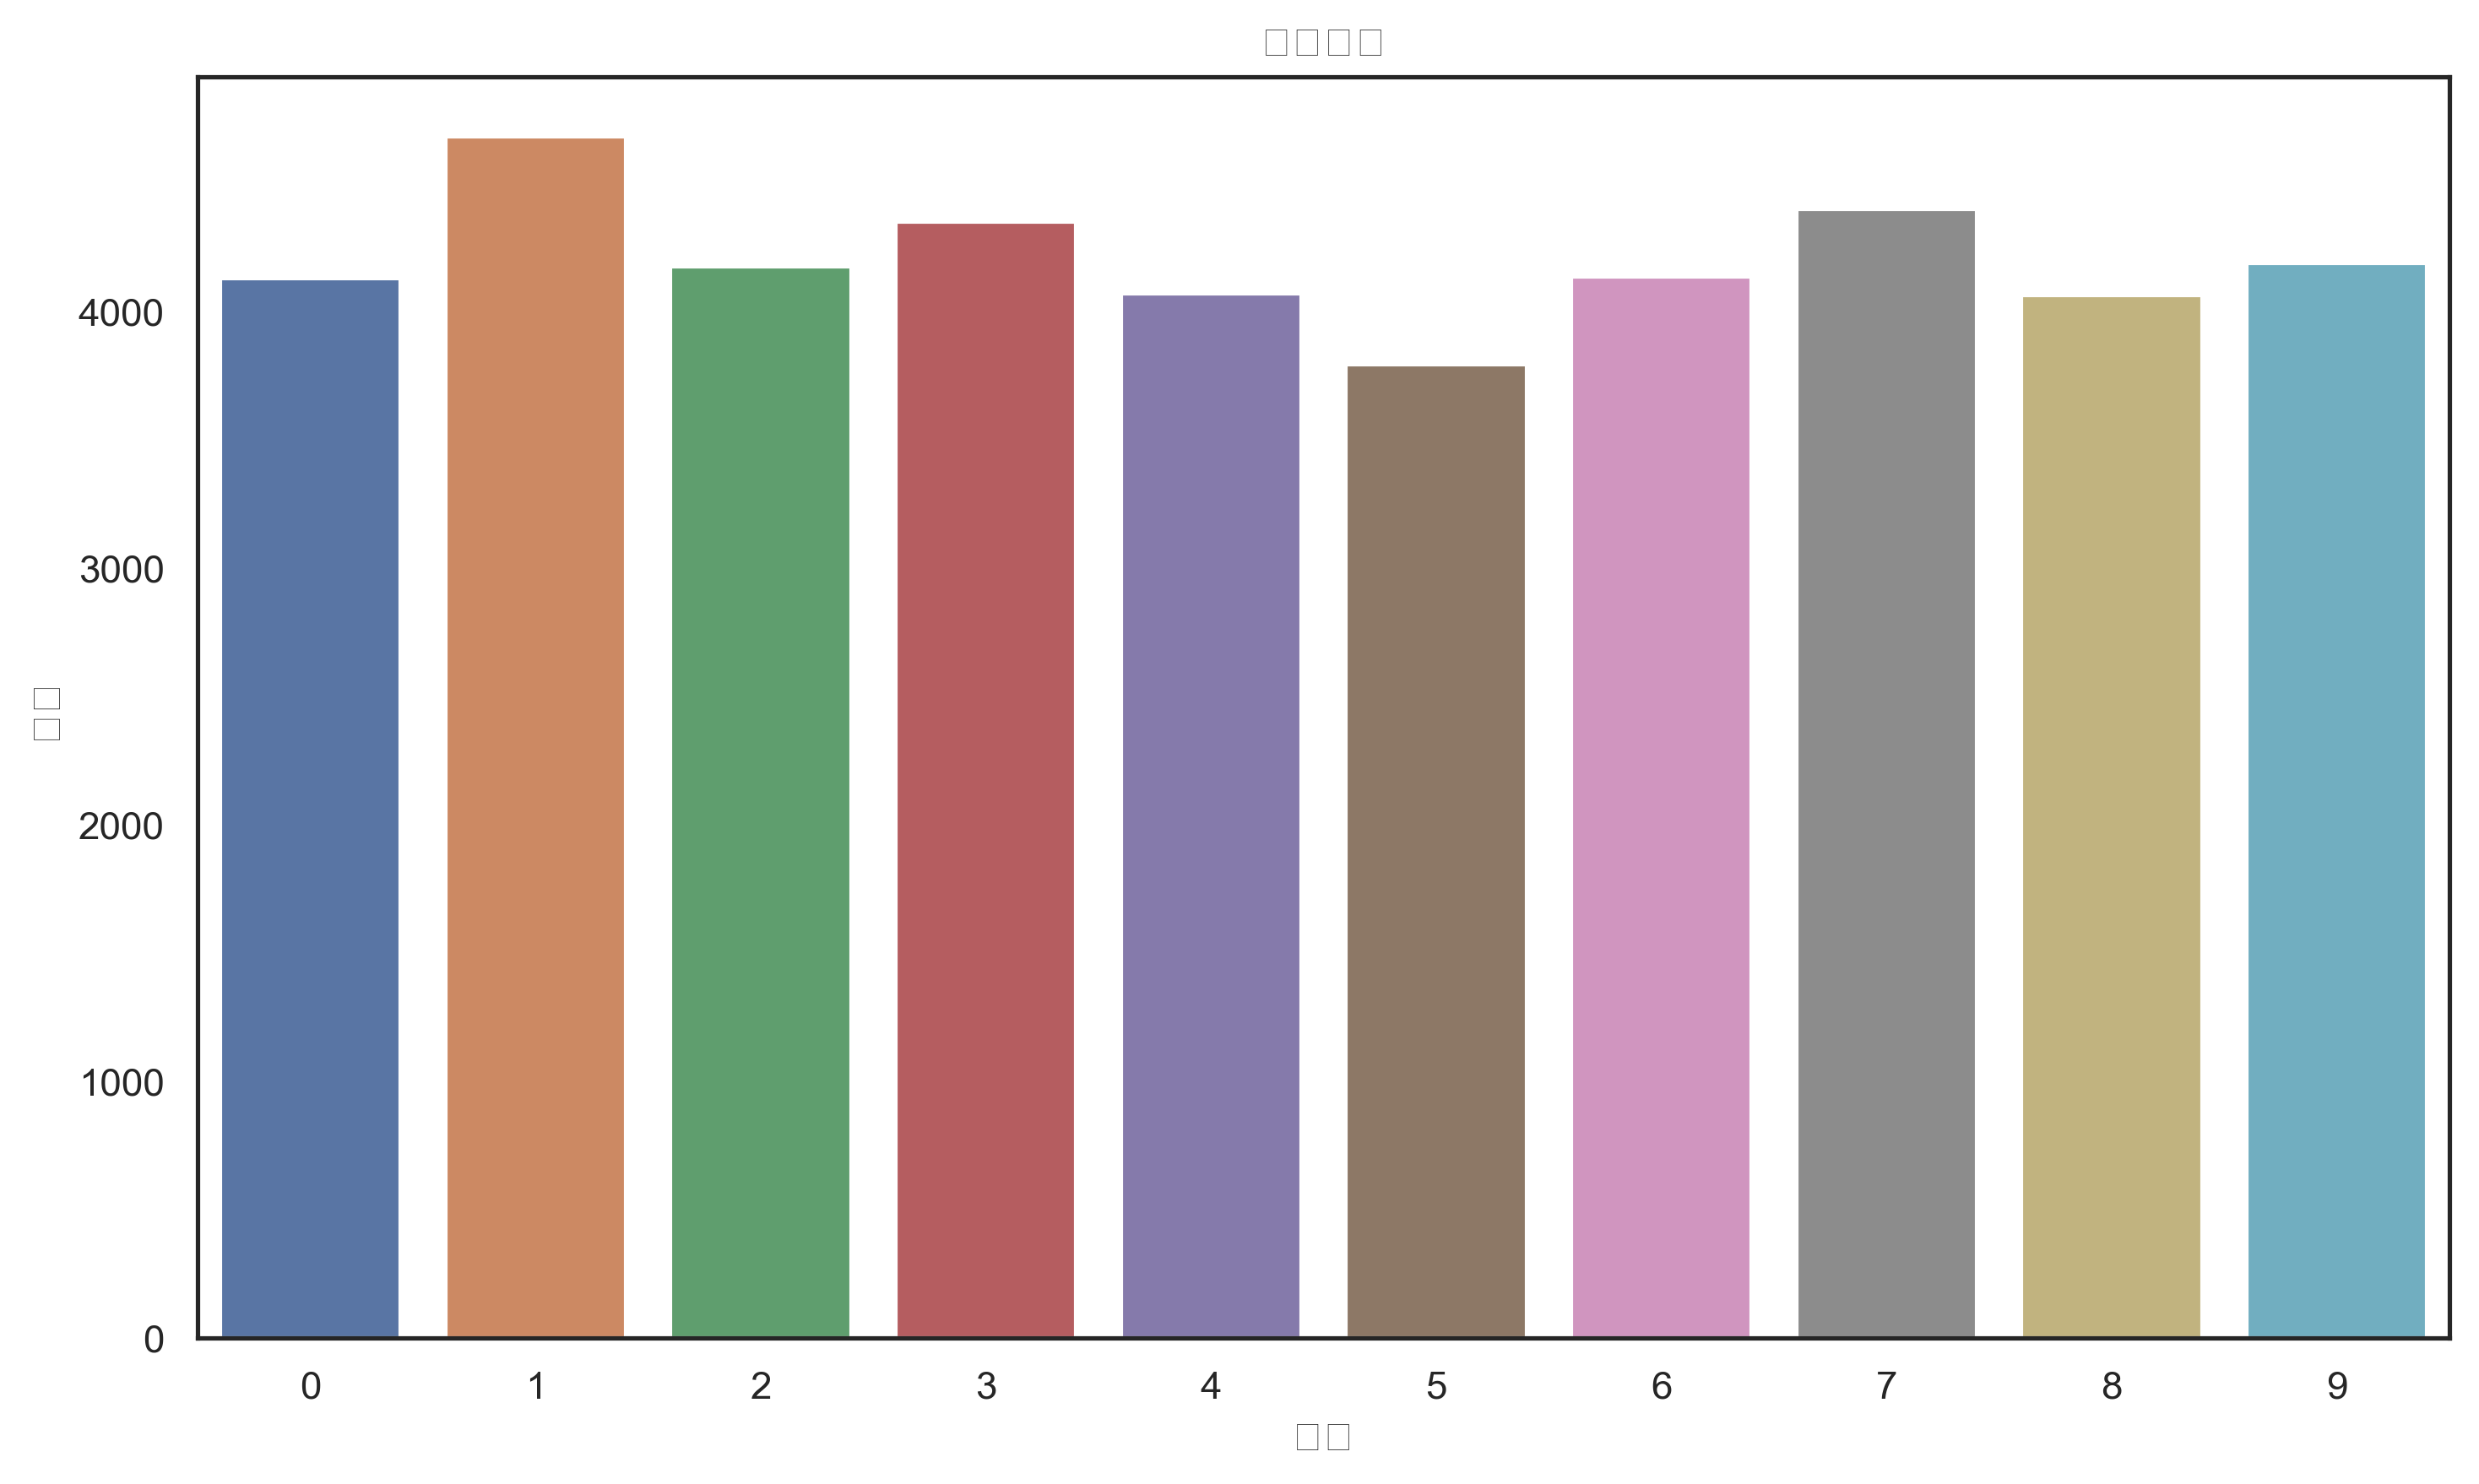
\includegraphics[width=\textwidth]{figures/digit_distribution.png}
                \caption{训练集中各数字的样本数量分布}
                \label{fig:digit_distribution}
            \end{subfigure}
            \hfill
            \begin{subfigure}[b]{0.48\textwidth}
                \centering
                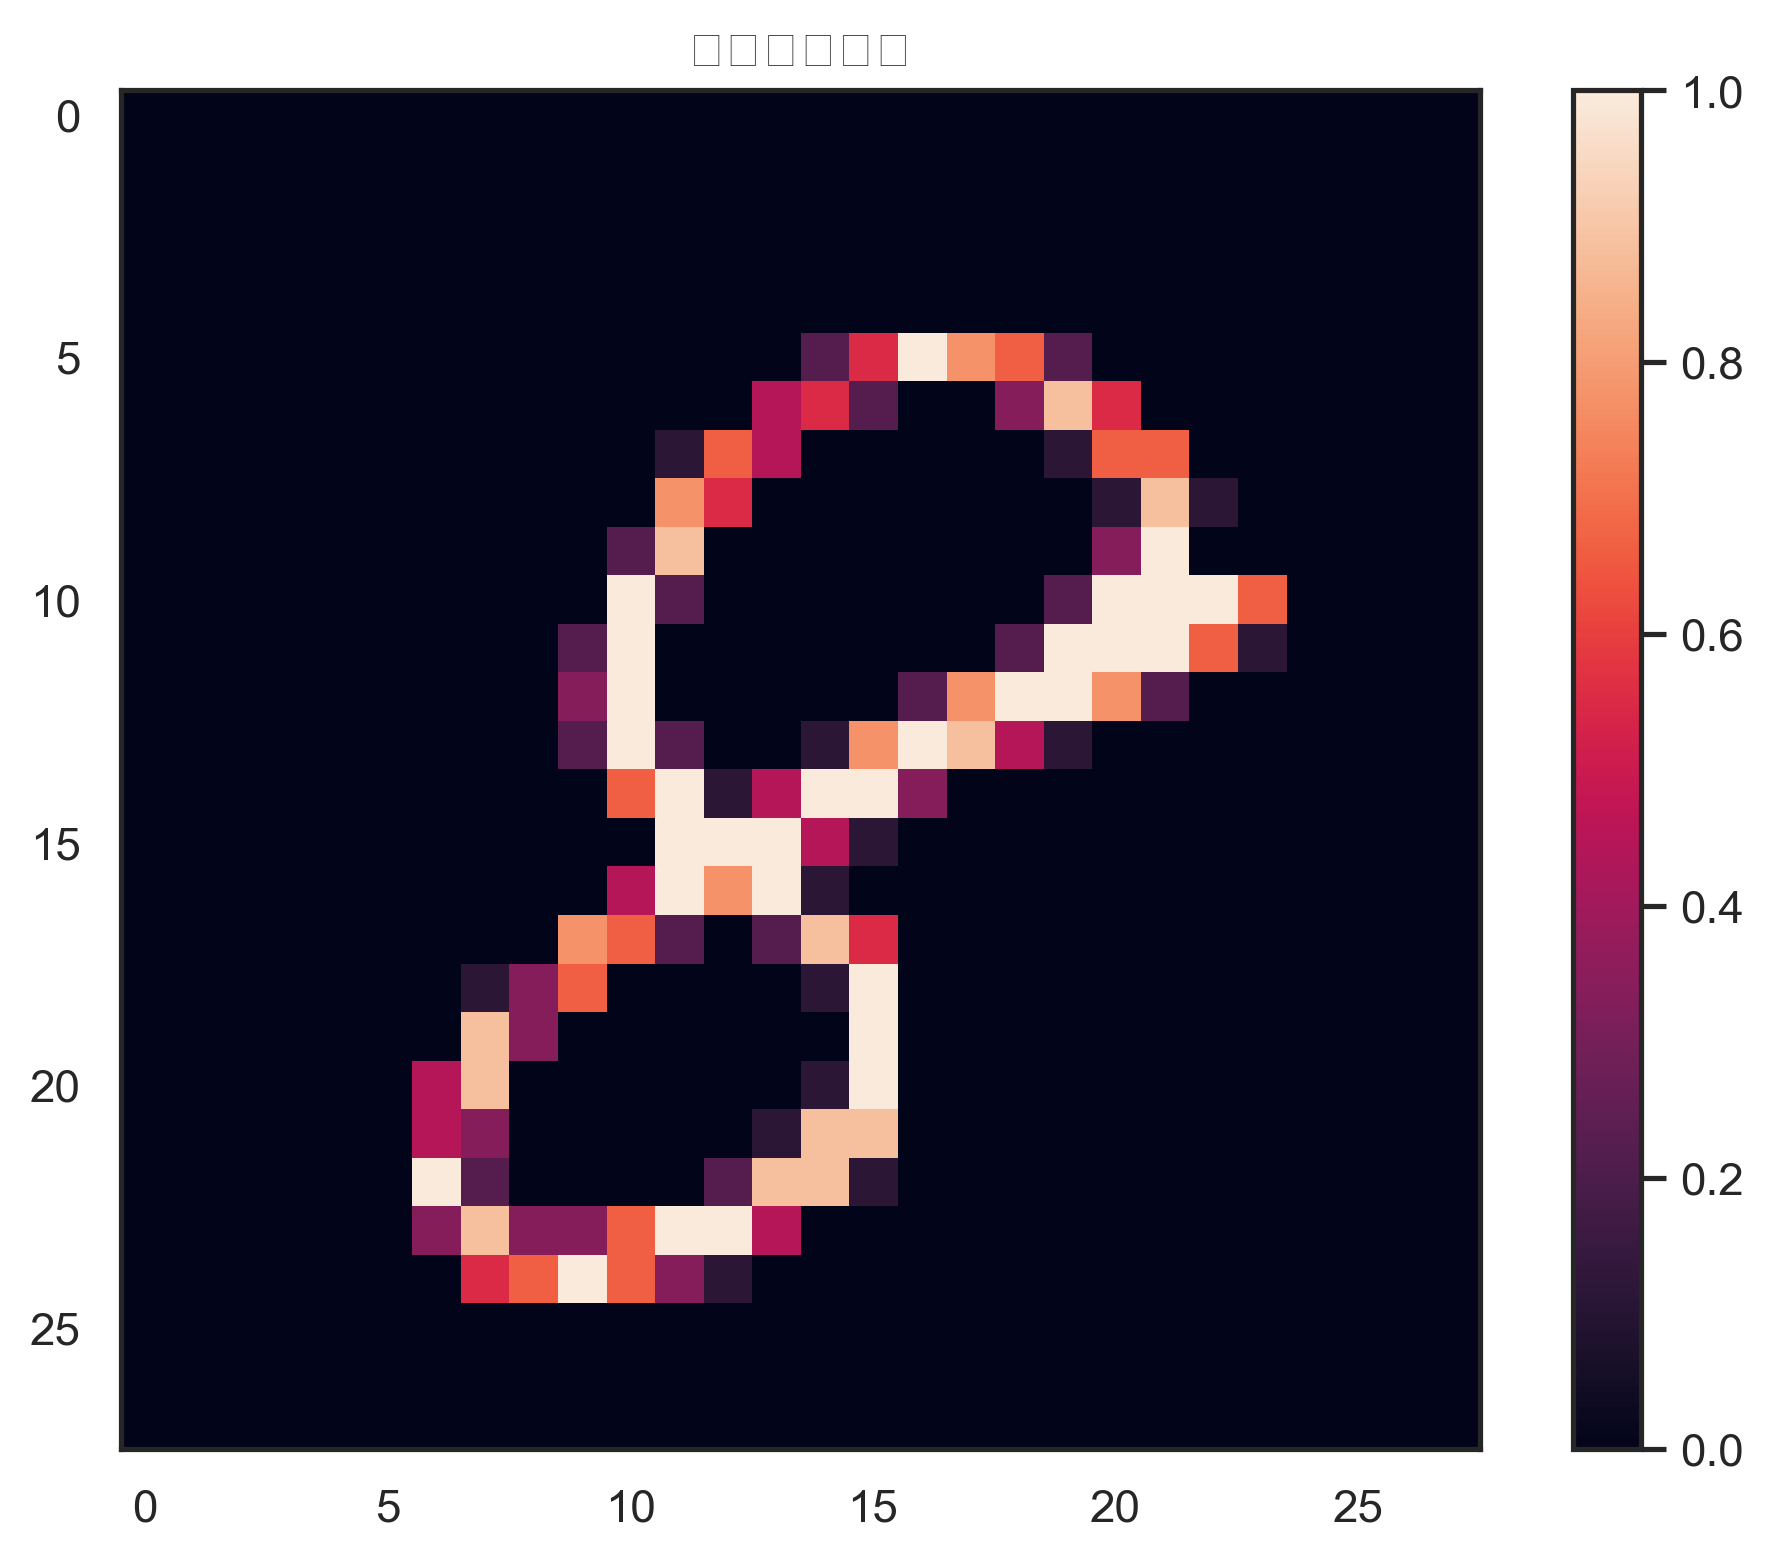
\includegraphics[width=0.8\textwidth]{figures/sample_digit.png}
                \caption{一个手写数字“8”的样本图像}
                \label{fig:sample_digit}
            \end{subfigure}
            \caption{手写数字数据集的数据探索可视化}
            \label{fig:digit_exploration}
        \end{figure}

        \paragraph{2. 模型评估与错误分析}
        模型训练完成后,我们需要对其性能进行深入评估。混淆矩阵(如图 \ref{fig:classification_evaluation}a)是一种强大的工具,它不仅展示了总体准确率,还清晰地揭示了模型容易将哪些类别混淆。例如,图中显示数字“4”有时会被错误地预测为“9”。进一步地,我们可以将这些被错误分类的样本单独提取出来进行可视化分析(如图 \ref{fig:classification_evaluation}b),这对于理解模型的弱点、进行针对性的优化至关重要。这些定性和定量的分析方法,与前述的精确率、召回率等公式共同构成了分类问题完整的评估体系。
        
        \begin{figure}[H]
            \centering
            \begin{subfigure}[b]{0.48\textwidth}
                \centering
                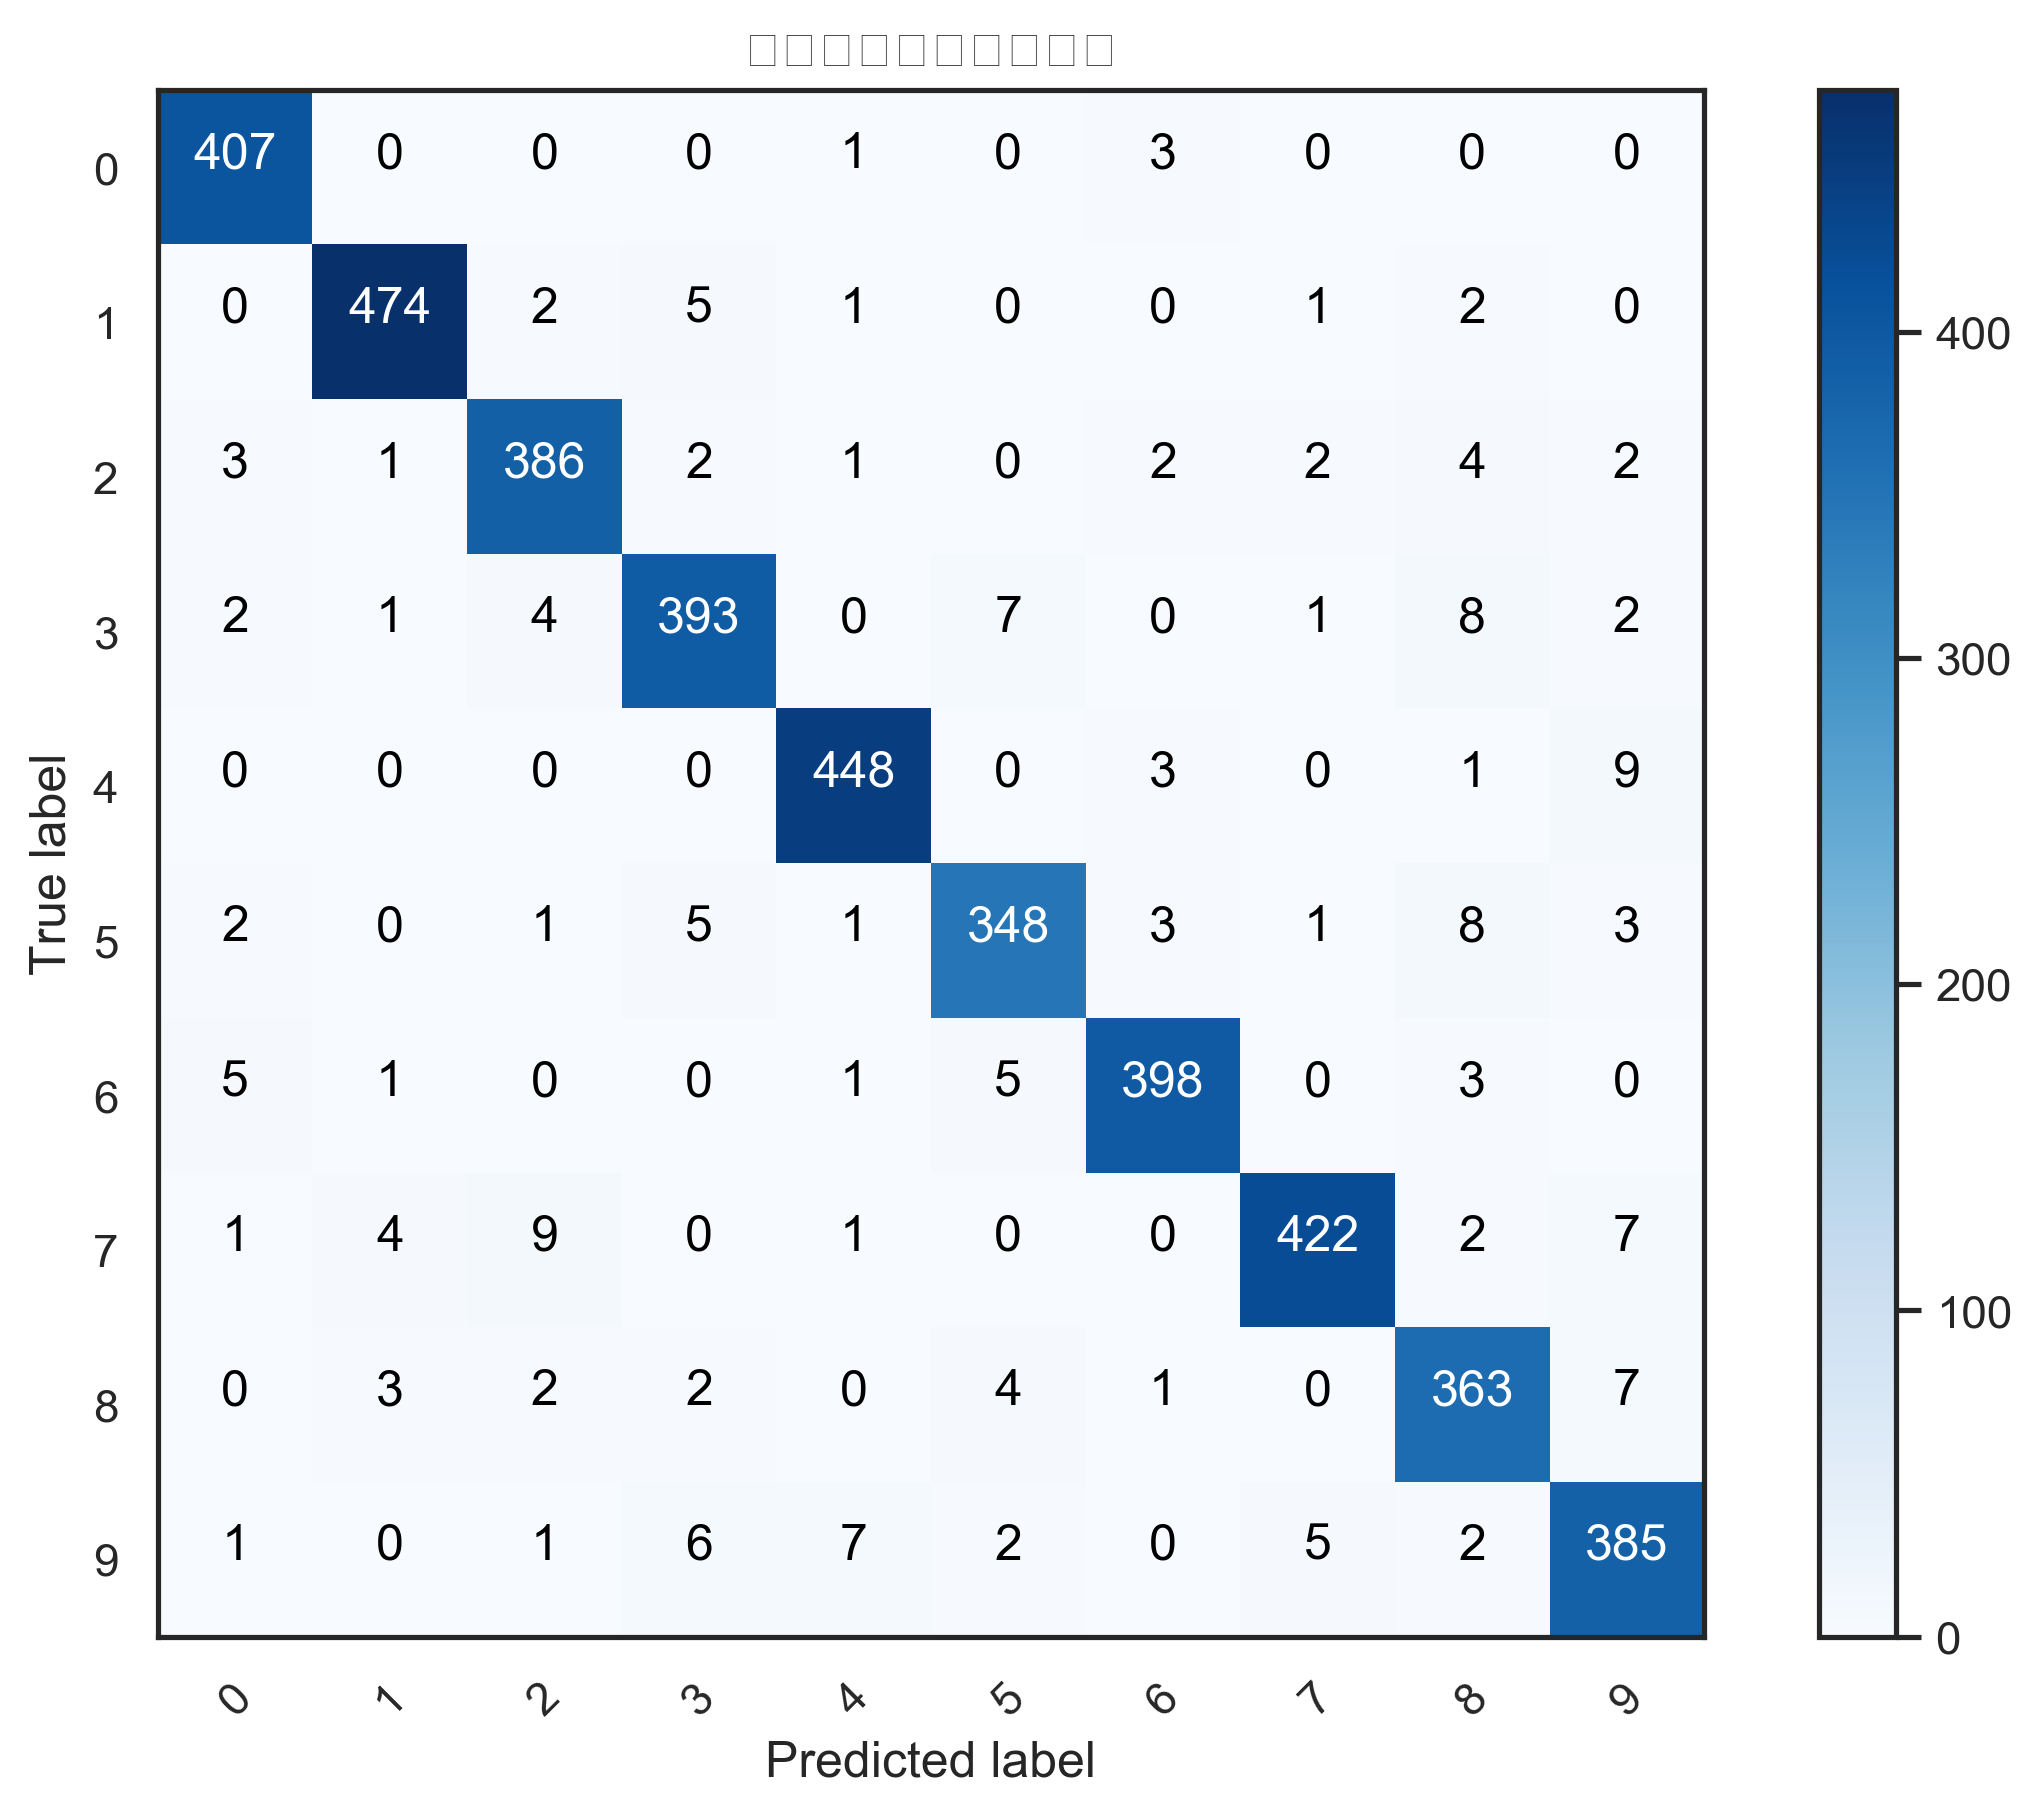
\includegraphics[width=\textwidth]{figures/confusion_matrix.png}
                \caption{模型在验证集上的混淆矩阵}
                \label{fig:confusion_matrix}
            \end{subfigure}
            \hfill
            \begin{subfigure}[b]{0.48\textwidth}
                \centering
                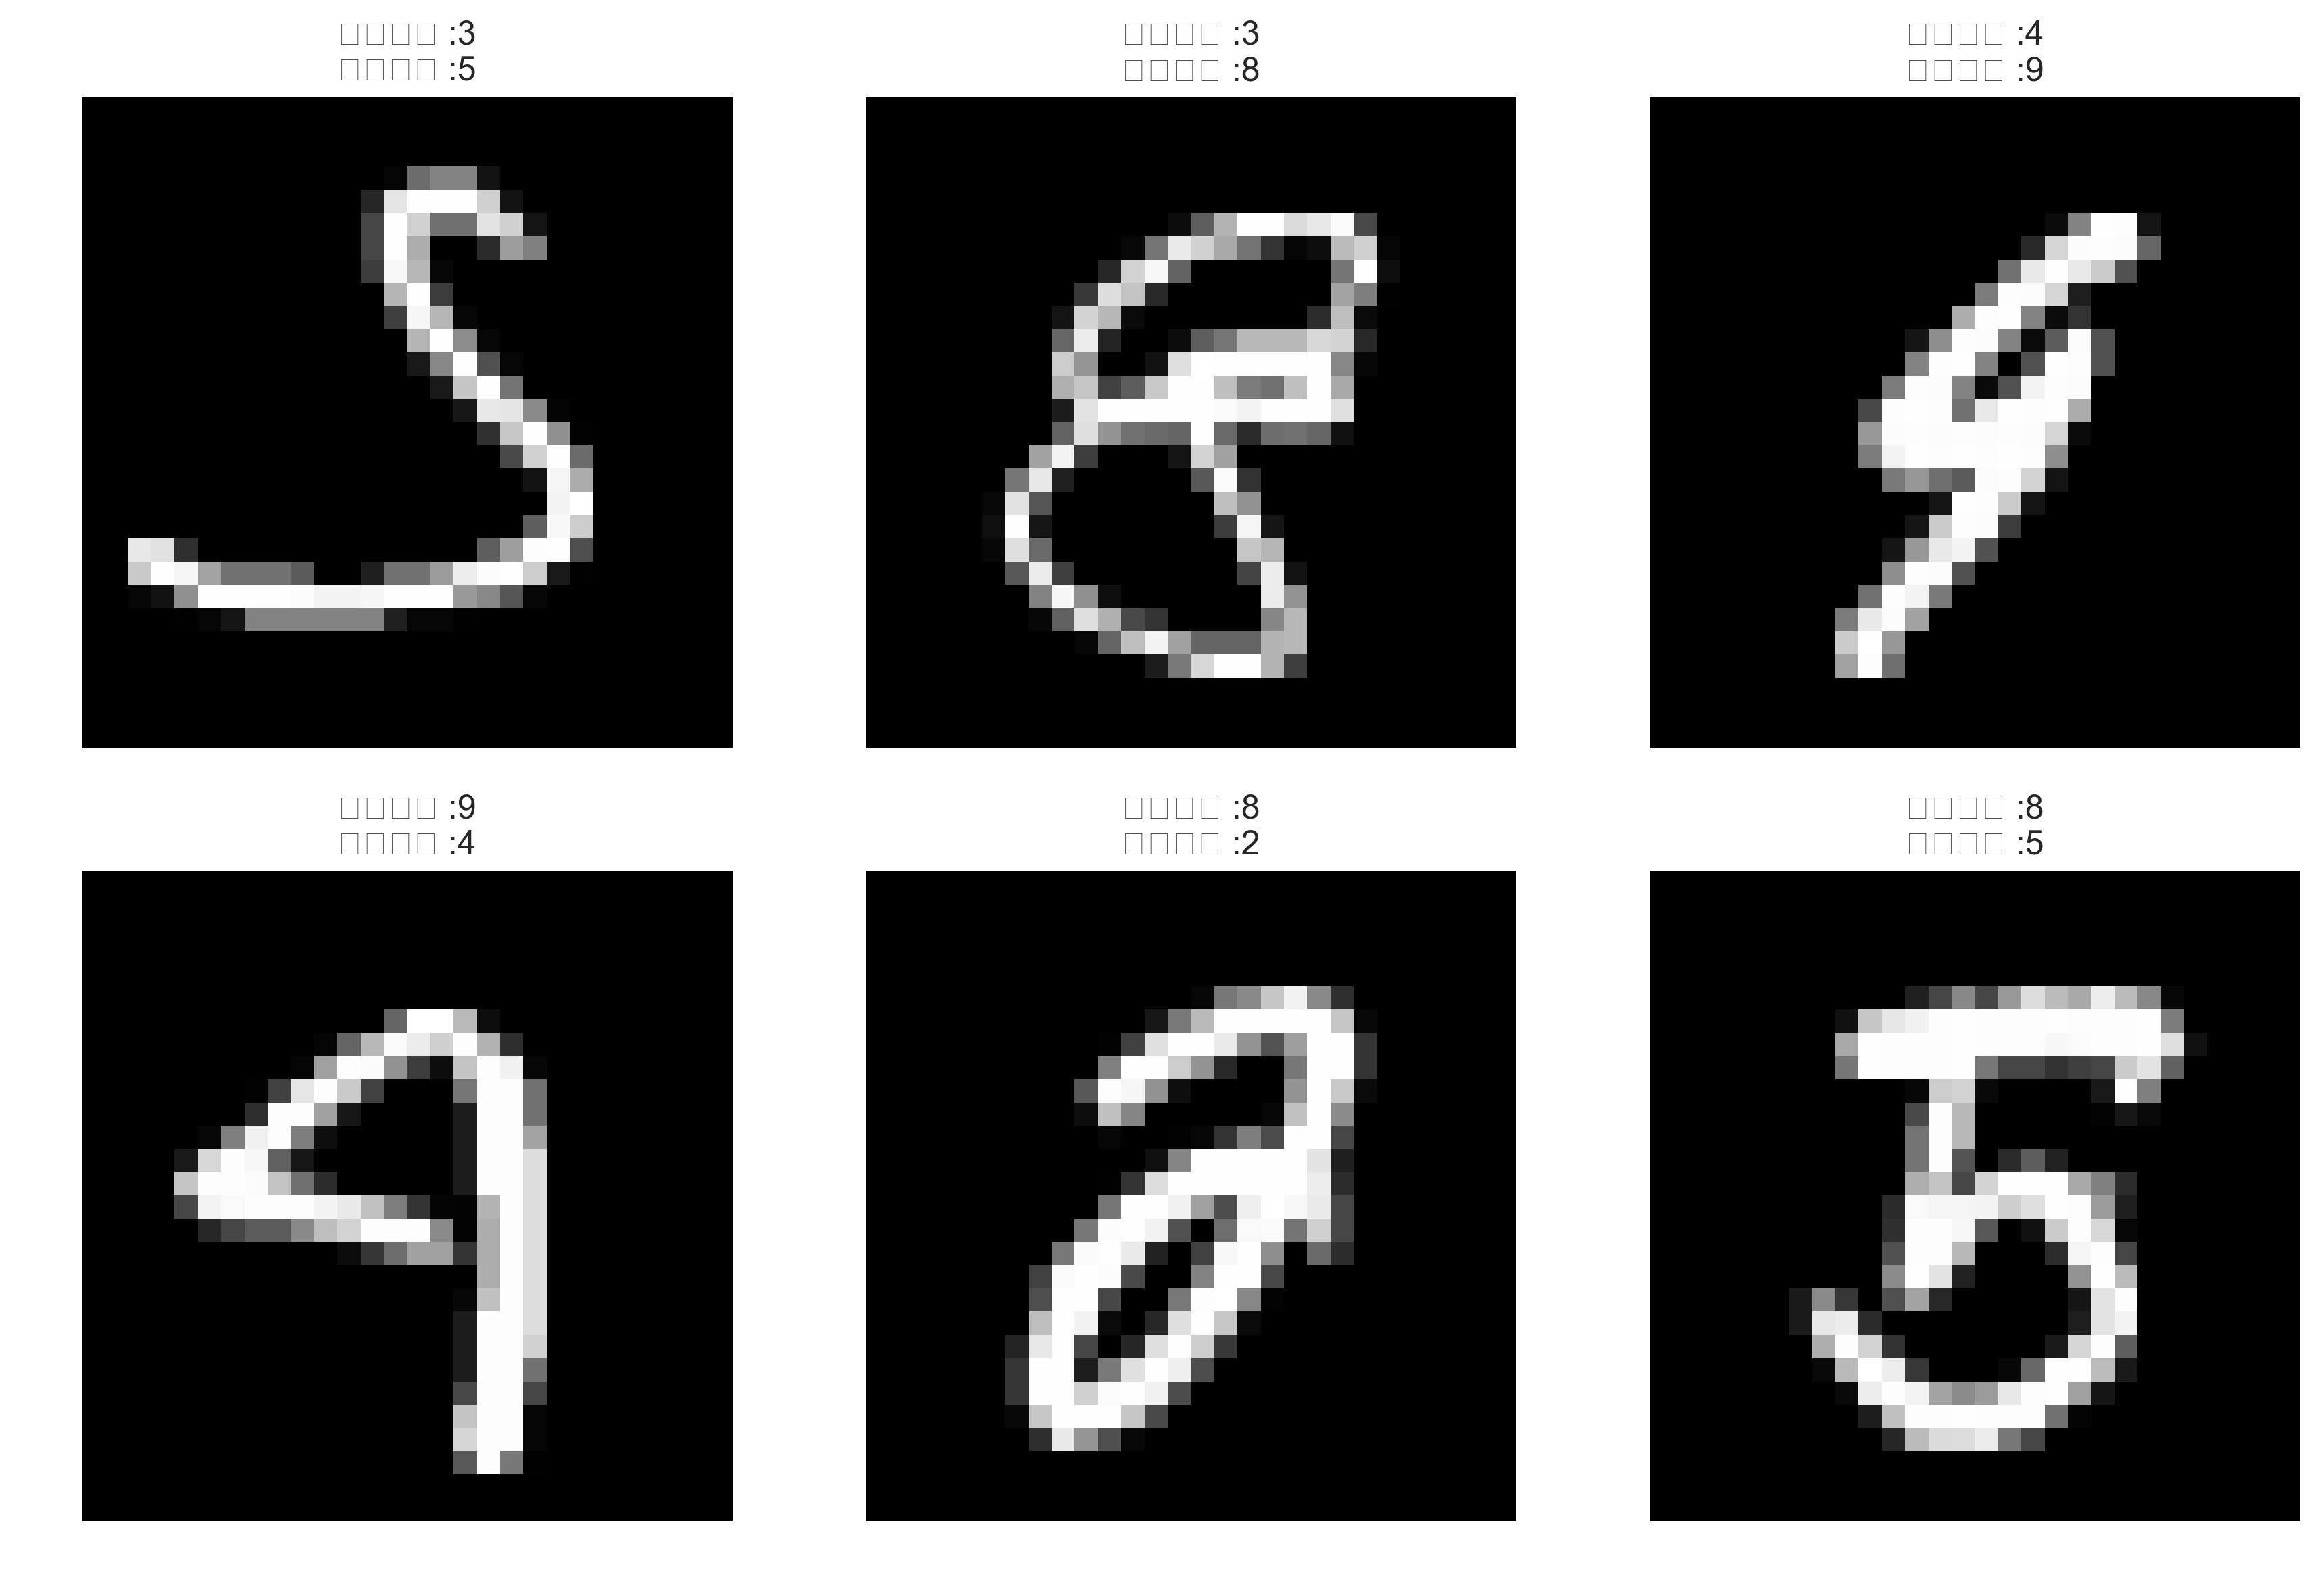
\includegraphics[width=\textwidth]{figures/error_analysis.png}
                \caption{模型错误分类的样本示例}
                \label{fig:error_analysis}
            \end{subfigure}
            \caption{分类模型的性能评估与错误分析}
            \label{fig:classification_evaluation}
        \end{figure}

    \item \textbf{回归(Regression):} 与分类不同,回归任务的目标是预测一个连续的数值。例如,根据房屋的面积、位置和房龄等特征来预测其售价。线性回归是最基础的回归模型,它试图找到一条直线(或超平面)来最佳地拟合数据点。在回归任务中,常用的损失函数是均方误差(Mean Squared Error, MSE),其定义为:
    $$ L_{MSE} = \frac{1}{N} \sum_{i=1}^{N} (y_i - \hat{y}_i)^2 $$
    其中 $y_i$ 是真实值,$\hat{y}_i$ 是模型的预测值。模型的目标是调整参数以最小化该损失函数。

    \subsubsection*{案例研究:线性回归的数学原理与实现}
    \label{sssec:lr_case_study}
    为了更具体地说明回归过程,我们以一个简单的线性回归为例,展示其从数据探索到模型建立的关键步骤和数学原理。
    
    \paragraph{1. 矩阵化模型与正规方程}
    在实践中,我们将多个样本的线性回归方程整合成矩阵形式。假设有 $N$ 个样本,每个样本有 $p$ 个特征,则模型可以表示为 $\underline{\boldsymbol{y}} = \boldsymbol{X} \underline{\boldsymbol{\theta}}$。最小化均方误差损失函数的过程,可以通过求解其对参数 $\boldsymbol{\theta}$ 的偏导数并令其为零来实现。这导出了一个可以直接计算出最优参数估计值 $\boldsymbol{\hat{\theta}}$ 的闭式解,称为\textbf{正规方程(Normal Equation)}:
    $$
    \boldsymbol{\hat{\theta}} = (\boldsymbol{X}^T\boldsymbol{X})^{-1}\boldsymbol{X}^T\boldsymbol{y}
    $$
    这个方程是许多线性回归库求解的基础。
    
    \paragraph{2. 实例数据分析与可视化}
    在一个具体的回归任务中,我们首先通过可视化来探索数据。图 \ref{fig:lr_data_exploration} 展示了数据探索的两个关键步骤:(a) 使用相关性热力图检查特征与目标值之间的线性关系强度;(b) 通过散点图直观地观察数据的分布趋势。
    
    \begin{figure}[H]
        \centering
        \begin{subfigure}[b]{0.48\textwidth}
            \centering
            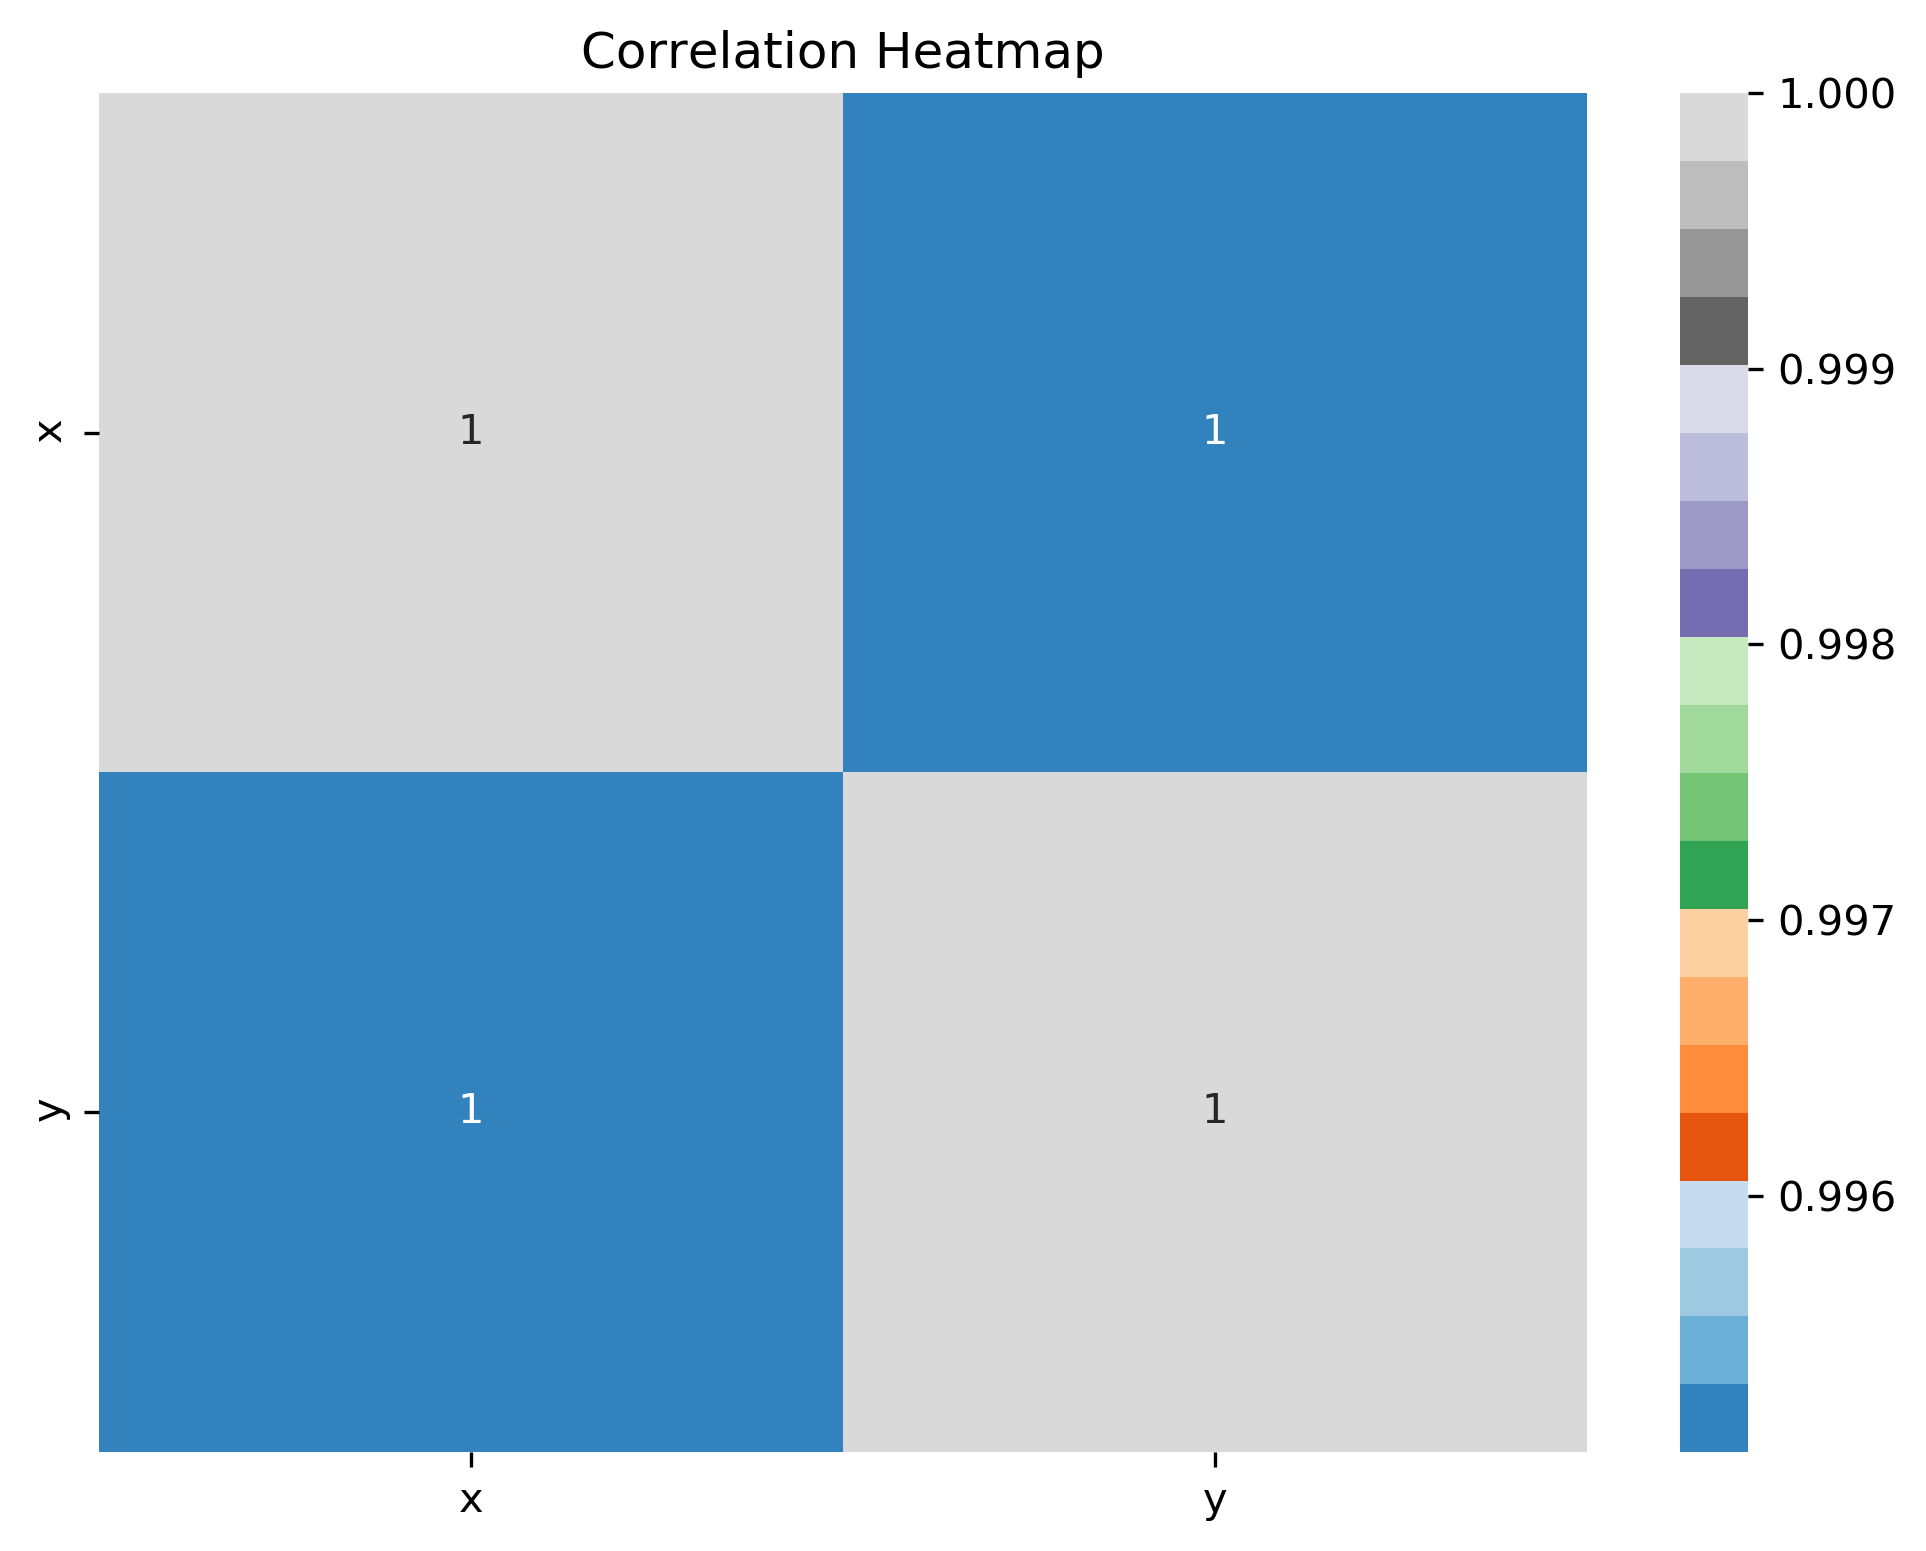
\includegraphics[width=\textwidth]{figures/correlation_heatmap.png}
            \caption{特征与目标值的相关性热力图}
            \label{fig:heatmap}
        \end{subfigure}
        \hfill
        \begin{subfigure}[b]{0.48\textwidth}
            \centering
            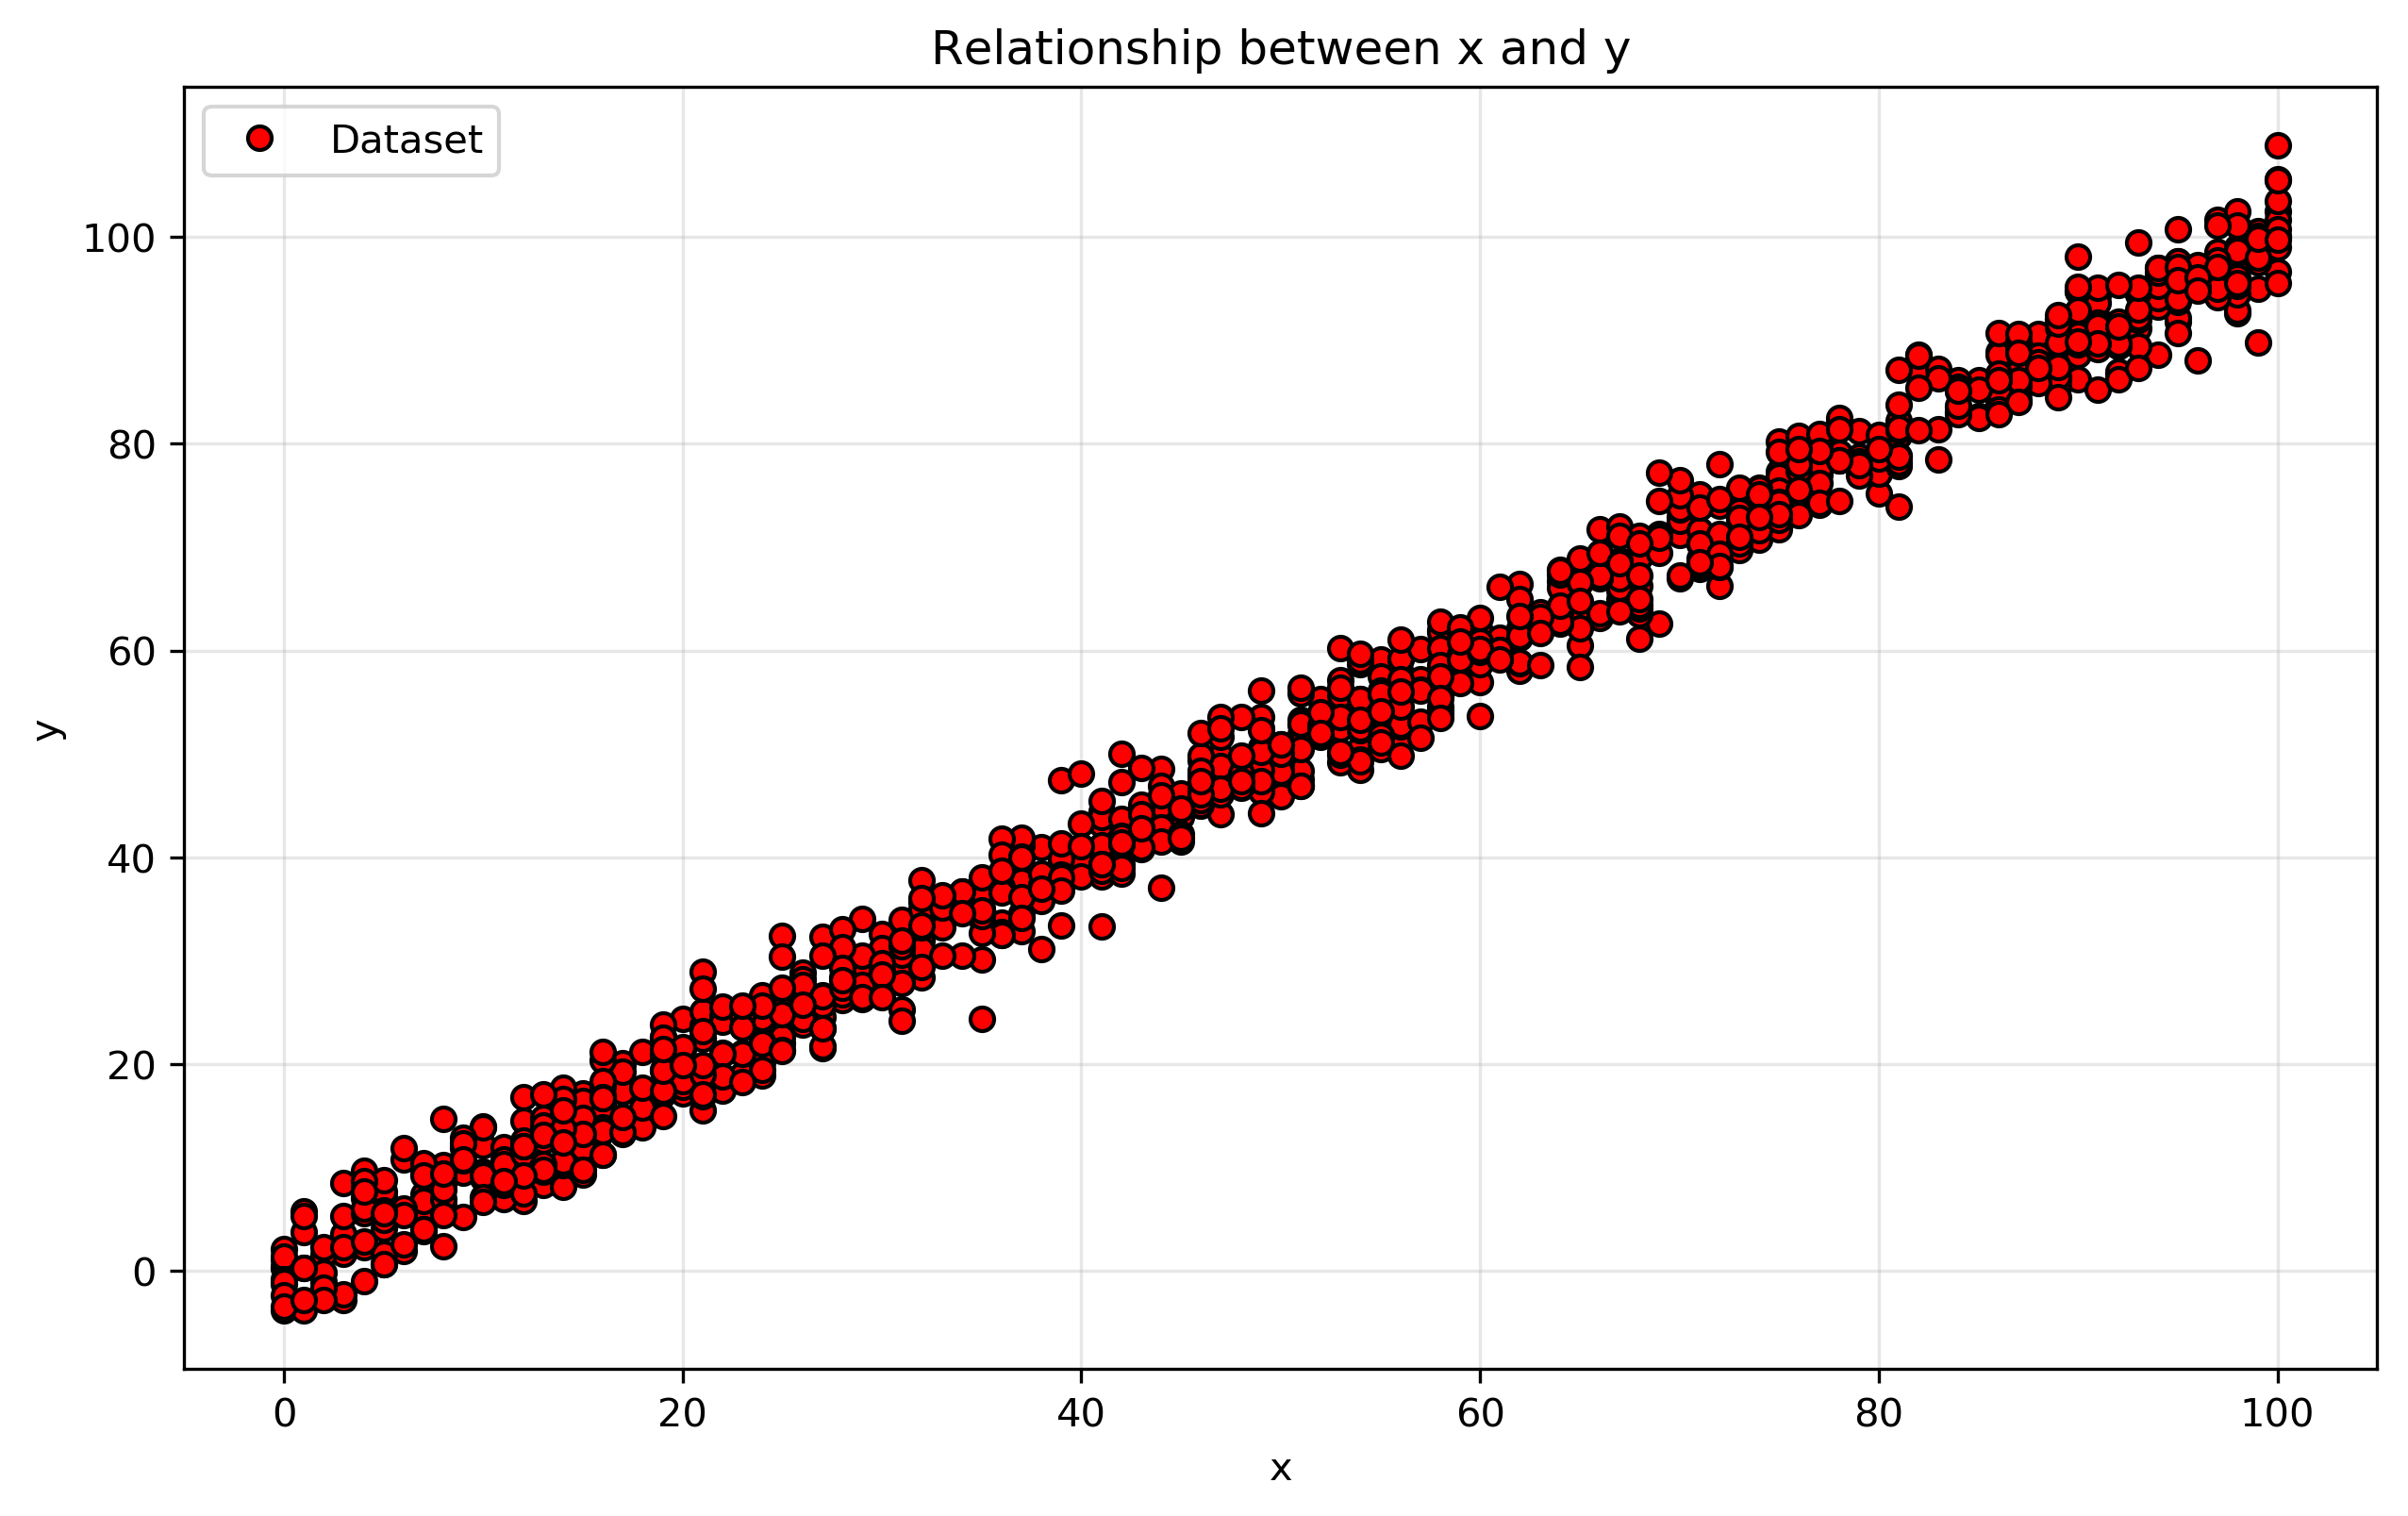
\includegraphics[width=\textwidth]{figures/data_scatter_plot.png}
            \caption{原始数据分布散点图}
            \label{fig:scatterplot}
        \end{subfigure}
        \caption{线性回归案例的数据探索可视化}
        \label{fig:lr_data_exploration}
    \end{figure}
    
    在确认数据适合进行线性回归后,我们应用上述正规方程求解模型参数,并对模型进行评估。图 \ref{fig:lr_fit_results} 展示了线性回归模型的概念与最终拟合效果:(a) 概念图清晰地展示了线性回归的目标是找到一条最佳拟合直线来描述数据点的趋势;(b) 将训练好的模型应用于测试集,并将预测结果(蓝色直线)与真实的测试数据点(红色点)进行对比,以评估模型的泛化能力。
    
    \begin{figure}[H]
        \centering
        \begin{subfigure}[b]{0.48\textwidth}
            \centering
            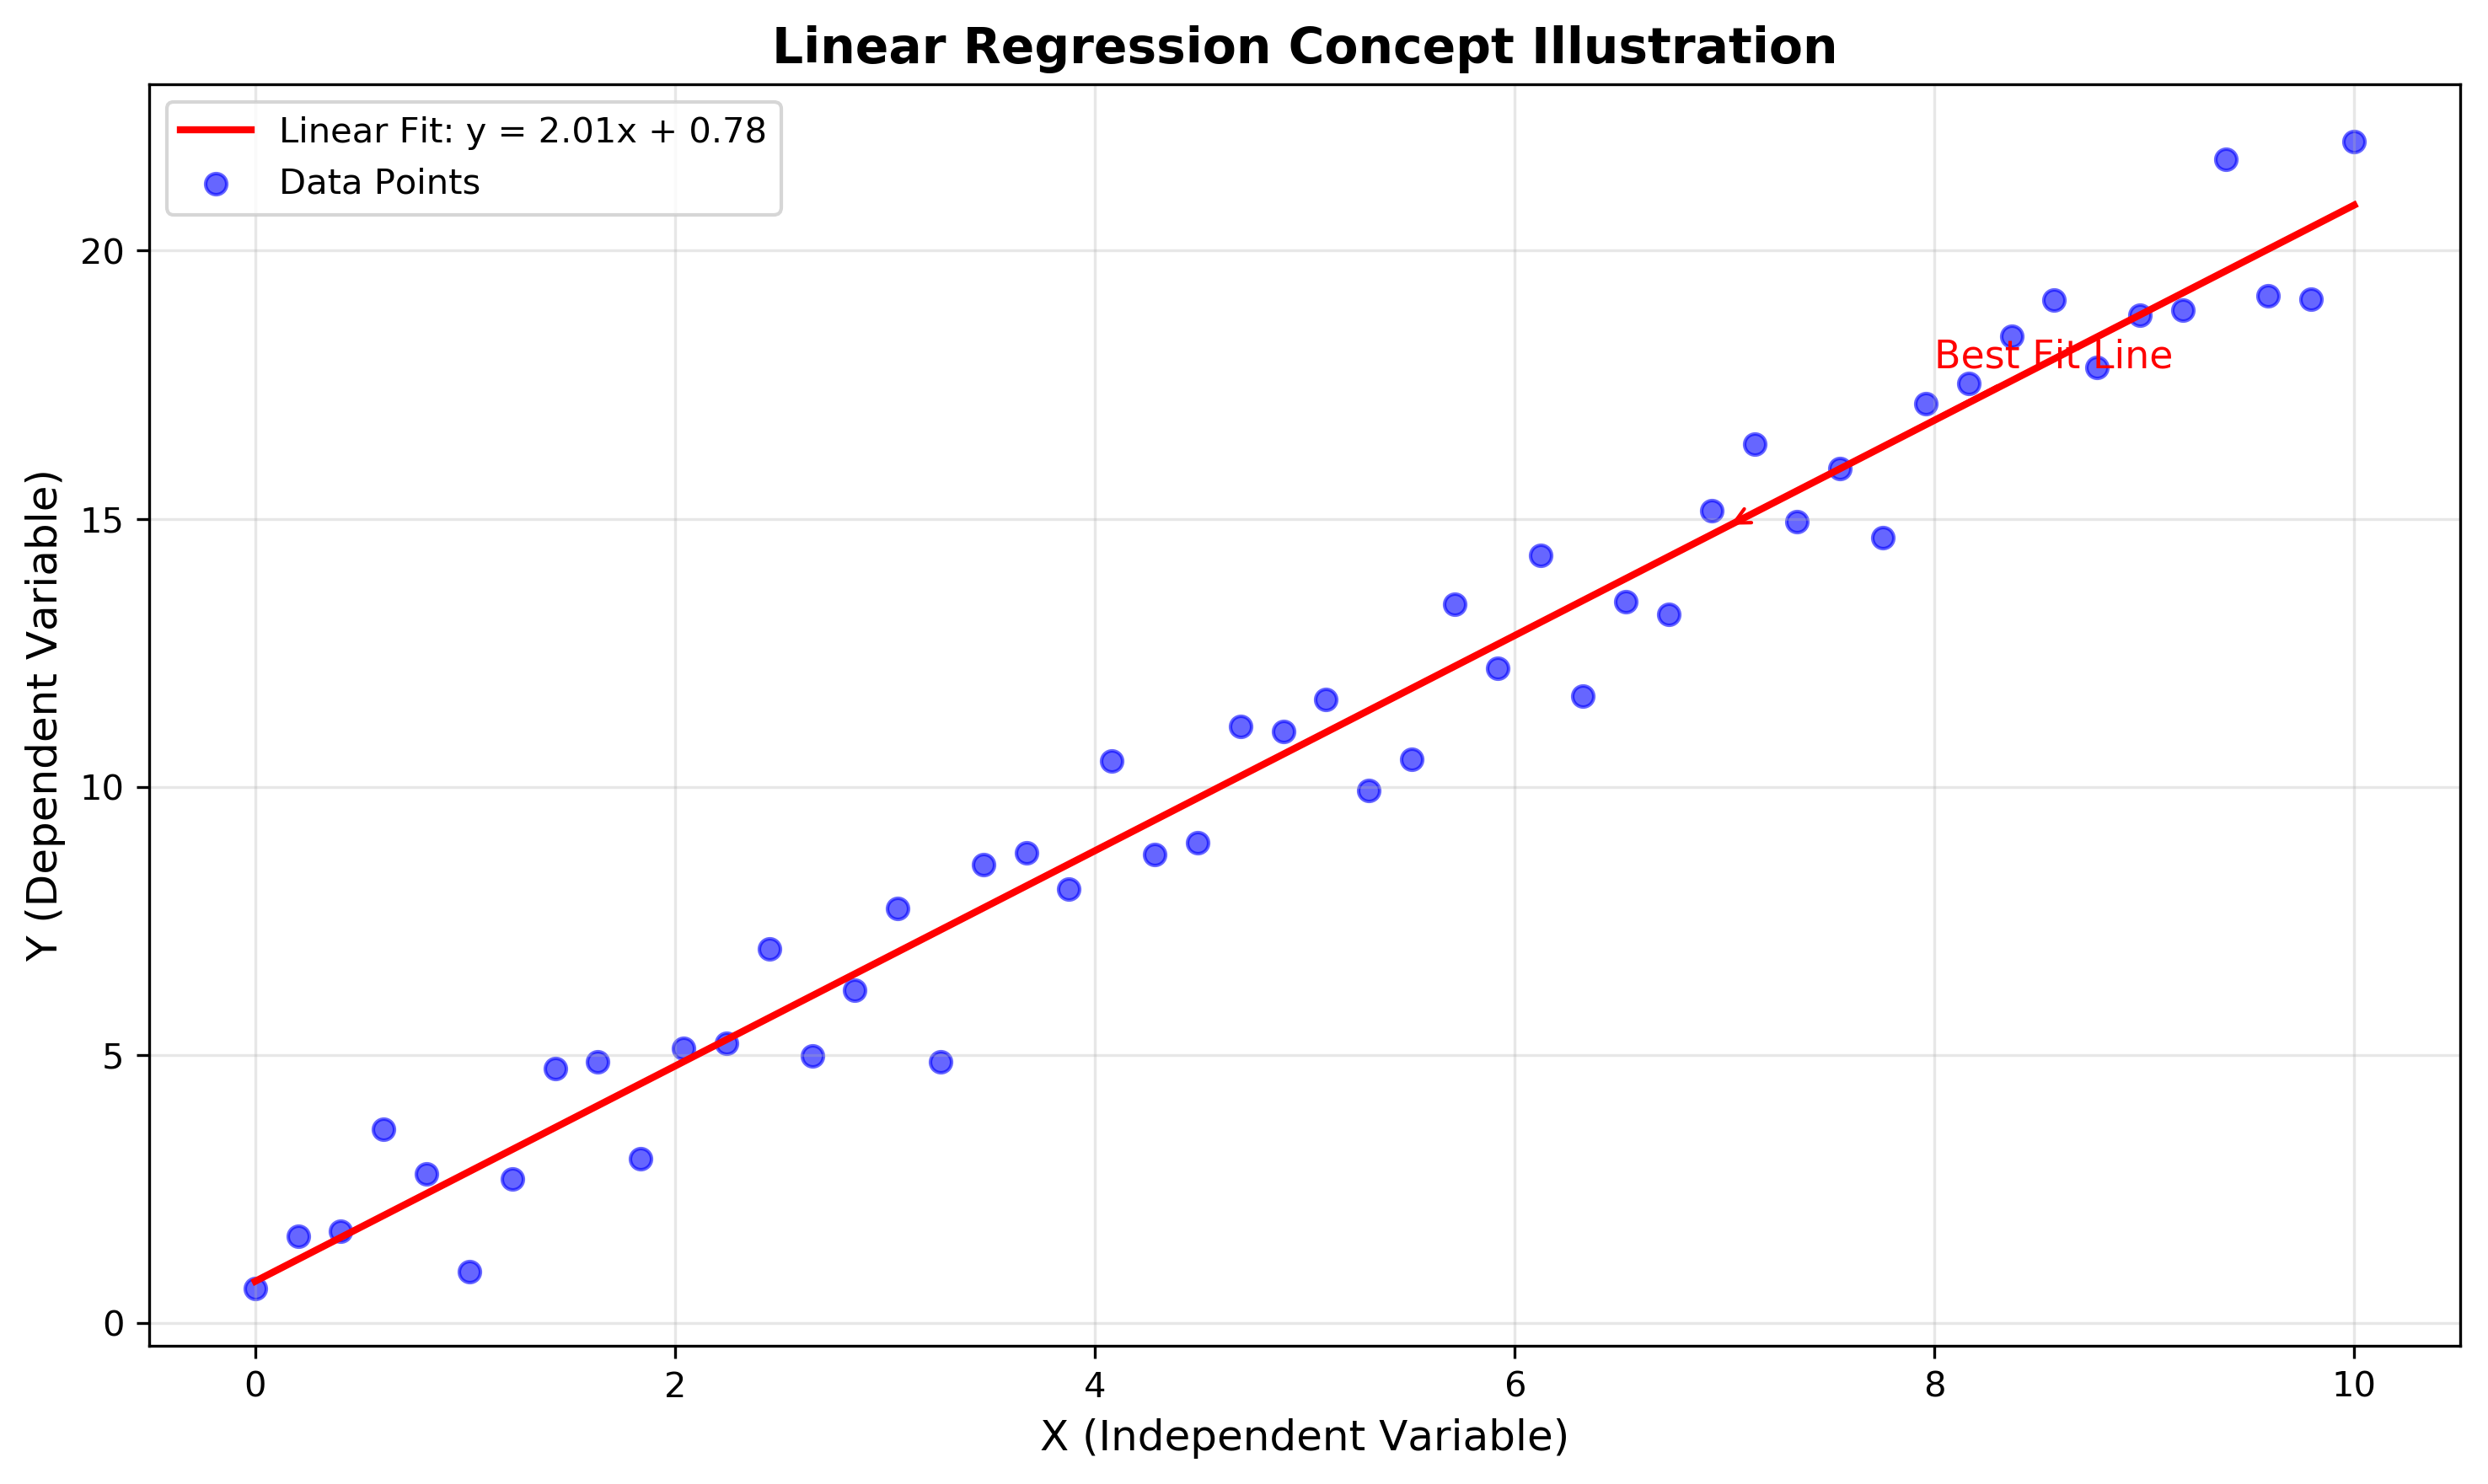
\includegraphics[width=\textwidth]{figures/linear_regression_concept.png}
            \caption{线性回归概念示意图}
            \label{fig:lr_concept}
        \end{subfigure}
        \hfill
        \begin{subfigure}[b]{0.48\textwidth}
            \centering
            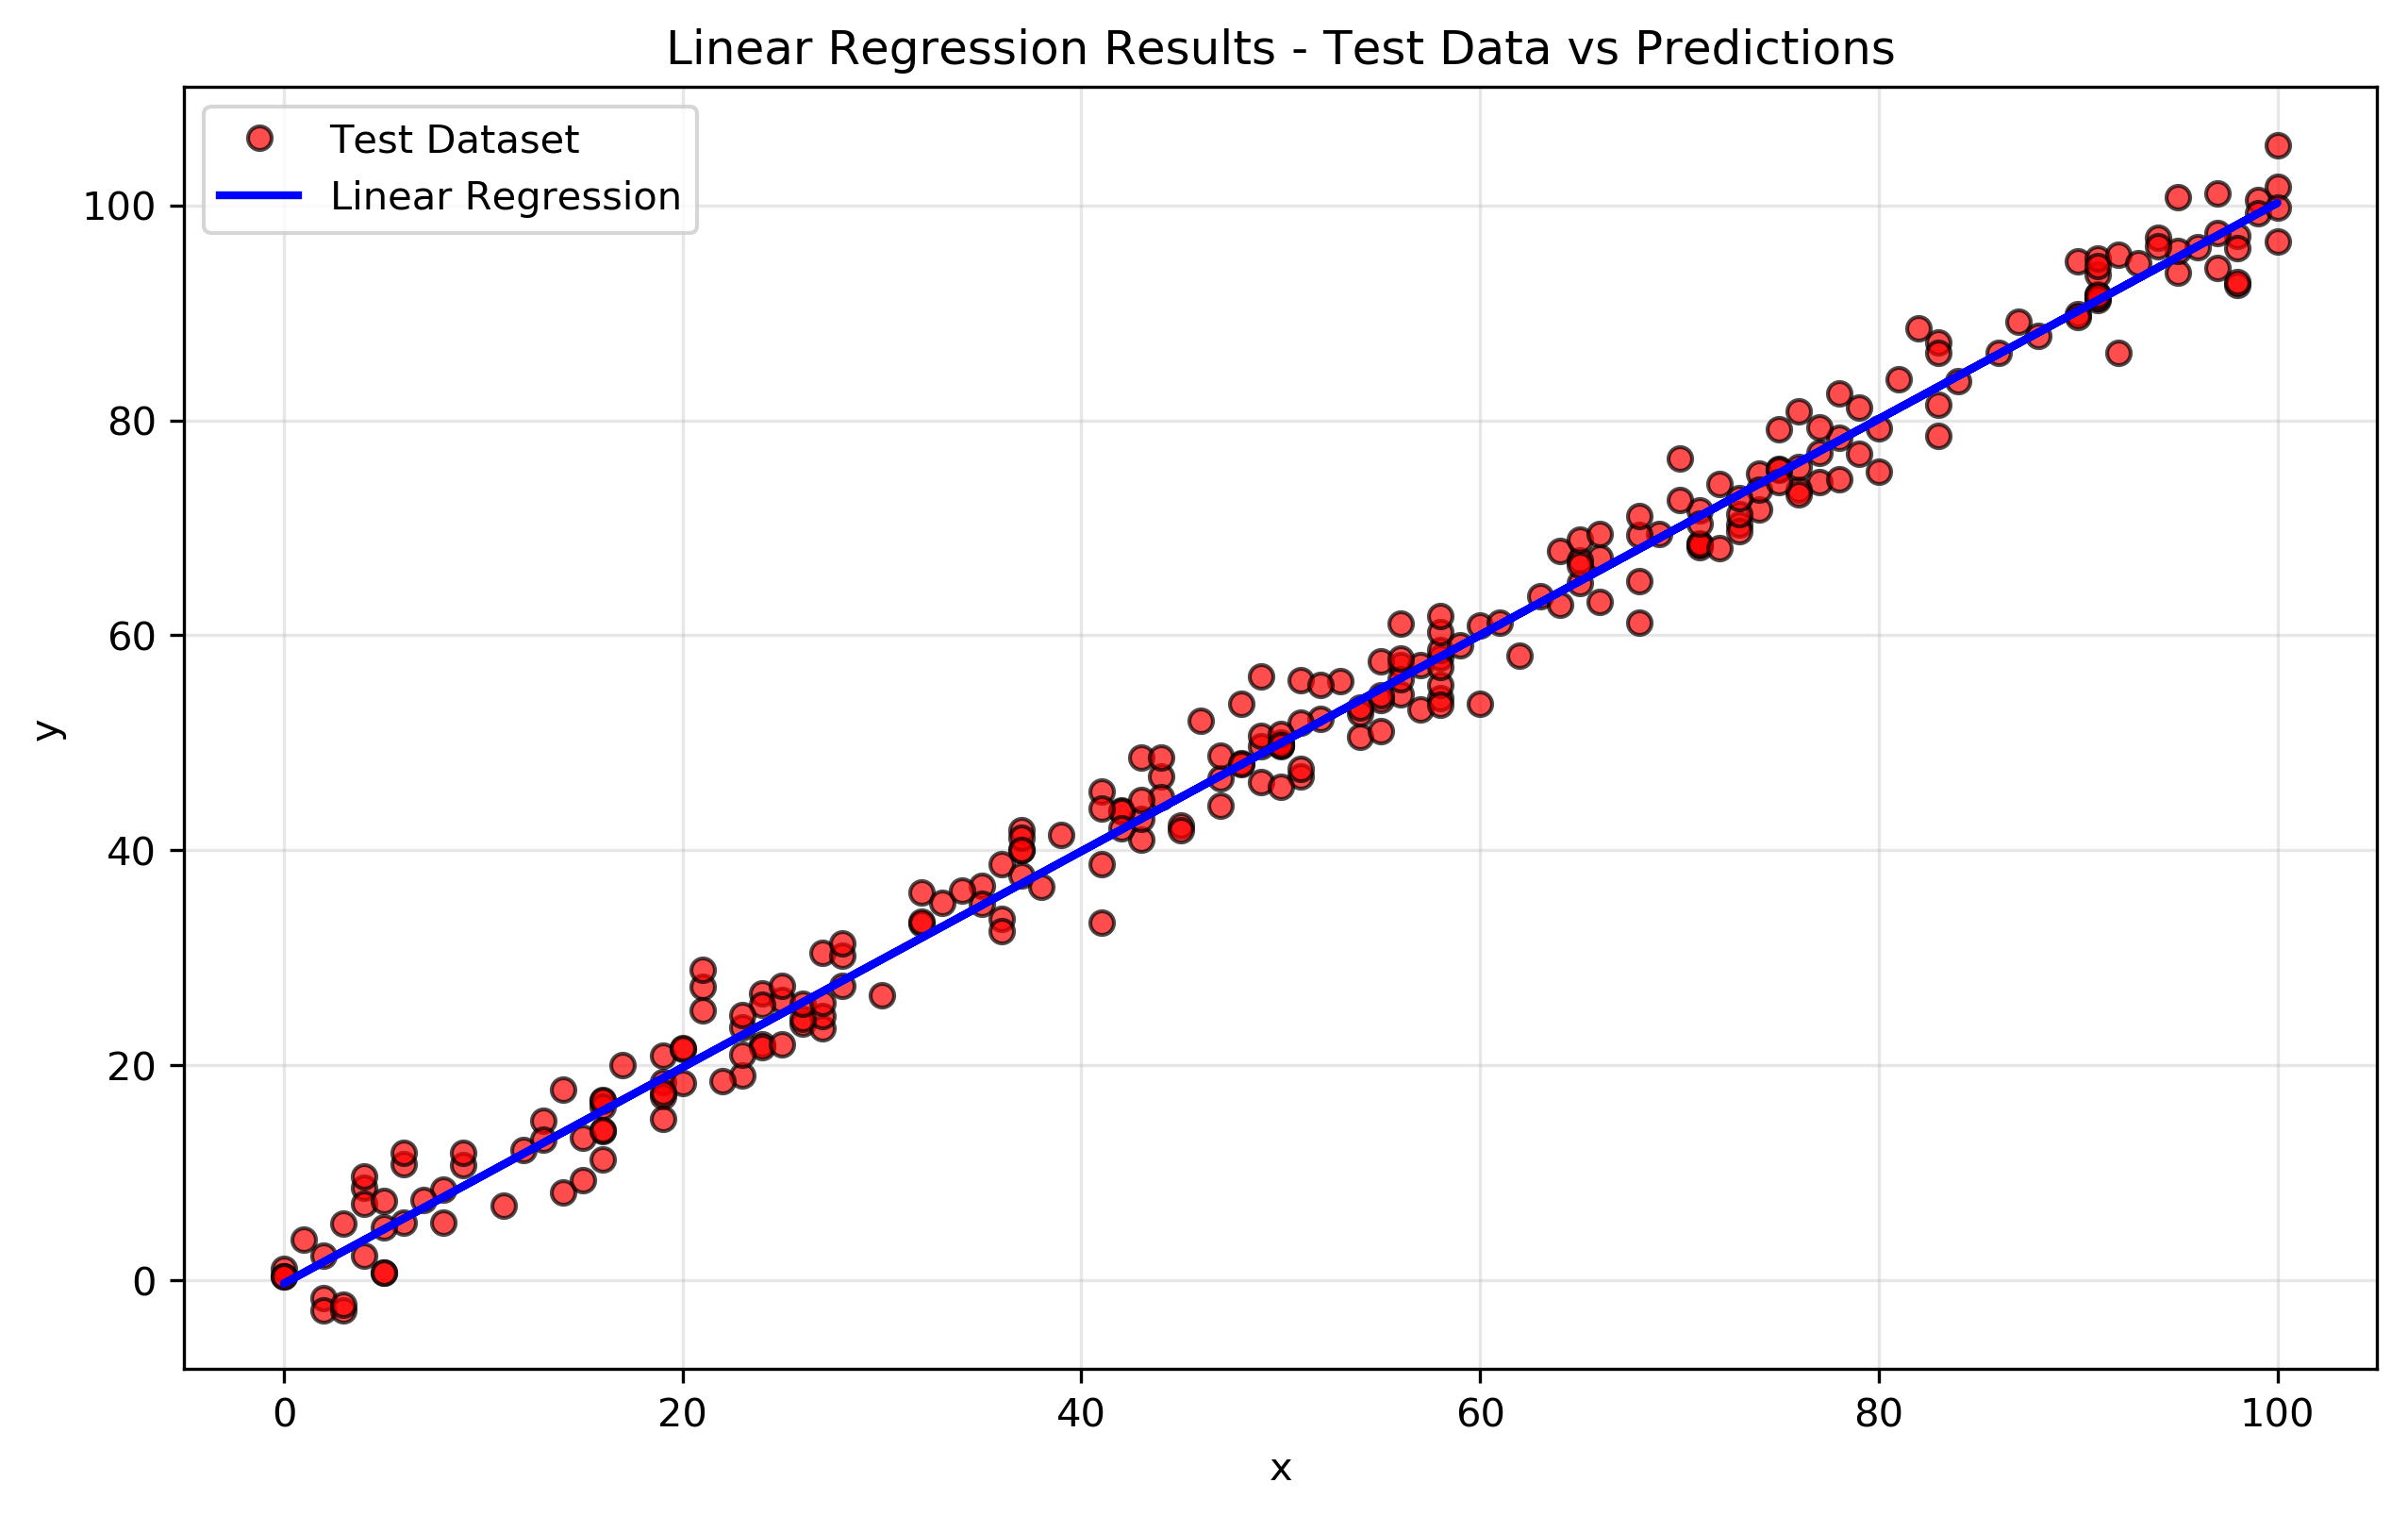
\includegraphics[width=\textwidth]{figures/linear_regression_results.png}
            \caption{模型在测试集上的拟合效果}
            \label{fig:lr_results}
        \end{subfigure}
        \caption{线性回归模型概念与拟合结果}
        \label{fig:lr_fit_results}
    \end{figure}

\end{itemize}

\subsection{无监督学习}
\label{ssec:unsupervised_learning}
无监督学习处理的是没有标签的数据,其目标是发现数据本身内在的结构、模式或关系 \cite{neuer2024unsupervised}。
\begin{itemize}
    \item \textbf{聚类(Clustering):} 聚类是将数据集中的样本划分为若干个相似的组(或簇),使得同一簇内的样本彼此相似,而不同簇的样本则相异。K-均值(K-Means)算法是聚类中最经典的算法之一,它通过迭代地将样本分配给最近的簇中心,并更新簇中心的位置,来最小化簇内样本的平方误差和。
    \item \textbf{降维(Dimensionality Reduction):} 降维旨在保留数据主要信息的前提下,减少数据的特征数量。这不仅可以降低计算复杂度和存储需求,还有助于可视化和去除噪声。主成分分析(Principal Component Analysis, PCA)是一种广泛应用的线性降维方法,它通过寻找数据方差最大的方向(即主成分)来构建一个新的、更低维的特征空间。
\end{itemize}

\subsection{强化学习}
\label{ssec:reinforcement_learning}
强化学习(RL)的灵感来源于行为心理学,它关注智能体(Agent)如何在一个环境中通过与环境的交互来学习最优的行动策略,以最大化其获得的累积奖励 \cite{shakya2023reinforcement}。
\begin{itemize}
    \item \textbf{核心原理:} 强化学习系统包含智能体、环境、状态、行动和奖励等核心要素。智能体根据当前状态选择一个行动,环境接收该行动后会转换到一个新的状态,并反馈给智能体一个奖励信号。智能体的目标就是学习一个策略(Policy),即从状态到行动的映射,来最大化其长期累积奖励。
    \item \textbf{经典算法:}
        \begin{itemize}
            \item \textbf{Q-learning:} Q-learning是一种经典的基于价值的强化学习算法。它通过学习一个动作价值函数(Q-function),$Q(s, a)$,来评估在状态$s$下采取行动$a$所能带来的未来回报。通过不断地与环境交互并使用贝尔曼方程(Bellman Equation)来迭代更新Q值,智能体最终能够学会在任何状态下选择Q值最大的行动。
            Q-learning 通过不断地与环境交互来迭代更新Q表格中的值。其核心的更新规则基于贝尔曼方程,具体如下:
			\[
				Q(s_{t},a_{t})\leftarrow Q(s_{t},a_{t})+\alpha[r_{t+1}+\gamma~max_{a}Q(s_{t+1},a)-Q(s_{t},a_{t})]
			\]
			其中:
			\begin{itemize}
				\item $s_t$ 和 $a_t$ 分别是当前时刻的状态和采取的行动。
				\item $\alpha$ 是学习率(Learning Rate),决定了新信息在多大程度上覆盖旧信息。
				\item $r_{t+1}$ 是在状态s₁采取行动后获得的即时奖励。
				\item $\gamma$ 是折扣因子(Discount Factor),衡量了未来奖励的重要性。
				\item $s_{t+1}$ 是下一个状态。
				\item $maxa Q(St+1, a)$是对下一个状态所有可能行动的Q值的最大预估,代表了对未来回报的最佳期望。
			\end{itemize}
			智能体的训练实验是否成功,就看Q函数最终能否收敛,从而指导智能体在每个状态下都能做出最优决策。
            \item \textbf{AlphaGo:} AlphaGo的成功是强化学习与深度学习结合的里程碑。它综合运用了监督学习(从人类棋谱中学习)和强化学习(通过自我对弈进行提升),其核心是一个深度神经网络,该网络能够同时预测下一步的最佳落子位置(策略网络)并评估当前棋局的胜率(价值网络)。
        \end{itemize}
    \item \textbf{应用领域:} 强化学习在机器人控制、游戏AI(如AlphaGo和AlphaStar)、资源调度和推荐系统等需要进行序列决策的领域展现出巨大的潜力。
\end{itemize}

\section{深度学习的崛起与应用}
\label{sec:dl_rise}
深度学习作为机器学习的一个强大分支,通过构建深度神经网络(DNNs),在许多领域取得了革命性的突破,成为当前人工智能发展的核心引擎 \cite{hussain2022design}。

\subsection{卷积神经网络(CNN)与计算机视觉}
\label{ssec:cnn_cv}
卷积神经网络(Convolutional Neural Network, CNN)是深度学习在计算机视觉领域取得巨大成功的关键。其核心设计思想借鉴了生物视觉皮层的结构,通过引入卷积层(Convolutional Layer)和池化层(Pooling Layer)来有效地处理和学习图像数据。
\begin{itemize}
    \item \textbf{核心机制:}
        \begin{itemize}
            \item \textbf{卷积层:} 使用可学习的滤波器(或称卷积核)在输入图像上进行滑动窗口式的卷积运算,以提取诸如边缘、角点和纹理等局部特征。
            \item \textbf{参数共享(Parameter Sharing):} 同一个滤波器在图像的不同位置共享同一组权重,这极大地减少了模型的参数数量,并使其具备平移不变性。
            \item \textbf{池化层:} 对卷积层输出的特征图(Feature Map)进行下采样,以降低特征图的分辨率,减少计算量,并增强模型的鲁棒性。
        \end{itemize}
    \item \textbf{应用突破:} 以AlexNet、VGG、ResNet等为代表的深度CNN模型,在ImageNet等大规模图像识别竞赛中取得了超越人类的性能,并被广泛应用于图像识别、目标检测、图像分割和人脸识别等核心视觉任务中。
    这些深度模型在训练过程中的核心是最小化一个损失函数。对于图像识别等多分类任务,最核心的损失函数是\textbf{交叉熵损失(Cross-Entropy Loss)}。它衡量了模型预测的概率分布与真实的标签分布之间的差异。对于单个样本,其损失定义为:
	\[
		L_{CE}=-\sum_{i=1}^{C}y_{i}log(\hat{y}_{i})
	\]
	其中,C是类别的总数,是一个符号函数(one-hot编码),如果该样本的真实类别是,则 $y_{i}=1,$ 否则为0。是模型预测该样本属于类别的概率。整个训练实验的目标,就是通过反向传播算法调整网络权重,使得在整个训练集上的总损失最小化。
\end{itemize}

\subsection{循环神经网络(RNN)与长短期记忆网络(LSTM)}
\label{ssec:rnn_lstm}
循环神经网络(Recurrent Neural Network, RNN)专为处理序列数据(如文本、语音和时间序列数据)而设计。
\begin{itemize}
    \item \textbf{核心思想:} RNN通过在网络中引入循环结构,使得信息可以在时间步之间传递。当前时间步的隐藏状态不仅取决于当前的输入,还取决于前一时间步的隐藏状态,从而使网络具备了记忆能力。
    \item \textbf{长短期记忆网络(LSTM):} 传统的RNN 在处理长序列时,容易出现梯度消失或梯度爆炸的问题,导致其难以学习到长期的依赖关系。长短期记忆网络(Long Short-Term Memory, LSTM)通过引入一个精巧的门控机制————包含输入门、遗忘门和输出门————来解决这一问题。这些门控单元能够有选择地让信息通过、更新或遗忘,从而有效地捕捉和利用序列中的长期依赖信息。LSTM及其变体(如GRU)在机器翻译、语音识别和情感分析等任务中取得了巨大成功。
\end{itemize}

\subsubsection*{案例研究:基于LSTM的文本分类(推文灾难识别)}
\label{sssec:lstm_case_study}
为了更深入地理解LSTM的工作原理,我们以一个典型的自然语言处理任务——推文灾难识别为例。该任务的目标是判断一条推文(Tweet)是否描述了真实的灾难事件。

\paragraph{1. LSTM核心数学表达式}
LSTM的核心在于其单元(Cell)结构,它通过三个“门”(Gate)来控制信息的流动:遗忘门、输入门和输出门。在时间步 $t$,对于输入向量 $x_t$ 和前一时间步的隐藏状态 $h_{t-1}$,LSTM单元的计算过程如下(以矩阵表示):

\begin{itemize}
    \item \textbf{遗忘门 (Forget Gate) $f_t$:} 决定从单元状态(Cell State)$C_{t-1}$ 中丢弃多少信息。
    \[ f_t = \sigma(W_f \cdot [h_{t-1}, x_t] + b_f) \]
    \item \textbf{输入门 (Input Gate) $i_t$:} 决定将哪些新信息存入单元状态。它由两部分组成:sigmoid层决定更新哪些值,tanh层创建一个候选值向量 $\tilde{C}_t$。
    \begin{align*}
        i_t &= \sigma(W_i \cdot [h_{t-1}, x_t] + b_i) \\
        \tilde{C}_t &= \tanh(W_C \cdot [h_{t-1}, x_t] + b_C)
    \end{align*}
    \item \textbf{单元状态更新 (Cell State Update) $C_t$:} 结合旧状态和新候选值来更新单元状态。
    \[ C_t = f_t \odot C_{t-1} + i_t \odot \tilde{C}_t \]
    \item \textbf{输出门 (Output Gate) $o_t$:} 决定从单元状态中输出什么信息,并生成最终的隐藏状态 $h_t$。
    \begin{align*}
        o_t &= \sigma(W_o \cdot [h_{t-1}, x_t] + b_o) \\
        h_t &= o_t \odot \tanh(C_t)
    \end{align*}
\end{itemize}
其中,$W$ 和 $b$ 分别是各门的权重矩阵和偏置向量,$\sigma$ 是Sigmoid激活函数,$\odot$ 代表逐元素乘积(Hadamard product)。这些公式共同确保了信息可以在长序列中有效地传递和更新。

\paragraph{2. 探索性数据分析(EDA)}
在将文本数据送入LSTM模型前,进行探索性数据分析(EDA)至关重要。这有助于理解语料库的特征,例如文本长度、词汇构成和标点符号的使用。图 \ref{fig:lstm_eda_basic} 展示了灾难性与非灾难性推文在字符数、词数和平均词长上的分布对比。
\begin{figure}[H]
    \centering
    \begin{subfigure}[b]{0.48\textwidth}
        \centering
        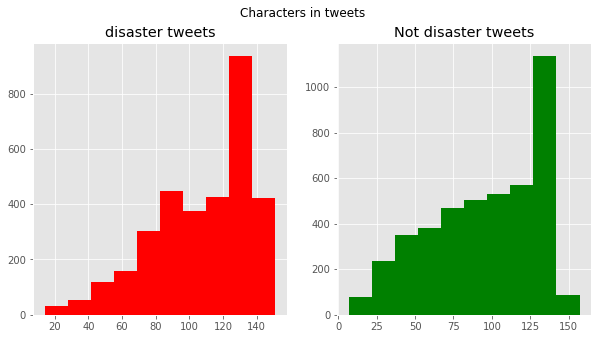
\includegraphics[width=\textwidth]{figures/LSTM2.png}
        \caption{推文中的字符数分布}
        \label{fig:char_dist}
    \end{subfigure}
    \hfill
    \begin{subfigure}[b]{0.48\textwidth}
        \centering
        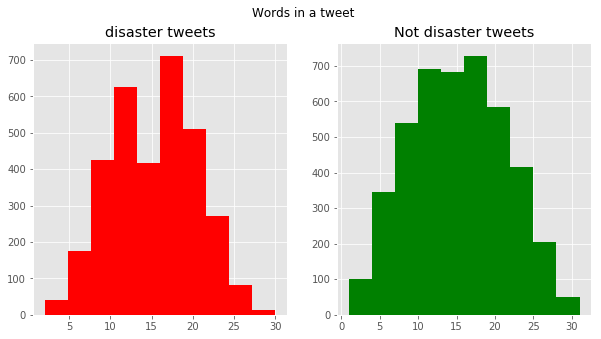
\includegraphics[width=\textwidth]{figures/LSTM3.png}
        \caption{推文中的词数分布}
        \label{fig:word_dist}
    \end{subfigure}
    \vspace{1cm}
    \begin{subfigure}[b]{0.48\textwidth}
        \centering
        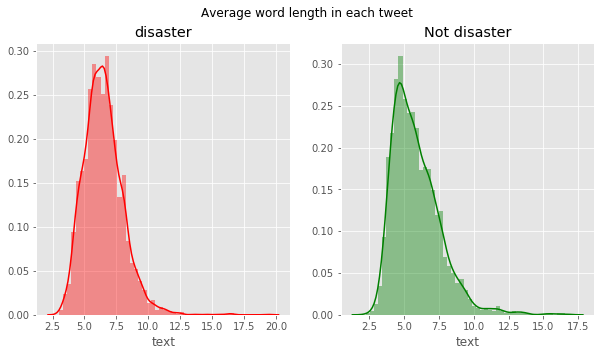
\includegraphics[width=\textwidth]{figures/LSTM4.png}
        \caption{推文中平均词长分布}
        \label{fig:avg_word_len}
    \end{subfigure}
    \caption{灾难性与非灾难性推文的基础文本统计对比}
    \label{fig:lstm_eda_basic}
\end{figure}

进一步地,我们分析了停用词(Stopwords)和标点符号的使用频率,如图 \ref{fig:lstm_eda_stop_punct} 所示。这些分析可以指导我们进行数据清洗和预处理,例如是否需要移除停用词和标点。
\begin{figure}[H]
    \centering
    \begin{subfigure}[b]{0.48\textwidth}
        \centering
        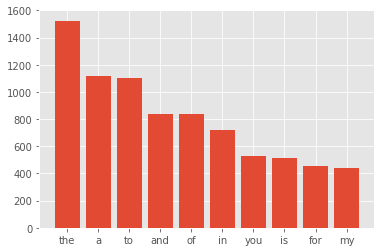
\includegraphics[width=\textwidth]{figures/LSTM5.png}
        \caption{非灾难性推文中的停用词}
        \label{fig:stopword_non_disaster}
    \end{subfigure}
    \hfill
    \begin{subfigure}[b]{0.48\textwidth}
        \centering
        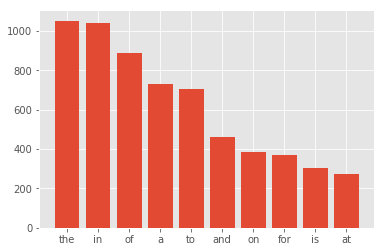
\includegraphics[width=\textwidth]{figures/LSTM6.png}
        \caption{灾难性推文中的停用词}
        \label{fig:stopword_disaster}
    \end{subfigure}
    
    \vspace{1cm}
    
    \begin{subfigure}[b]{0.48\textwidth}
        \centering
        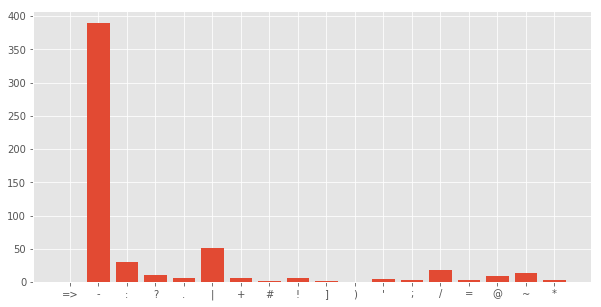
\includegraphics[width=\textwidth]{figures/LSTM7.png}
        \caption{灾难性推文中的标点符号}
        \label{fig:punct_disaster}
    \end{subfigure}
    \hfill
    \begin{subfigure}[b]{0.48\textwidth}
        \centering
        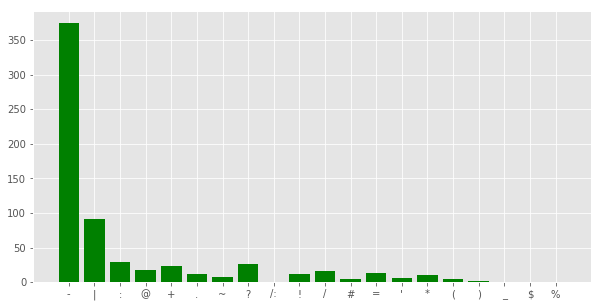
\includegraphics[width=\textwidth]{figures/LSTM8.png}
        \caption{非灾难性推文中的标点符号}
        \label{fig:punct_non_disaster}
    \end{subfigure}
    \caption{灾难性与非灾难性推文中停用词与标点符号的对比分析}
    \label{fig:lstm_eda_stop_punct}
\end{figure}

最后,通过分析最常见词汇和双词组合(Bigrams),如图 \ref{fig:lstm_eda_content},我们可以洞察两类推文在内容上的核心差异,这为特征工程和模型训练提供了重要依据。
\begin{figure}[H]
    \centering
    \begin{subfigure}[b]{0.48\textwidth}
        \centering
        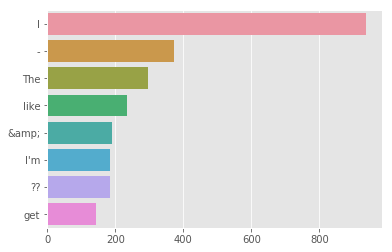
\includegraphics[width=\textwidth]{figures/LSTM9.png}
        \caption{常见词汇分析}
        \label{fig:common_words}
    \end{subfigure}
    \hfill
    \begin{subfigure}[b]{0.48\textwidth}
        \centering
        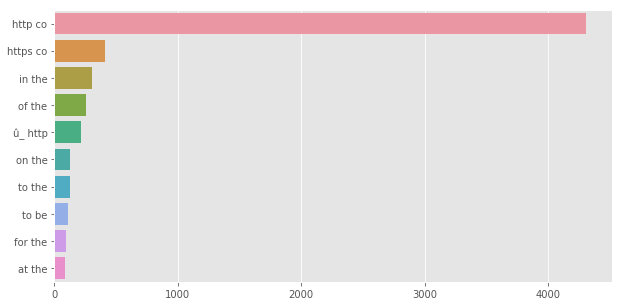
\includegraphics[width=\textwidth]{figures/LSTM10.png}
        \caption{常见双词组合(Bigrams)分析}
        \label{fig:common_bigrams}
    \end{subfigure}
    \caption{推文中内容词汇的频率分析}
    \label{fig:lstm_eda_content}
\end{figure}


\subsection{Transformer架构与自注意力机制}
\label{ssec:transformer}
2017年提出的Transformer 架构彻底改变了自然语言处理(NLP)领域。其核心创新是完全抛弃了RNN的循环结构,转而完全依赖于自注意力机制(Self-Attention Mechanism)。
\begin{itemize}
    \item \textbf{自注意力机制:}自注意力机制允许模型在处理一个序列时,直接计算序列中任意两个位置之间的依赖关系,而无需考虑它们之间的距离。对于序列中的每一个词,模型都会计算它与序列中所有其他词的“注意力分数”,这些分数决定了在编码当前词时,应该给予其他词多大的权重。这使得模型能够捕捉到句子内部复杂的语法和语义关系。
    \item \textbf{并行化优势:}由于摆脱了RNN的顺序计算依赖,Transformer 可以对整个序列进行并行计算,极大地提高了训练效率。
    \item \textbf{里程碑模型:}基于Transformer架构,诞生了一系列颠覆性的预训练语言模型,如BERT(Bidirectional Encoder Representations from Transformers)和GPT (Generative Pre-trained Transformer)系列。这些模型通过在海量无标注文本上进行预训练,学习到丰富的语言知识,然后在各种下游NLP任务上进行微调,取得了前所未有的性能表现。
\end{itemize}

\subsubsection*{案例研究:Transformer的内部工作原理}
\label{sssec:transformer_case_study}
为了更深入地剖析其内部机制,我们以一个Encoder-Decoder结构的Transformer为例,逐步拆解其核心组件。

\paragraph{1. 输入向量化与Q、K、V矩阵}
模型的第一步是将每个输入词的词嵌入(Embedding)向量,通过乘以三个可学习的权重矩阵 $W^Q, W^K, W^V$,分别转换为查询向量(Query)、键向量(Key)和值向量(Value)。如图 \ref{fig:qkv_creation} 所示,这些向量是计算自注意力的基础。
\begin{figure}[H]
    \centering
    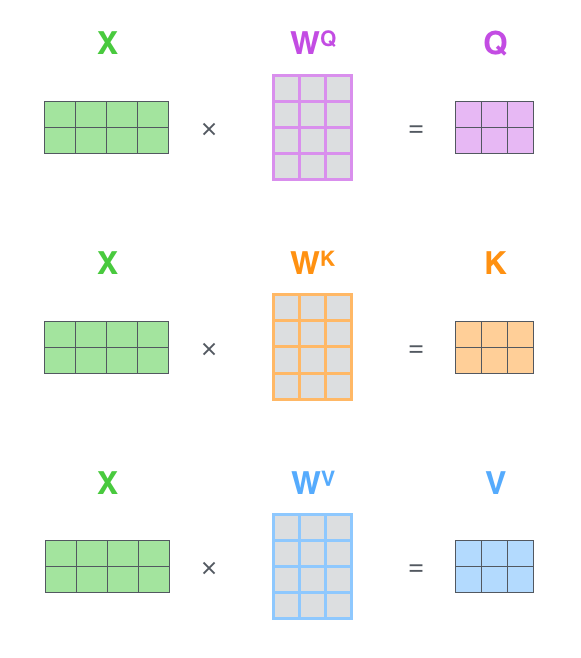
\includegraphics[width=0.7\textwidth]{figures/T1.png}
    \caption{从词嵌入向量X生成查询(Q)、键(K)、值(V)矩阵}
    \label{fig:qkv_creation}
\end{figure}

\paragraph{2. 缩放点积注意力(Scaled Dot-Product Attention)}
自注意力的核心计算遵循一个特定的公式,即缩放点积注意力,如图 \ref{fig:scaled_dot_product} 所示。其数学表达式为:
$$ \text{Attention}(Q, K, V) = \text{softmax}\left(\frac{QK^T}{\sqrt{d_k}}\right)V $$
这个公式的计算过程是:首先计算查询向量 $Q$ 与所有键向量 $K$ 的点积,然后除以一个缩放因子 $\sqrt{d_k}$($d_k$是键向量的维度)以稳定梯度,接着通过一个Softmax函数将结果归一化为注意力权重,最后将这些权重应用于值向量 $V$ 进行加权求和,得到该位置的注意力输出。
\begin{figure}[H]
    \centering
    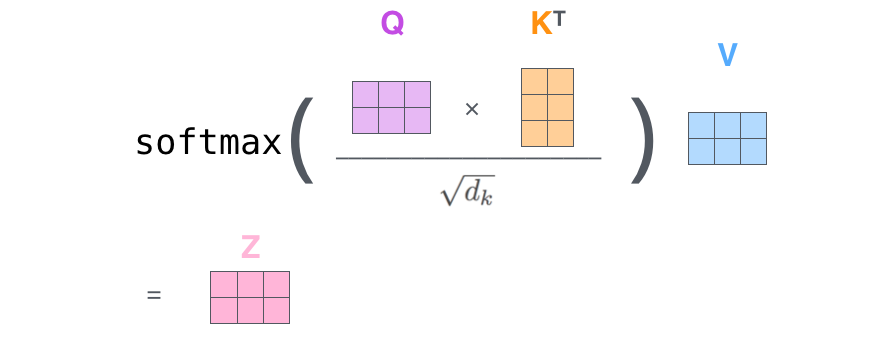
\includegraphics[width=0.6\textwidth]{figures/T2.png}
    \caption{缩放点积注意力的计算流程}
    \label{fig:scaled_dot_product}
\end{figure}

\paragraph{3. 多头注意力机制(Multi-Head Attention)}
为了让模型能够同时关注来自不同表示子空间的信息,Transformer采用了多头注意力机制。如图 \ref{fig:multi_head_overview} 和 \ref{fig:multi_head_concat} 所示,它将Q、K、V矩阵在维度上分割成多个“头”(Heads),对每个头独立地执行缩放点积注意力计算,然后将所有头的输出结果拼接(Concatenate)起来,并通过一个最终的权重矩阵 $W^O$ 进行线性变换,得到最终的输出。
\begin{figure}[H]
    \centering
    \begin{subfigure}[b]{0.48\textwidth}
        \centering
        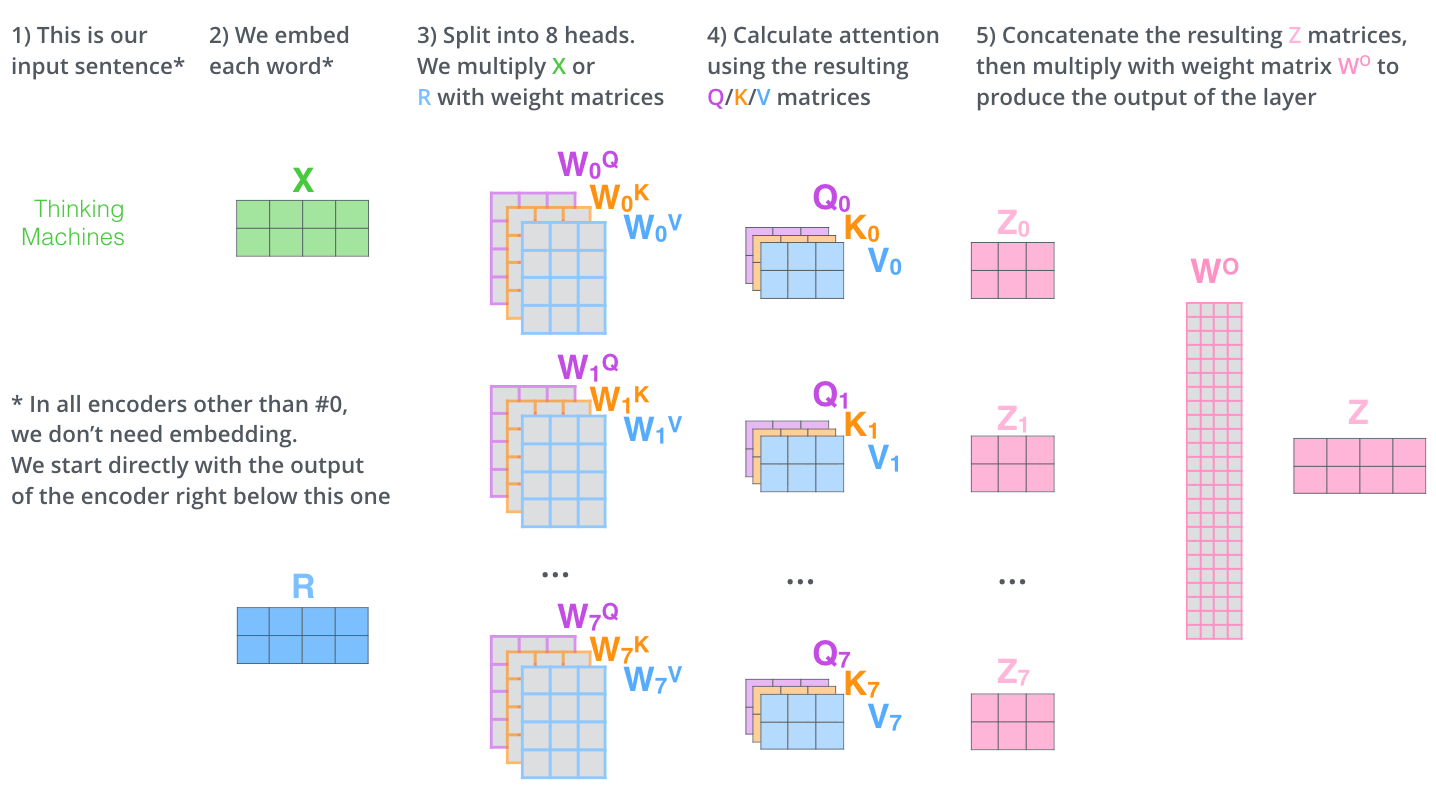
\includegraphics[width=\textwidth]{figures/T3.png}
        \caption{多头注意力机制概览}
        \label{fig:multi_head_overview}
    \end{subfigure}
    \hfill
    \begin{subfigure}[b]{0.48\textwidth}
        \centering
        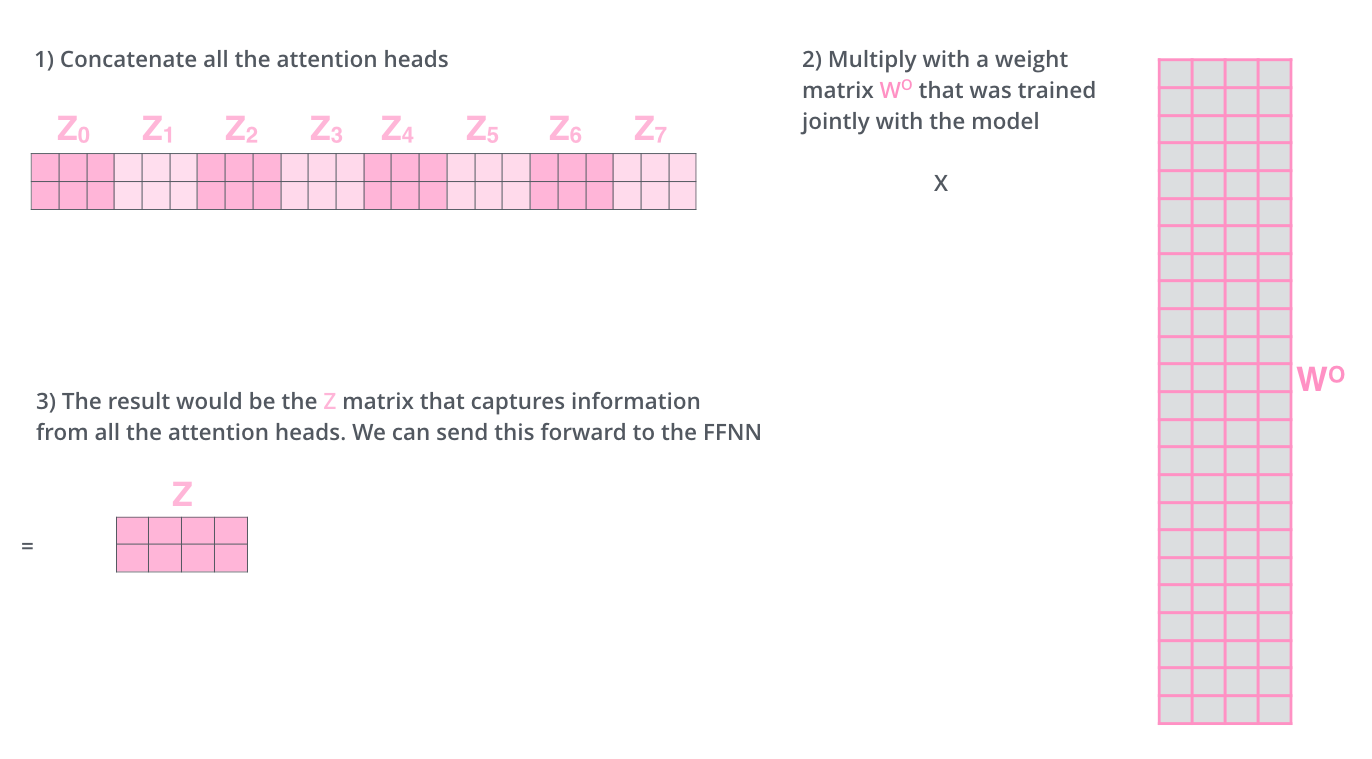
\includegraphics[width=\textwidth]{figures/T4.png}
        \caption{拼接多个注意力头的输出}
        \label{fig:multi_head_concat}
    \end{subfigure}
    \caption{多头注意力机制的分解与整合}
    \label{fig:multi_head_process}
\end{figure}

图 \ref{fig:self_attention_example} 直观地展示了自注意力机制的效果。在处理句子“The animal didn't cross the street because it was too tired”时,其中一个注意力头在编码单词“it”时,会将大部分的注意力分配给“animal”,从而正确地理解了“it”的指代对象。
\begin{figure}[H]
    \centering
    \begin{subfigure}[b]{0.48\textwidth}
        \centering
        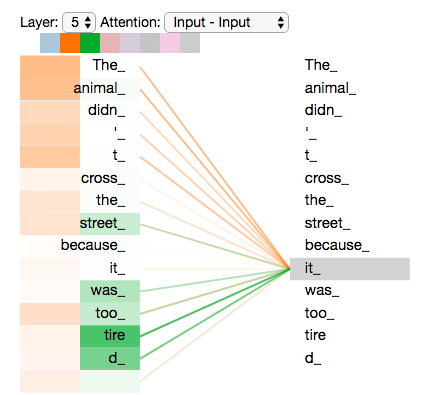
\includegraphics[width=\textwidth]{figures/T5.png}
        \caption{自注意力机制对“it”的指代分析(注意力头5)}
        \label{fig:self_attention_it_1}
    \end{subfigure}
    \hfill
    \begin{subfigure}[b]{0.48\textwidth}
        \centering
        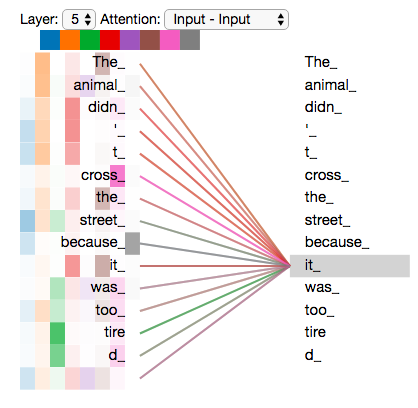
\includegraphics[width=\textwidth]{figures/T6.png}
        \caption{另一个注意力头对“it”的关注点}
        \label{fig:self_attention_it_2}
    \end{subfigure}
    \caption{自注意力机制的可视化实例对比}
    \label{fig:self_attention_example}
\end{figure}

\paragraph{4. 整体架构:编码器与解码器}
Transformer模型由编码器(Encoder)和解码器(Decoder)堆栈组成。每个编码器层(如图 \ref{fig:encoder_block})包含一个多头自注意力层和一个前馈神经网络层,并通过残差连接(Residual Connection)和层归一化(Layer Normalization)进行优化。解码器层则在编码器层的基础上,增加了一个用于处理编码器输出的“编码器-解码器注意力”层。整个架构如图 \ref{fig:transformer_architecture} 所示,最终通过一个线性和Softmax层输出预测结果的概率分布(如图 \ref{fig:final_output_layer})。
\begin{figure}[H]
    \centering
    \begin{subfigure}[b]{0.48\textwidth}
        \centering
        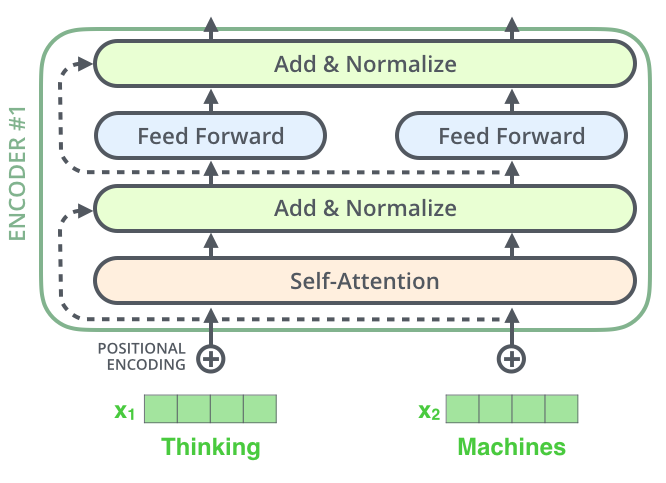
\includegraphics[width=\textwidth]{figures/T7.png}
        \caption{编码器(Encoder)层结构}
        \label{fig:encoder_block_1}
    \end{subfigure}
    \hfill
    \begin{subfigure}[b]{0.48\textwidth}
        \centering
        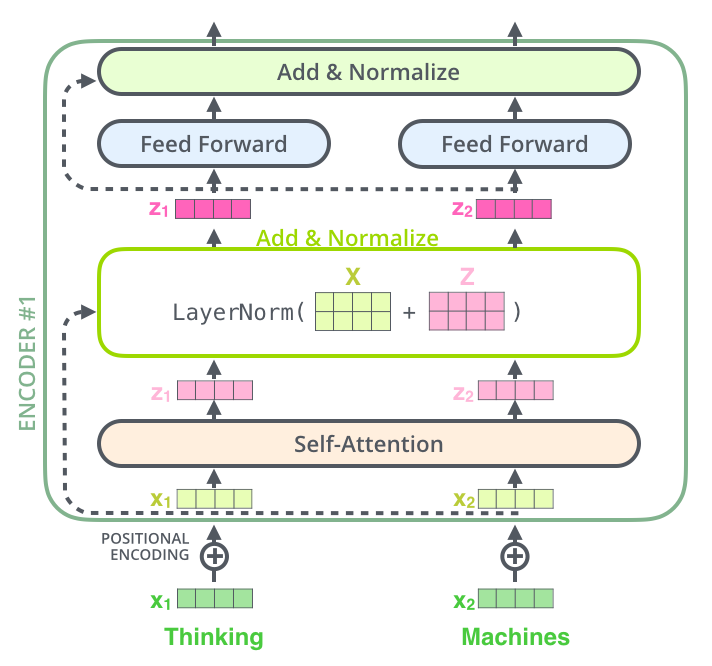
\includegraphics[width=\textwidth]{figures/T8.png}
        \caption{编码器中的Add \& Normalize细节}
        \label{fig:encoder_block_2}
    \end{subfigure}
    \caption{Transformer编码器模块结构}
    \label{fig:encoder_block}
\end{figure}

\begin{figure}[H]
    \centering
    \begin{subfigure}[b]{0.48\textwidth}
        \centering
        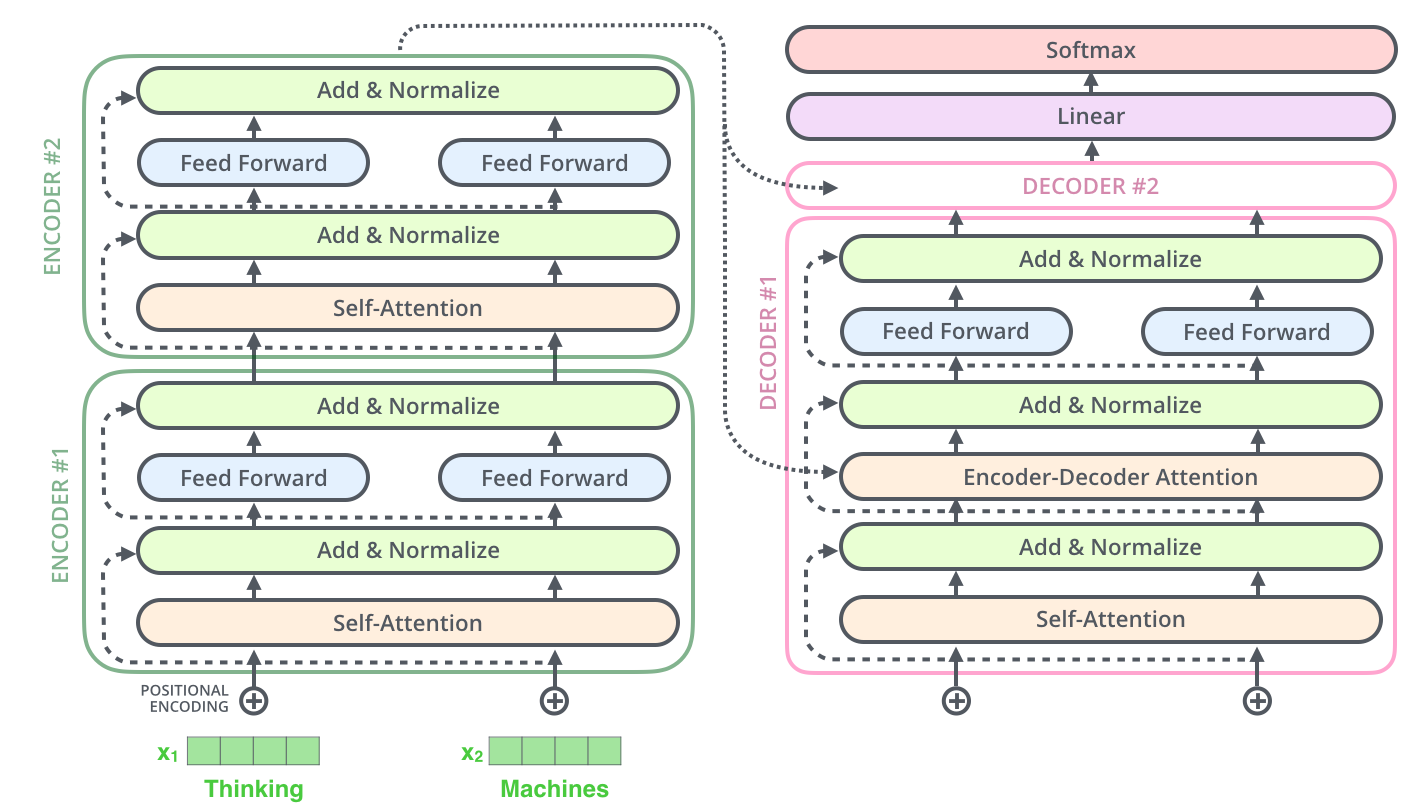
\includegraphics[width=\textwidth]{figures/T9.png}
        \caption{完整的Transformer模型架构}
        \label{fig:transformer_architecture}
    \end{subfigure}
    \hfill
    \begin{subfigure}[b]{0.48\textwidth}
        \centering
        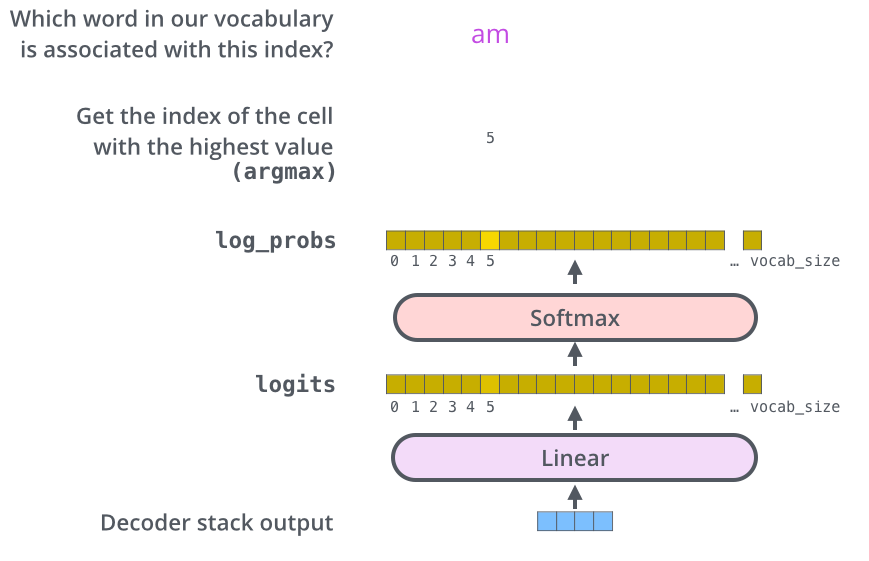
\includegraphics[width=\textwidth]{figures/T10.png}
        \caption{最终的线性和Softmax输出层}
        \label{fig:final_output_layer}
    \end{subfigure}
    \caption{Transformer整体架构与输出层}
    \label{fig:transformer_full_view}
\end{figure}

\section{生成式人工智能(Generative AI)}
\label{sec:generative_ai}
生成式人工智能旨在创造新的、原创性的内容,如图像、文本、音乐和代码,而非仅仅进行分类或预测。
\begin{itemize}
    \item \textbf{生成对抗网络(GANs):} 生成对抗网络(Generative Adversarial Networks, GANs)由一个生成器(Generator)和一个判别器(Discriminator)组成。生成器的任务是生成以假乱真的数据(如图片),而判别器的任务是尽可能准确地分辨出哪些数据是真实的,哪些是生成器伪造的。两者通过一种“对抗游戏”的方式进行训练:生成器努力欺骗判别器,而判别器则努力不被欺骗。这种对抗过程最终能驱动生成器产生高度逼真和多样化的内容。
    
    \subsubsection*{案例研究:GAN的博弈过程与训练细节}
    \label{sssec:gan_case_study}
    GAN 的核心思想是通过生成器(Generator, $G$)和判别器(Discriminator, $D$)之间的“对抗”来学习数据的真实分布。我们可以将 $D$ 视作一个传统的分类器(如图 \ref{fig:gan_discriminator_model}),其任务是判断输入是真实数据还是伪造数据;而 $G$ 则是一个生成模型(如图 \ref{fig:gan_generative_model}),它试图将简单的随机噪声 $z$ 映射为与真实数据无法区分的样本 $G(z)$ \cite{15}。

    \begin{figure}[H]
        \centering
        \begin{subfigure}[b]{0.48\textwidth}
            \centering
            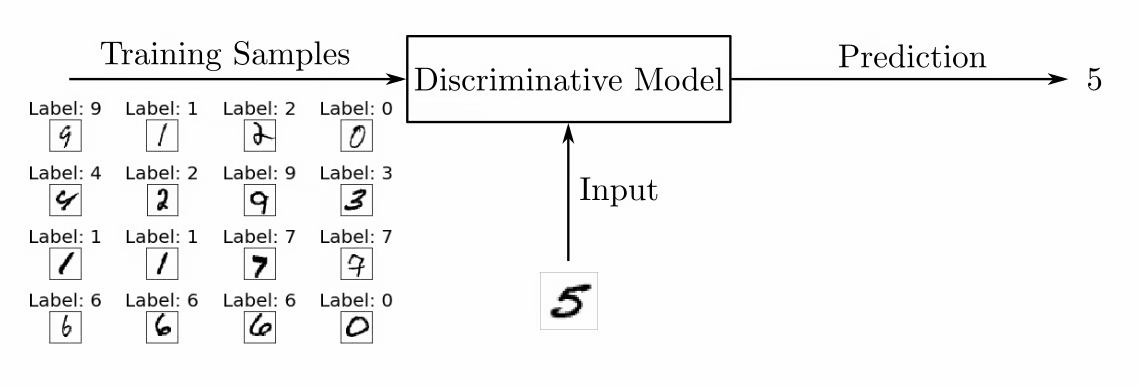
\includegraphics[width=\textwidth]{figures/GAN1.png}
            \caption{判别模型(Discriminative Model)示意图}
            \label{fig:gan_discriminator_model}
        \end{subfigure}
        \hfill
        \begin{subfigure}[b]{0.48\textwidth}
            \centering
            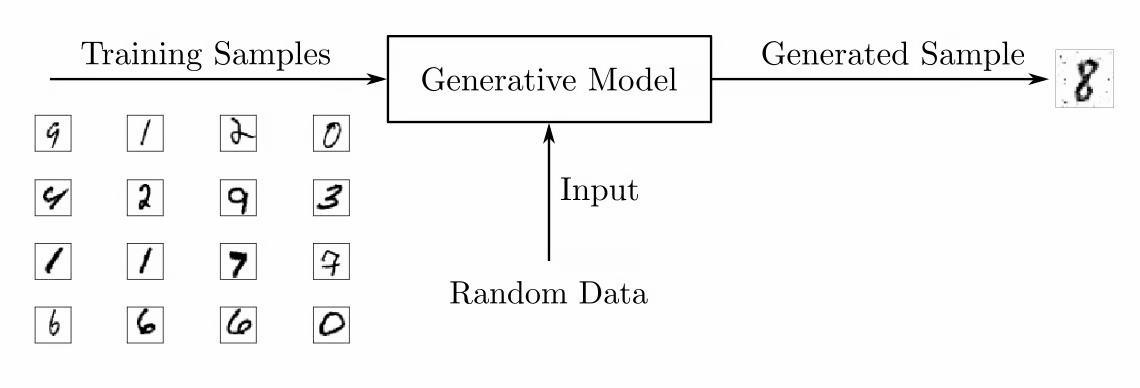
\includegraphics[width=\textwidth]{figures/GAN2.png}
            \caption{生成模型(Generative Model)示意图}
            \label{fig:gan_generative_model}
        \end{subfigure}
        \caption{GAN的两个核心组件:判别器与生成器}
        \label{fig:gan_components}
    \end{figure}

    \paragraph{1. 训练过程的数学解析}
    GAN的训练过程是一个迭代的、分阶段的博弈,其整体流程如图 \ref{fig:gan_full_training_loop} 所示。

    \begin{figure}[H]
        \centering
        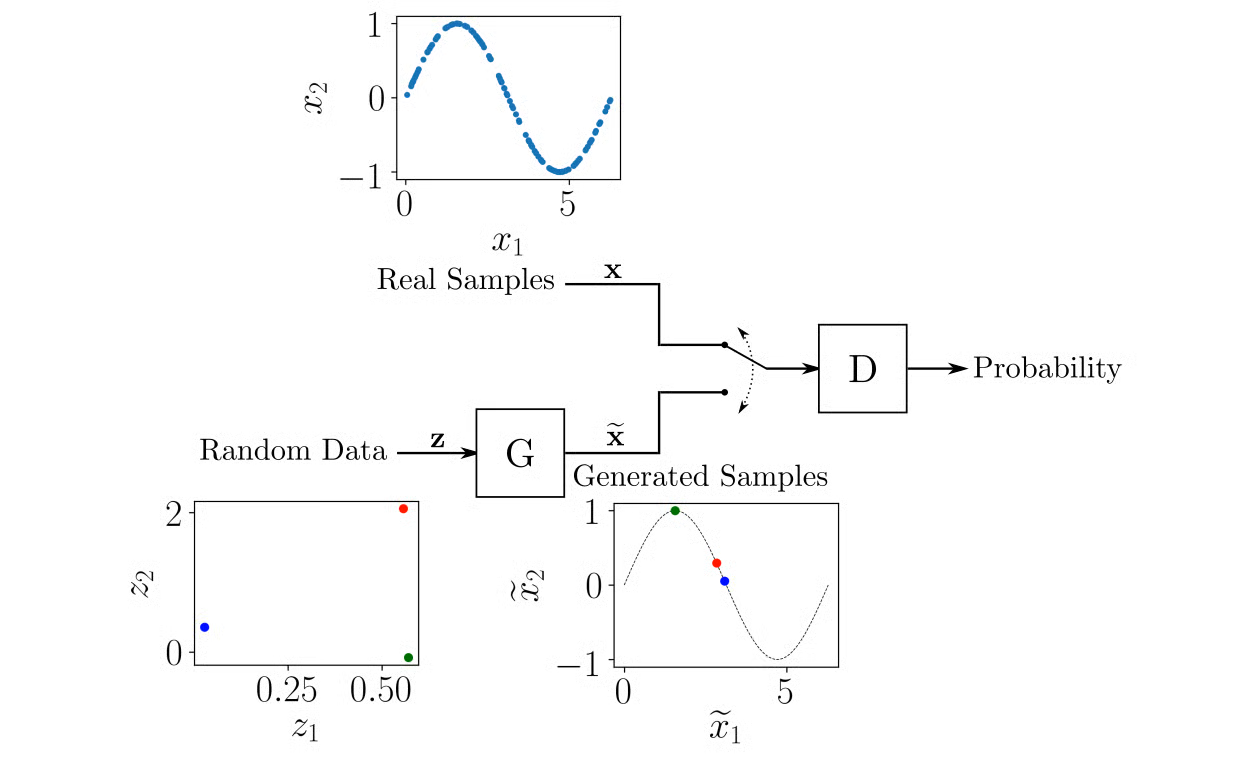
\includegraphics[width=0.9\textwidth]{figures/GAN4.png}
        \caption{GAN的整体训练循环示意图,展示了从真实样本(Real Samples)和生成样本(Generated Samples)到判别器和损失函数的完整流程}
        \label{fig:gan_full_training_loop}
    \end{figure}
    
    这个过程在数学上可以分解为两个独立的优化阶段(如图 \ref{fig:gan_training_phases}):
    \begin{itemize}
        \item \textbf{阶段一:训练判别器 $D$。} 在此阶段,生成器 $G$ 的参数被固定。判别器 $D$ 的目标是最大化其正确分类的能力,即对于来自真实数据分布 $p_{\text{data}}(x)$ 的样本 $x$,最大化 $D(x)$;对于来自生成器 $G$ 的伪造样本 $G(z)$(其中 $z \sim p_z(z)$),最大化 $1 - D(G(z))$ \cite{15}。这等价于最大化以下目标函数,也就是之前提到的价值函数 $V(D,G)$:
        $$ \max_{D} V(D, G) = \mathbb{E}_{x \sim p_{\text{data}}(x)}[\log D(x)] + \mathbb{E}_{z \sim p_{z}(z)}[\log(1 - D(G(z)))] $$
        
        \item \textbf{阶段二:训练生成器 $G$。} 判别器 $D$ 的参数被固定。生成器 $G$ 的目标是最小化其生成样本被判别器识别出来的概率,即最小化 $1 - D(G(z))$,这等价于最大化 $D(G(z))$ \cite{15}。在实践中,为了避免在训练初期因 $D$ 过强而导致 $G$ 的梯度消失问题,通常不直接最小化 $\log(1 - D(G(z)))$,而是采用非饱和的目标函数,即最大化 $\log D(G(z))$ \cite{15}。因此,生成器的优化目标是:
        $$ \max_{G} V_G = \mathbb{E}_{z \sim p_{z}(z)}[\log D(G(z))] $$
    \end{itemize}
    
    \begin{figure}[H]
        \centering
        \begin{subfigure}[b]{0.48\textwidth}
            \centering
            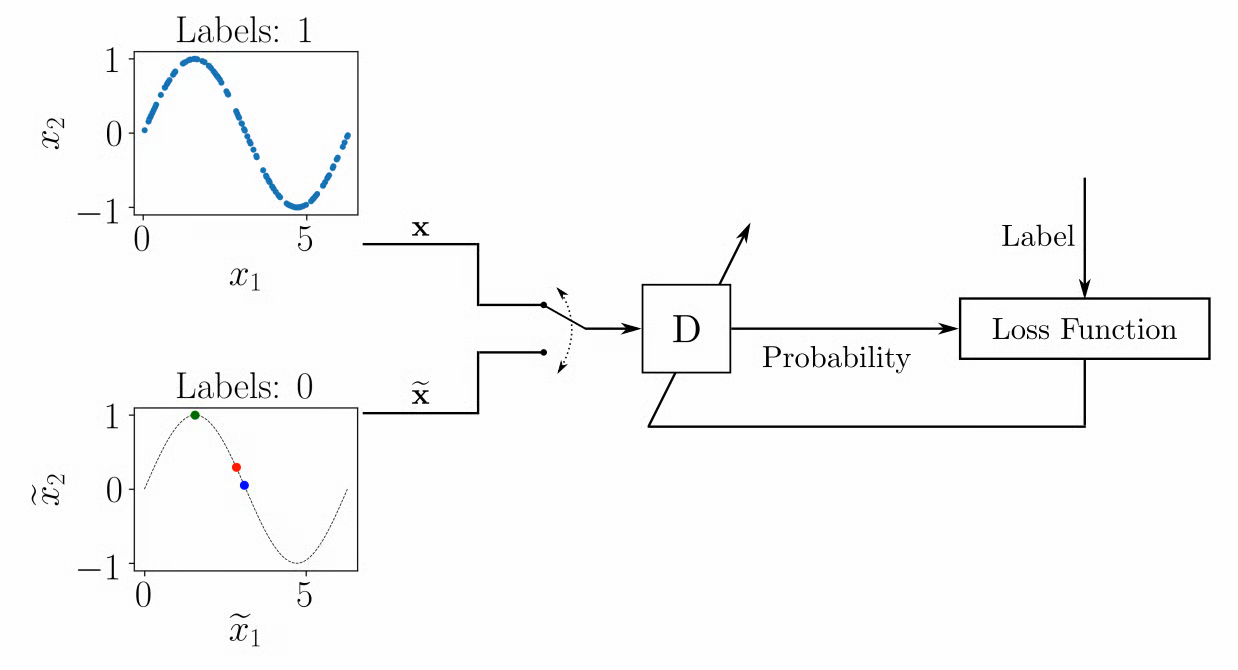
\includegraphics[width=\textwidth]{figures/GAN5.png}
            \caption{训练判别器D的阶段:固定G,优化D以区分真伪样本。真实样本x的标签为1,生成样本G(z)的标签为0。}
            \label{fig:gan_train_discriminator}
        \end{subfigure}
        \hfill
        \begin{subfigure}[b]{0.48\textwidth}
            \centering
            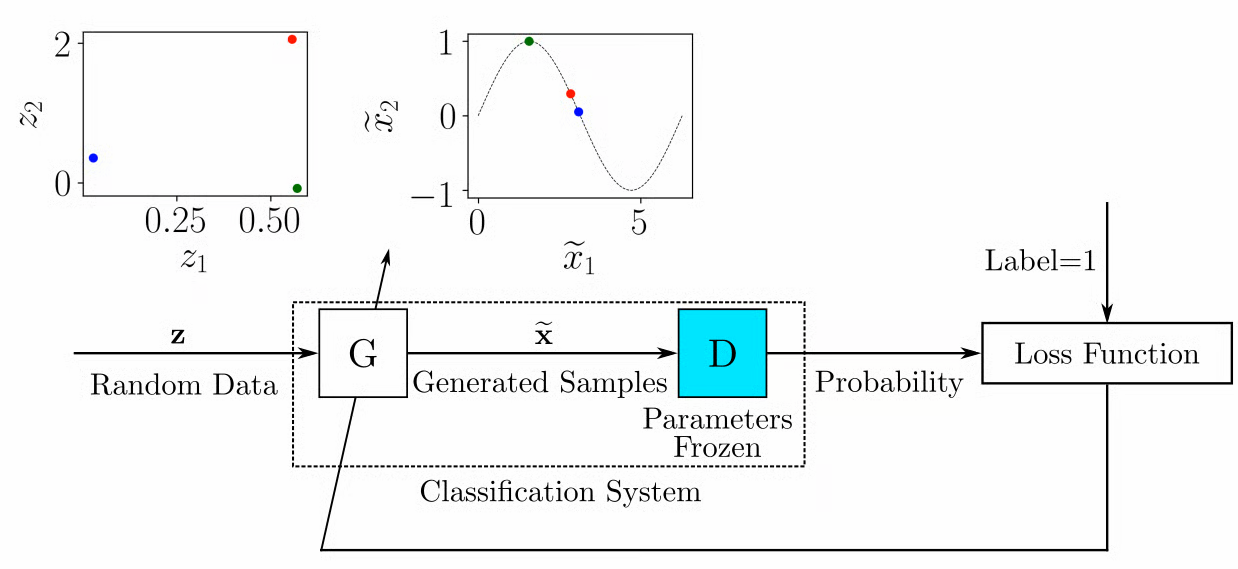
\includegraphics[width=\textwidth]{figures/GAN6.png}
            \caption{训练生成器G的阶段:固定D,优化G以生成能让D判断为“真”(标签1)的样本。}
            \label{fig:gan_train_generator}
        \end{subfigure}
        \caption{GAN训练的两个交替阶段对比}
        \label{fig:gan_training_phases}
    \end{figure}

    \paragraph{2. 收敛与理论最优解}
    当且仅当生成分布 $p_g$ 与真实数据分布 $p_{\text{data}}$ 完全一致时,这个博弈过程达到纳什均衡 \cite{89}。此时,判别器 $D$ 无法区分真实样本与生成样本,对于任何输入 $x$,其输出概率恒为 $\frac{1}{2}$ ,即:
    $$ D_{G}^{*}(x) = \frac{p_{\text{data}}(x)}{p_{\text{data}}(x) + p_{g}(x)} = \frac{1}{2} $$
    从理论上,这个过程等价于最小化真实分布与生成分布之间的JS散度(Jensen-Shannon Divergence),这为GAN的收敛性提供了理论保障 \cite{90}。
    
    \paragraph{3. GAN的架构与应用实例}
    现代GAN,特别是深度卷积生成对抗网络(DCGAN),使用深度卷积网络作为生成器和判别器的架构。生成器通常由一系列转置卷积(或称反卷积)层构成,将一个低维的随机噪声向量 $z$ 逐步上采样,最终生成高分辨率的图像(如图 \ref{fig:dcgan_generator_arch} 所示)。通过学习,GAN能够捕捉到数据背后的复杂流形结构,将简单的噪声分布(如图 \ref{fig:gan_manifold_learning} 中的Samples)映射为具有丰富细节的生成图像。

    \begin{figure}[H]
        \centering
        \begin{subfigure}[b]{0.48\textwidth}
            \centering
            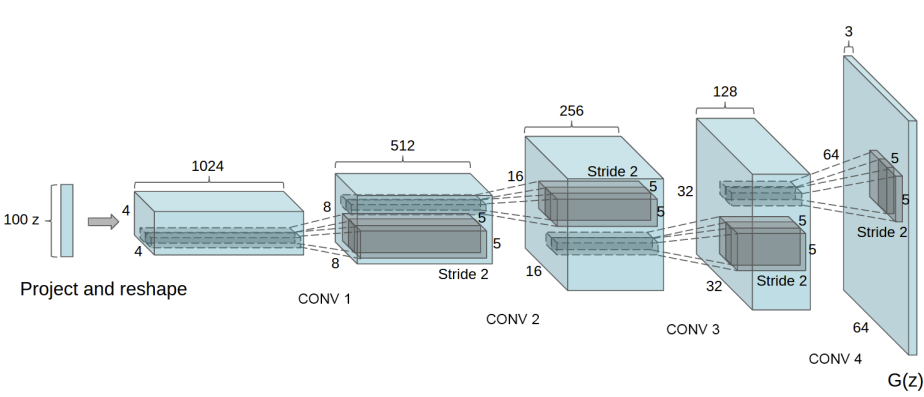
\includegraphics[width=\textwidth]{figures/GAN7.png}
            \caption{一个典型的DCGAN生成器网络结构}
            \label{fig:dcgan_generator_arch}
        \end{subfigure}
        \hfill
        \begin{subfigure}[b]{0.48\textwidth}
            \centering
            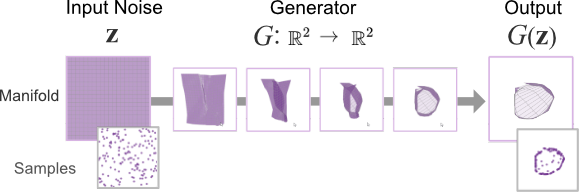
\includegraphics[width=\textwidth]{figures/GAN8.png}
            \caption{GAN学习数据流形的可视化过程}
            \label{fig:gan_manifold_learning}
        \end{subfigure}
        \caption{DCGAN架构示例与GAN的流形学习能力}
        \label{fig:gan_arch_and_manifold}
    \end{figure}

    \item \textbf{扩散模型(Diffusion Models):} 扩散模型是近年来在图像生成领域取得巨大成功的另一类生成模型。其核心思想分为两个过程:一个前向的“扩散”过程和一个反向的“去噪”过程。在前向过程中,模型逐步地向一张真实的图片中添加噪声,直到其完全变为纯噪声。在反向过程中,模型学习如何从纯噪声开始,逐步地、迭代地去除噪声,最终恢复出一张清晰、高质量的图片。正是通过学习这个去噪过程,模型掌握了生成新图像的能力。

    \subsubsection*{案例研究:扩散模型的数学原理与实现}
    \label{sssec:diffusion_case_study}
    扩散模型(Denoising Diffusion Probabilistic Models, DDPMs)通过模拟一个逐渐破坏数据再重建数据的过程来进行学习和生成 \cite{croitoru2023diffusion}。

    \paragraph{1. 前向过程(Forward Process / Diffusion Process)}
    前向过程是一个固定的马尔可夫链,它逐步地向原始数据 $x_0$(来自真实数据分布 $q(x_0)$)中添加高斯噪声。这个过程持续 $T$ 个时间步,噪声的方差由一个预设的时间表(variance schedule)$\{\beta_t\}_{t=1}^T$ 控制。在任意时间步 $t$,从 $x_{t-1}$ 到 $x_t$ 的转换被定义为:
    $$ q(x_t | x_{t-1}) = \mathcal{N}(x_t; \sqrt{1 - \beta_t} x_{t-1}, \beta_t \mathbf{I}) $$
    如图 \ref{fig:diffusion_forward_process} 所示,随着 $t$ 的增加,数据逐渐失去其原有特征,最终在 $t=T$ 时近似于一个标准高斯分布 $\mathcal{N}(0, \mathbf{I})$。这个过程的一个重要特性是,我们可以通过以下公式直接从原始数据 $x_0$ 采样任意时间步 $t$ 的含噪数据 $x_t$:
    $$ q(x_t | x_0) = \mathcal{N}(x_t; \sqrt{\bar{\alpha}_t} x_0, (1 - \bar{\alpha}_t) \mathbf{I}) $$
    其中 $\alpha_t = 1 - \beta_t$ 且 $\bar{\alpha}_t = \prod_{i=1}^t \alpha_i$。

    \begin{figure}[H]
        \centering
        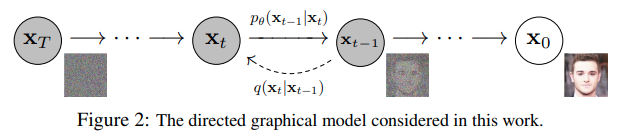
\includegraphics[width=\textwidth]{figures/D1.png}
        \caption{扩散模型的前向过程:从清晰图像($x_0$)逐步添加噪声,直至变为纯噪声图像($x_T$)。}
        \label{fig:diffusion_forward_process}
    \end{figure}

    \paragraph{2. 反向过程(Reverse Process / Denoising Process)}
    反向过程的目标是学习前向过程的逆过程,即从纯噪声 $x_T$ 中逐步去除噪声,最终恢复出原始数据 $x_0$。这个过程也是一个马尔可夫链,但其转移概率是未知的,需要通过一个深度神经网络(通常是U-Net架构)来学习。我们将这个由参数 $\theta$ 控制的神经网络表示为 $p_\theta$。反向过程的每一步定义为:
    $$ p_\theta(x_{t-1} | x_t) = \mathcal{N}(x_{t-1}; \mu_\theta(x_t, t), \Sigma_\theta(x_t, t)) $$
    如图 \ref{fig:diffusion_reverse_process} 所示,模型在每个时间步 $t$ 预测噪声,然后从含噪图像 $x_t$ 中减去预测的噪声,得到一个更清晰的图像 $x_{t-1}$。
    
    \begin{figure}[H]
        \centering
        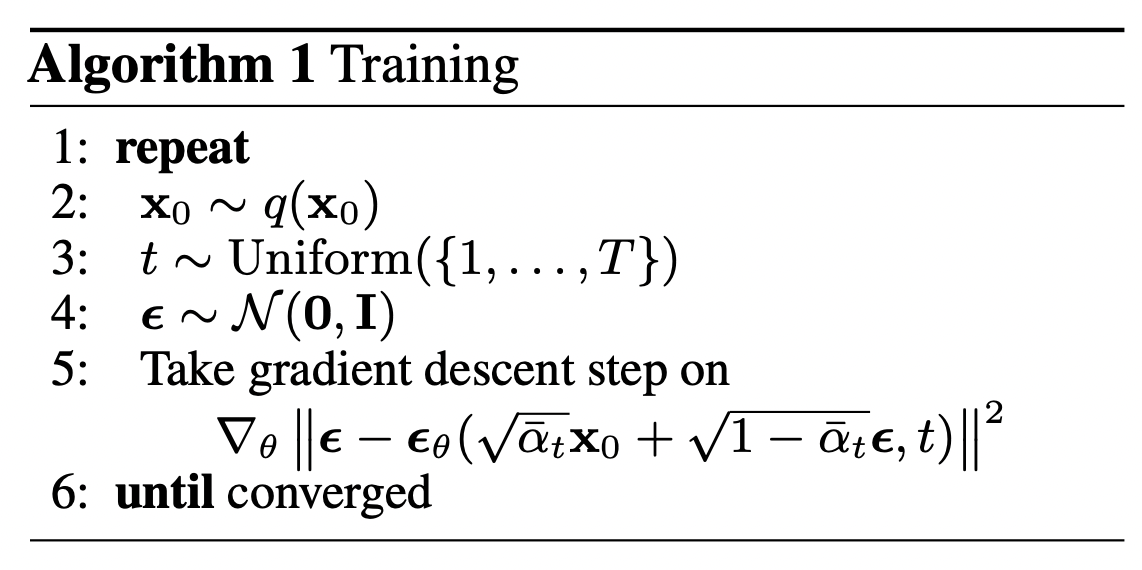
\includegraphics[width=\textwidth]{figures/D2.png}
        \caption{扩散模型的反向(去噪)过程:从随机噪声($x_T$)开始,由神经网络引导,逐步恢复出清晰图像($x_0$)。}
        \label{fig:diffusion_reverse_process}
    \end{figure}

    \paragraph{3. 训练目标与损失函数}
    扩散模型的训练目标是最大化数据的对数似然 $\log p_\theta(x_0)$。通过变分推断,这个目标可以转化为最小化一个损失函数 $L(\theta)$,该损失函数衡量了真实的反向过程后验概率 $q(x_{t-1} | x_t, x_0)$ 与模型学习到的近似后验概率 $p_\theta(x_{t-1} | x_t)$ 之间的KL散度 \cite{315}。经过简化,一个更直接的训练目标是让神经网络 $\epsilon_\theta(x_t, t)$ 在每个时间步都能准确地预测出添加到 $x_0$ 中以产生 $x_t$ 的噪声 $\epsilon$。其简化的损失函数为:
    $$ L_{\text{simple}}(\theta) = \mathbb{E}_{t, x_0, \epsilon} \left[ || \epsilon - \epsilon_\theta(\sqrt{\bar{\alpha}_t}x_0 + \sqrt{1 - \bar{\alpha}_t}\epsilon, t) ||^2 \right] $$
    其中 $t$ 从 $\{1, ..., T\}$ 中均匀采样,$\epsilon \sim \mathcal{N}(0, \mathbf{I})$。如图 \ref{fig:diffusion_training_objective} 所示,模型通过不断地比较真实噪声和预测噪声的差异来优化自身参数。
    
    \begin{figure}[H]
        \centering
        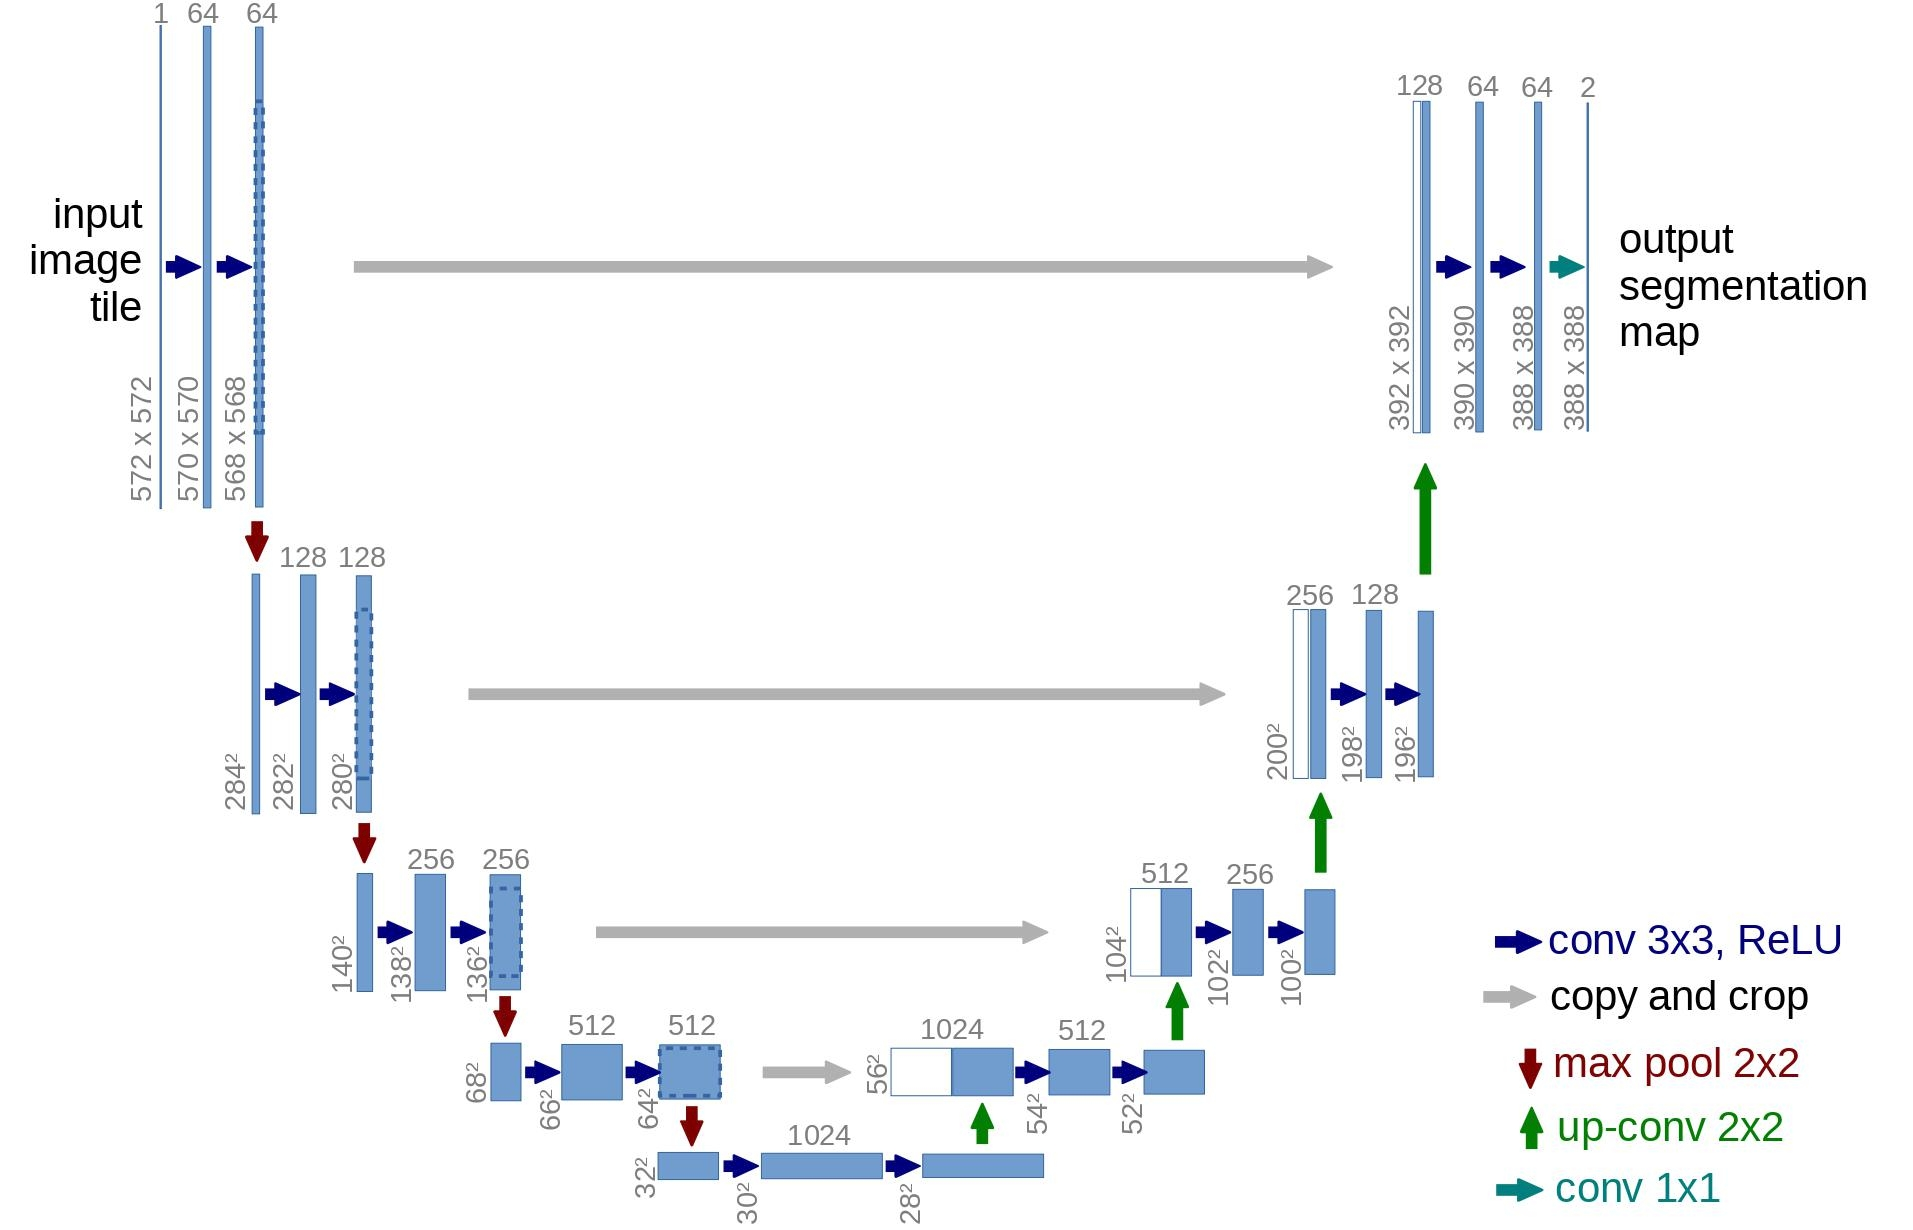
\includegraphics[width=0.8\textwidth]{figures/D3.png}
        \caption{扩散模型的训练目标:神经网络 $\epsilon_\theta$ 学习预测在时间步t添加到原始图像$x_0$上的噪声。}
        \label{fig:diffusion_training_objective}
    \end{figure}

    \paragraph{4. 架构与应用实例}
    扩散模型的生成能力在近年来的多个模型中得到了验证,如GLIDE, DALL-E 2, Imagen, 和Stable Diffusion等。这些模型通过在反向过程中引入额外的条件(如文本描述),实现了高质量的文本到图像生成。图 \ref{fig:diffusion_model_examples} 展示了不同扩散模型生成的图像,体现了其在生成细节丰富、语义准确的图像方面的强大能力。

    \begin{figure}[H]
        \centering
        \begin{subfigure}[b]{0.32\textwidth}
            \centering
            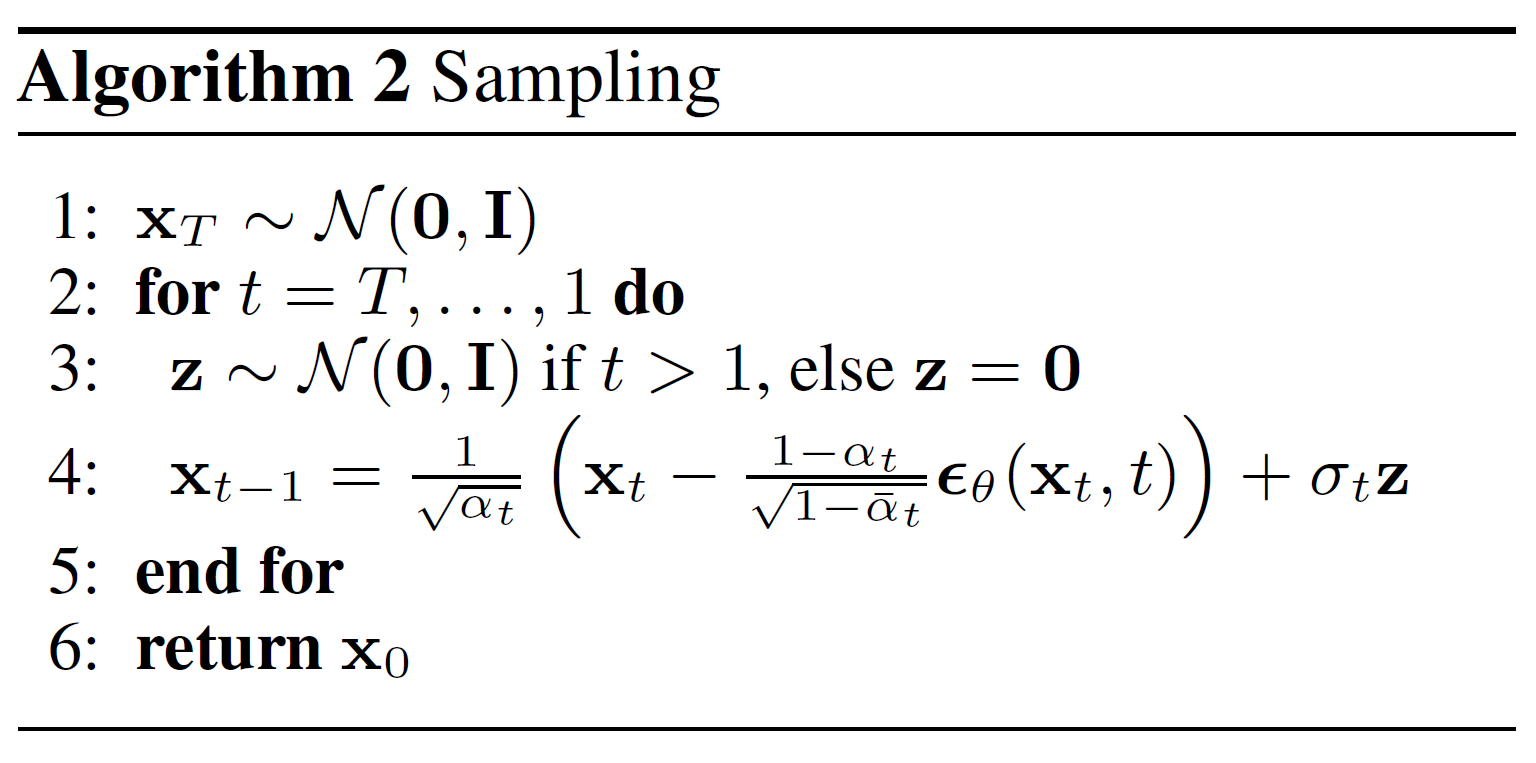
\includegraphics[width=\textwidth]{figures/D4.png}
            \caption{GLIDE}
            \label{fig:glide_example}
        \end{subfigure}
        \hfill
        \begin{subfigure}[b]{0.32\textwidth}
            \centering
            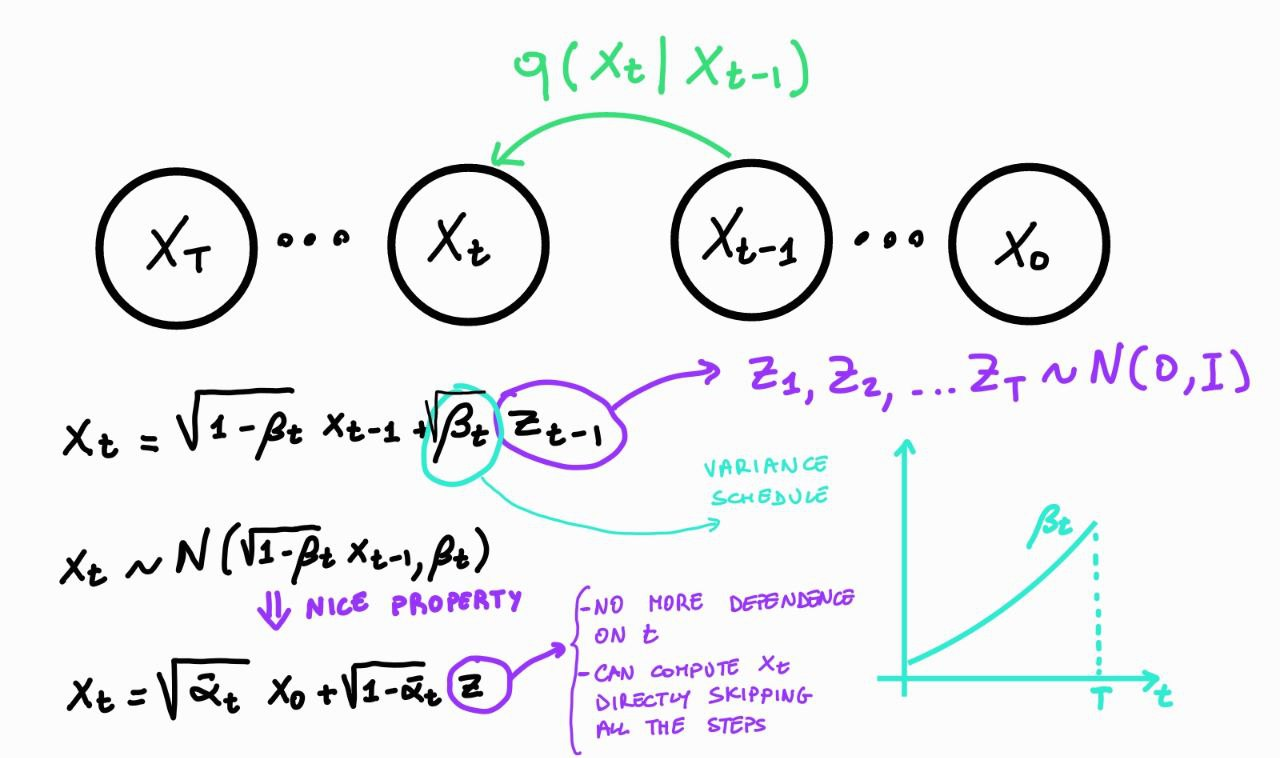
\includegraphics[width=\textwidth]{figures/D5.png}
            \caption{DALL-E 2}
            \label{fig:dalle2_example}
        \end{subfigure}
        \hfill
        \begin{subfigure}[b]{0.32\textwidth}
            \centering
            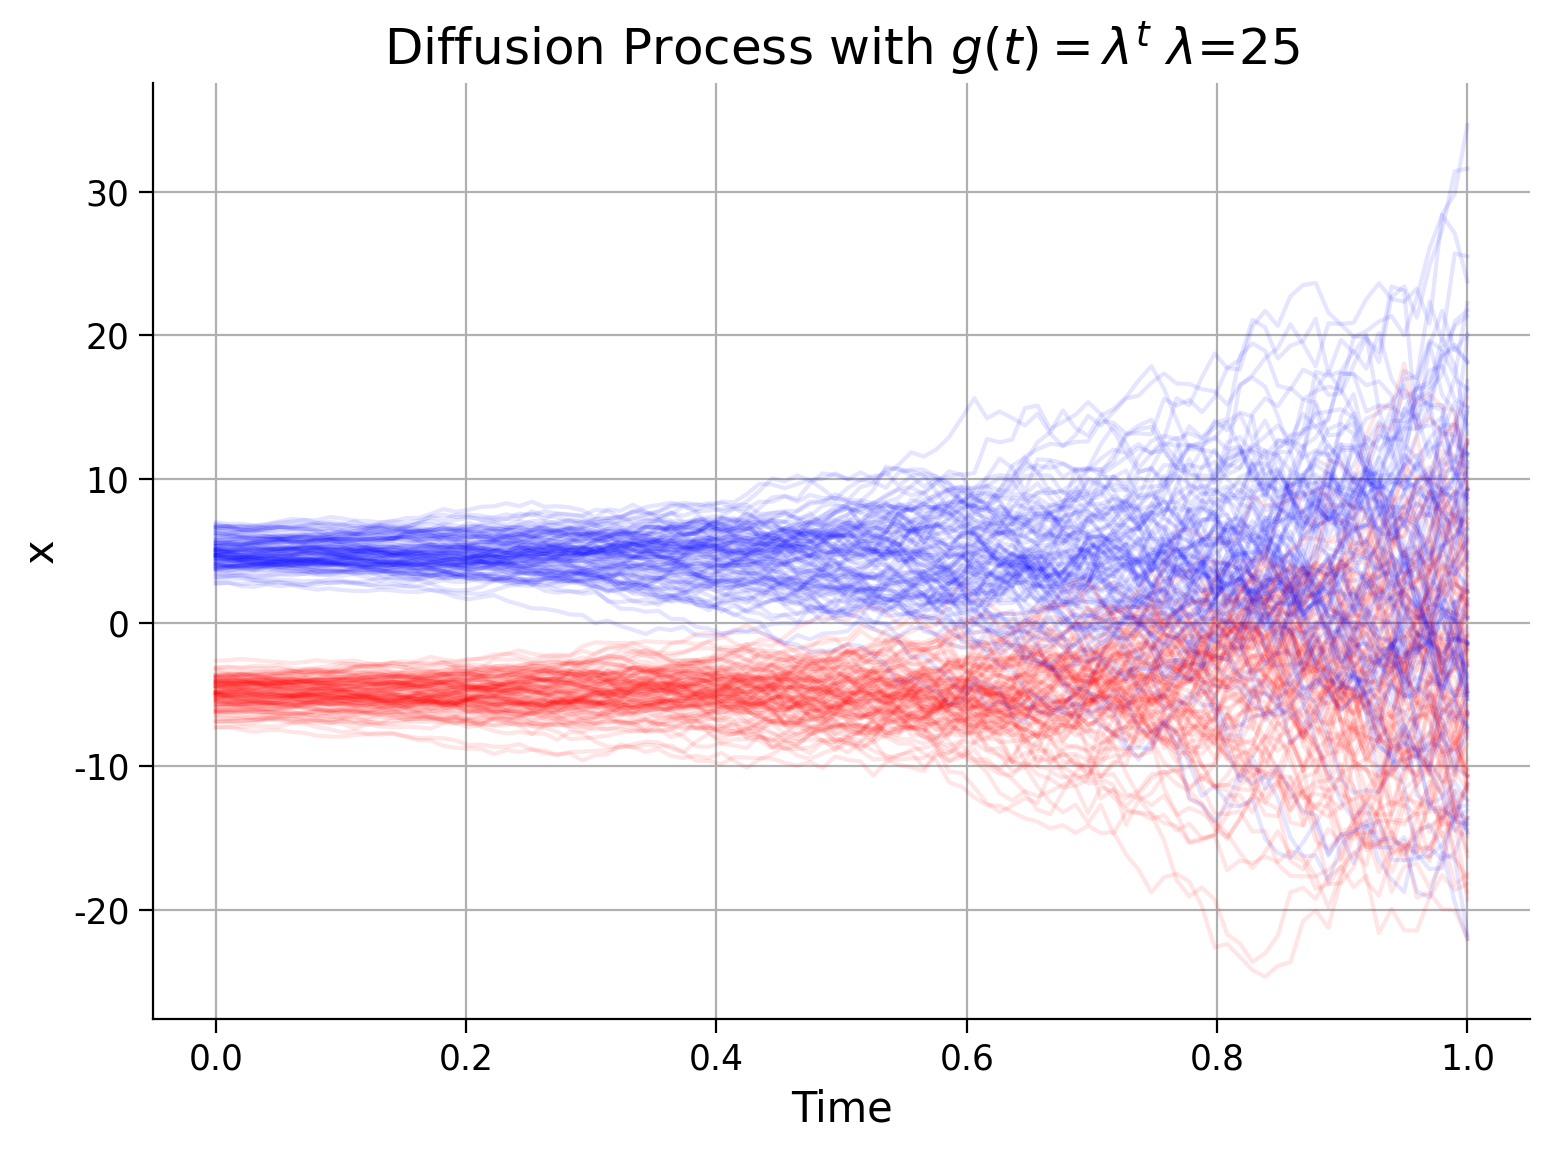
\includegraphics[width=\textwidth]{figures/D6.png}
            \caption{Imagen}
            \label{fig:imagen_example}
        \end{subfigure}
        
        \vspace{1cm}
        
        \begin{subfigure}[b]{0.48\textwidth}
            \centering
            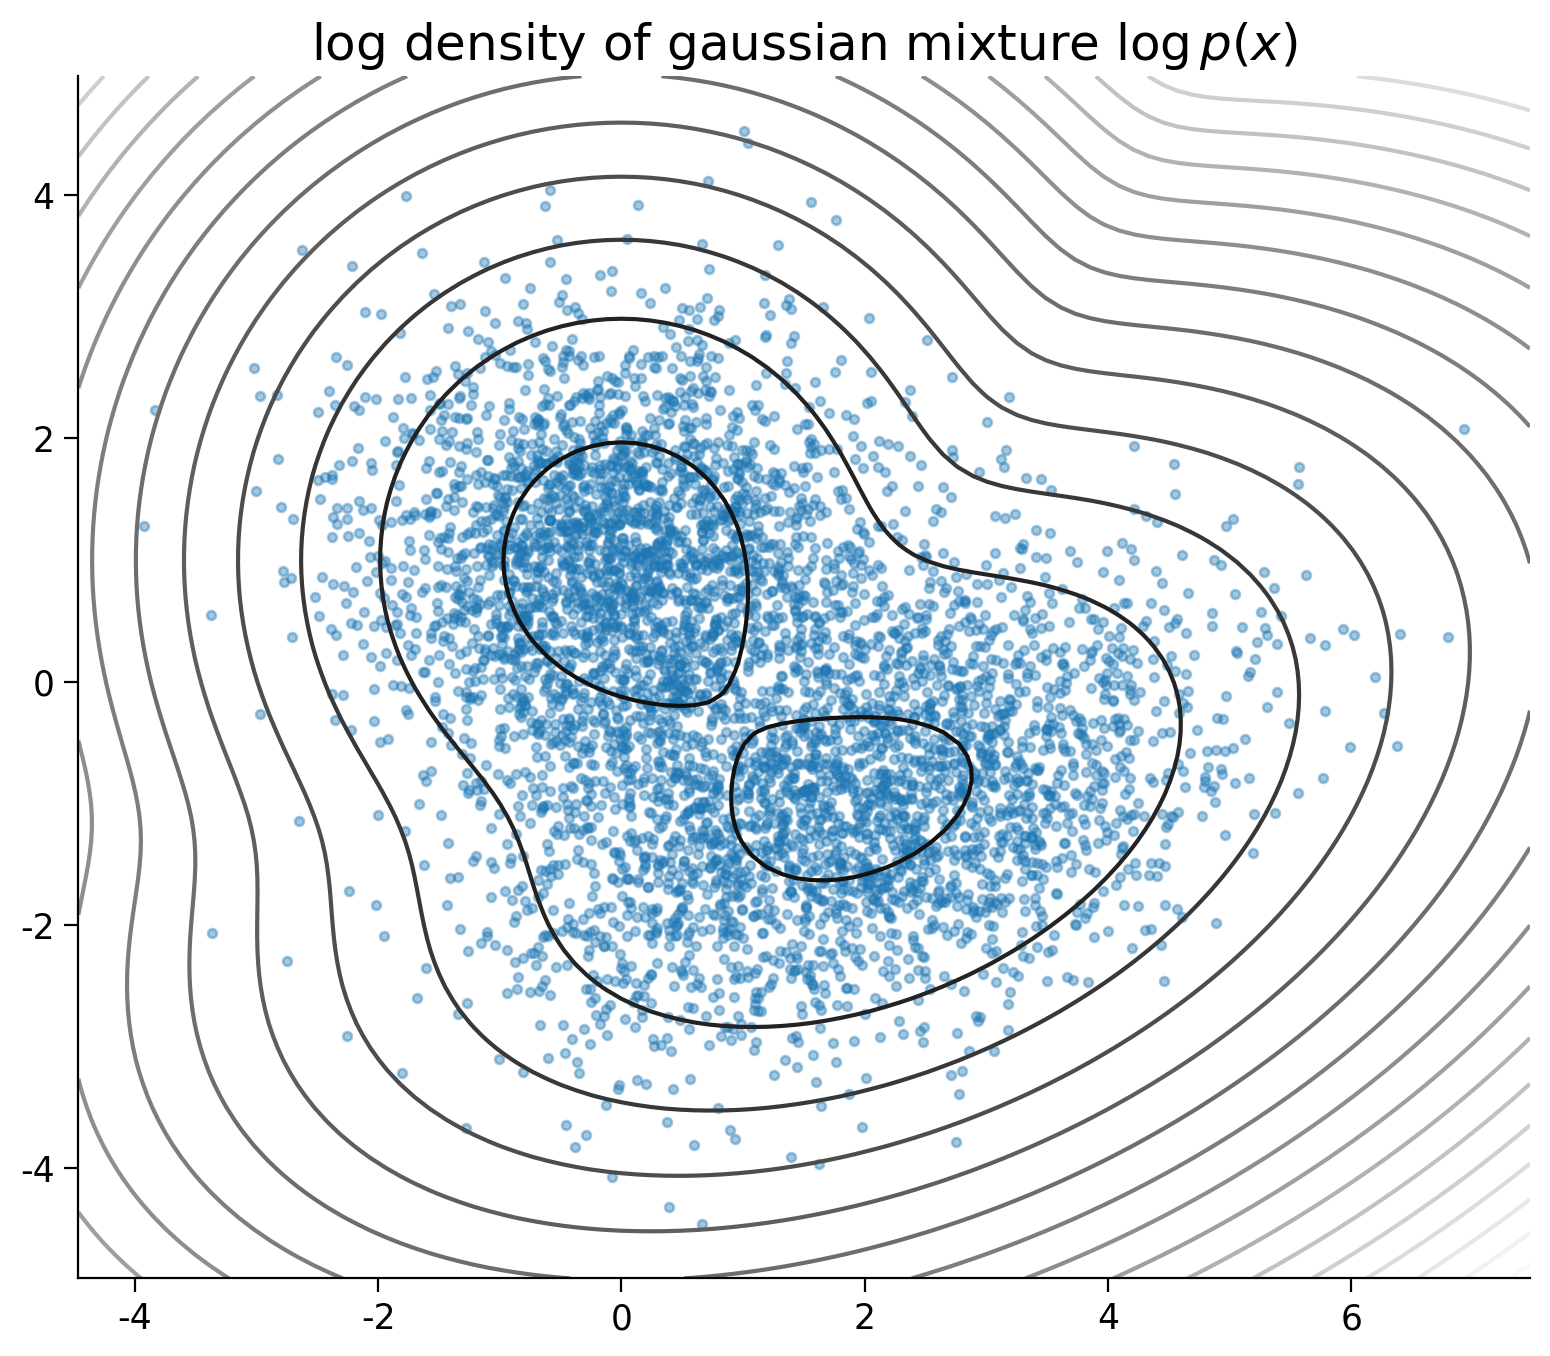
\includegraphics[width=\textwidth]{figures/D7.png}
            \caption{Stable Diffusion}
            \label{fig:stable_diffusion_example}
        \end{subfigure}
        \hfill
        \begin{subfigure}[b]{0.48\textwidth}
            \centering
            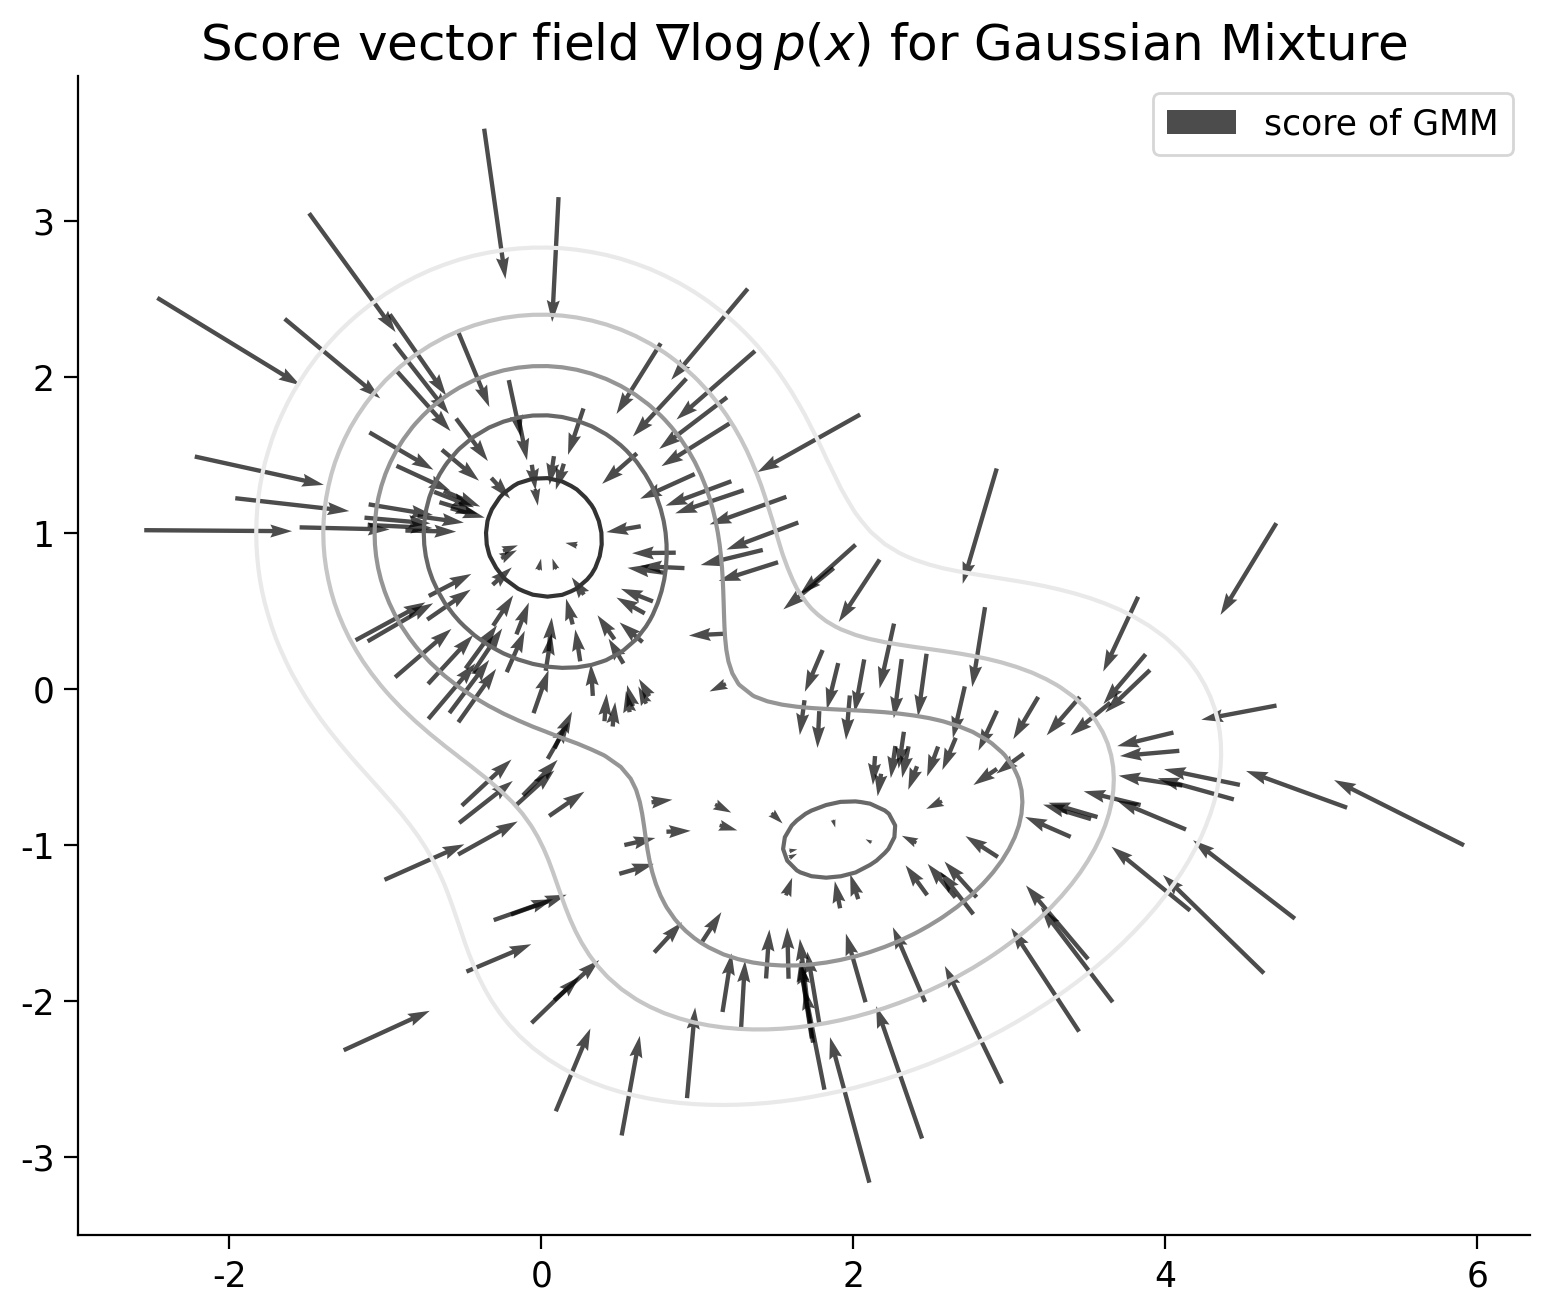
\includegraphics[width=\textwidth]{figures/D8.png}
            \caption{SDXL Turbo}
            \label{fig:sdxl_turbo_example}
        \end{subfigure}
        
        \vspace{1cm}

        \begin{subfigure}[b]{0.6\textwidth}
            \centering
            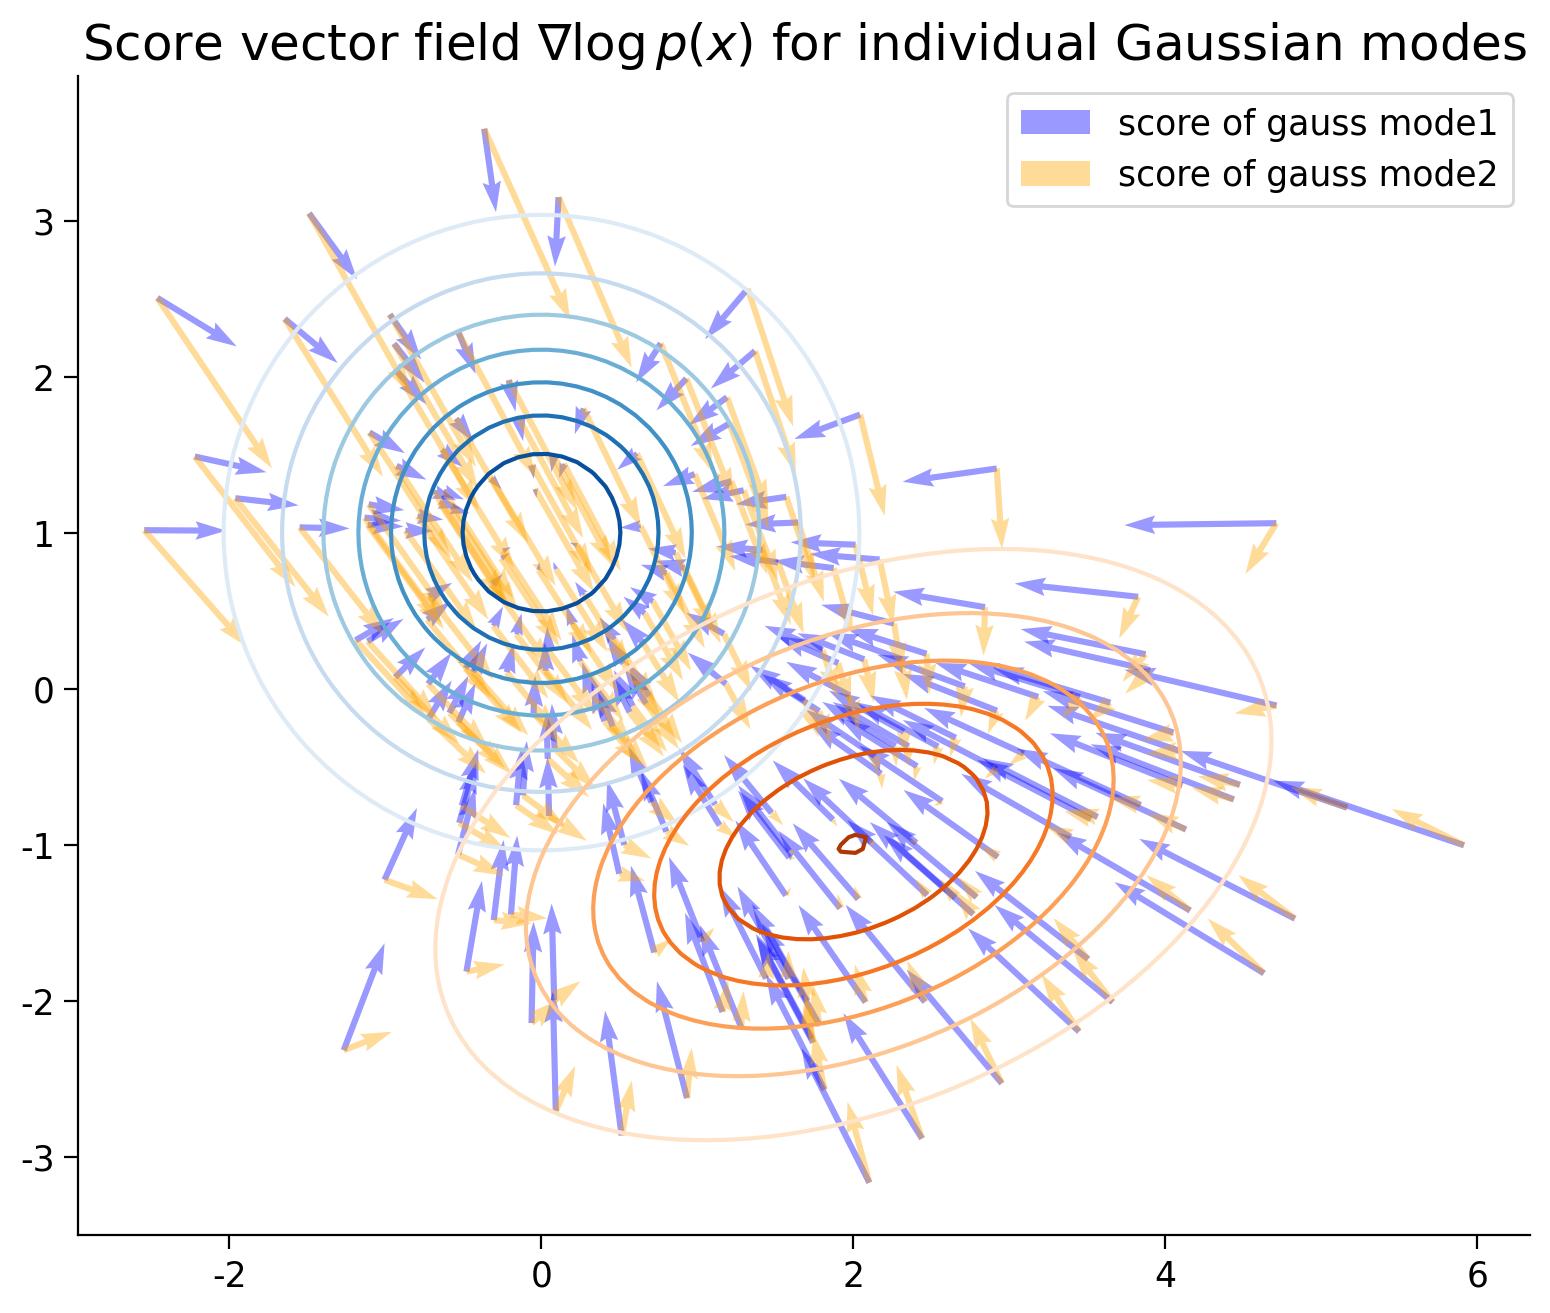
\includegraphics[width=\textwidth]{figures/D9.png}
            \caption{Stable Diffusion 3}
            \label{fig:sd3_example}
        \end{subfigure}
        \caption{不同文本到图像扩散模型生成的图像示例}
        \label{fig:diffusion_model_examples}
    \end{figure}

\end{itemize}

\section{大型语言模型(LLMs)的兴起}
\label{sec:llms}
大型语言模型(Large Language Models, LLMs),如OpenAI的GPT-3和GPT-4,是现代AI发展的集大成者。
\begin{itemize}
    \item \textbf{核心能力:} LLMs通过在海量的文本和代码数据上进行训练,学习到了强大的语言理解、生成和推理能力。它们不仅能生成流畅、连贯的文本,还能进行翻译、摘要、问答、代码生成,甚至进行一定程度的常识推理和逻辑推理。一个关键的发现是“涌现能力”(Emergent Abilities),即当模型的规模(参数量、数据量和计算量)超过某个阈值后,会突然展现出在小模型上不存在的新能力。
    \item \textbf{应用领域:} LLMs的应用已经渗透到各个领域,包括:
        \begin{itemize}
            \item \textbf{对话系统:} 如ChatGPT,能够进行开放域、多轮次的流畅对话。
            \item \textbf{内容创作:} 辅助撰写邮件、报告、营销文案和新闻稿等。
            \item \textbf{代码生成:} 如GitHub Copilot,能够根据自然语言描述自动生成代码片段。
            \item \textbf{知识问答与搜索:} 提供比传统搜索引擎更直接、更具概括性的答案。
        \end{itemize}
    \item \textbf{局限性与挑战:} 尽管能力强大,LLMs也面临着诸多挑战,包括:事实性错误(“幻觉”现象)、可能存在的偏见和歧视、高昂的训练和推理成本、以及其决策过程缺乏可解释性等。
\end{itemize}

\subsubsection*{案例研究:大型语言模型的规模效应与趋势}
\label{sssec:llm_case_study}
大型语言模型(LLMs)的革命性进展,在很大程度上归功于对其“规模效应”(Scaling Effect)的深刻理解和利用。研究发现,LLMs的性能与其规模——主要包括模型参数量(N)、训练数据集大小(D)和所用计算量(C)——之间存在着可预测的幂律关系(Power Law),这被称为\textbf{缩放法则(Scaling Laws)}。

\paragraph{1. 缩放法则的数学表达}
一个简化的缩放法则公式可以表示模型在给定计算预算下的最优损失(Loss)$L$与模型参数量$N$和训练数据量$D$的关系:
$$ L(N, D) = E + \frac{A}{N^\alpha} + \frac{B}{D^\beta} $$
其中,$E, A, B, \alpha, \beta$ 均为通过实验拟合得到的常数。该公式揭示了,为了达到最低的损失,模型的参数量和数据量需要协同增长。例如,DeepMind的Chinchilla模型研究发现,在给定计算量下,若要训练出最优模型,模型大小和训练数据量应大致保持1:1的比例增长。这一发现指导了后续LLMs(如Llama系列)更高效的训练策略。

\paragraph{2. 发展趋势的可视化分析}
近年来,对AI模型训练的投入呈现指数级增长。图 \ref{fig:llm_compute_trends} 展示了AI领域,特别是前沿LLMs,在训练计算量(以FLOPs为单位)上的惊人增长趋势。无论是通用模型还是特定领域的模型,其计算投入都大致遵循着每年数倍增长的规律。
\begin{figure}[H]
    \centering
    \begin{subfigure}[b]{0.48\textwidth}
        \centering
        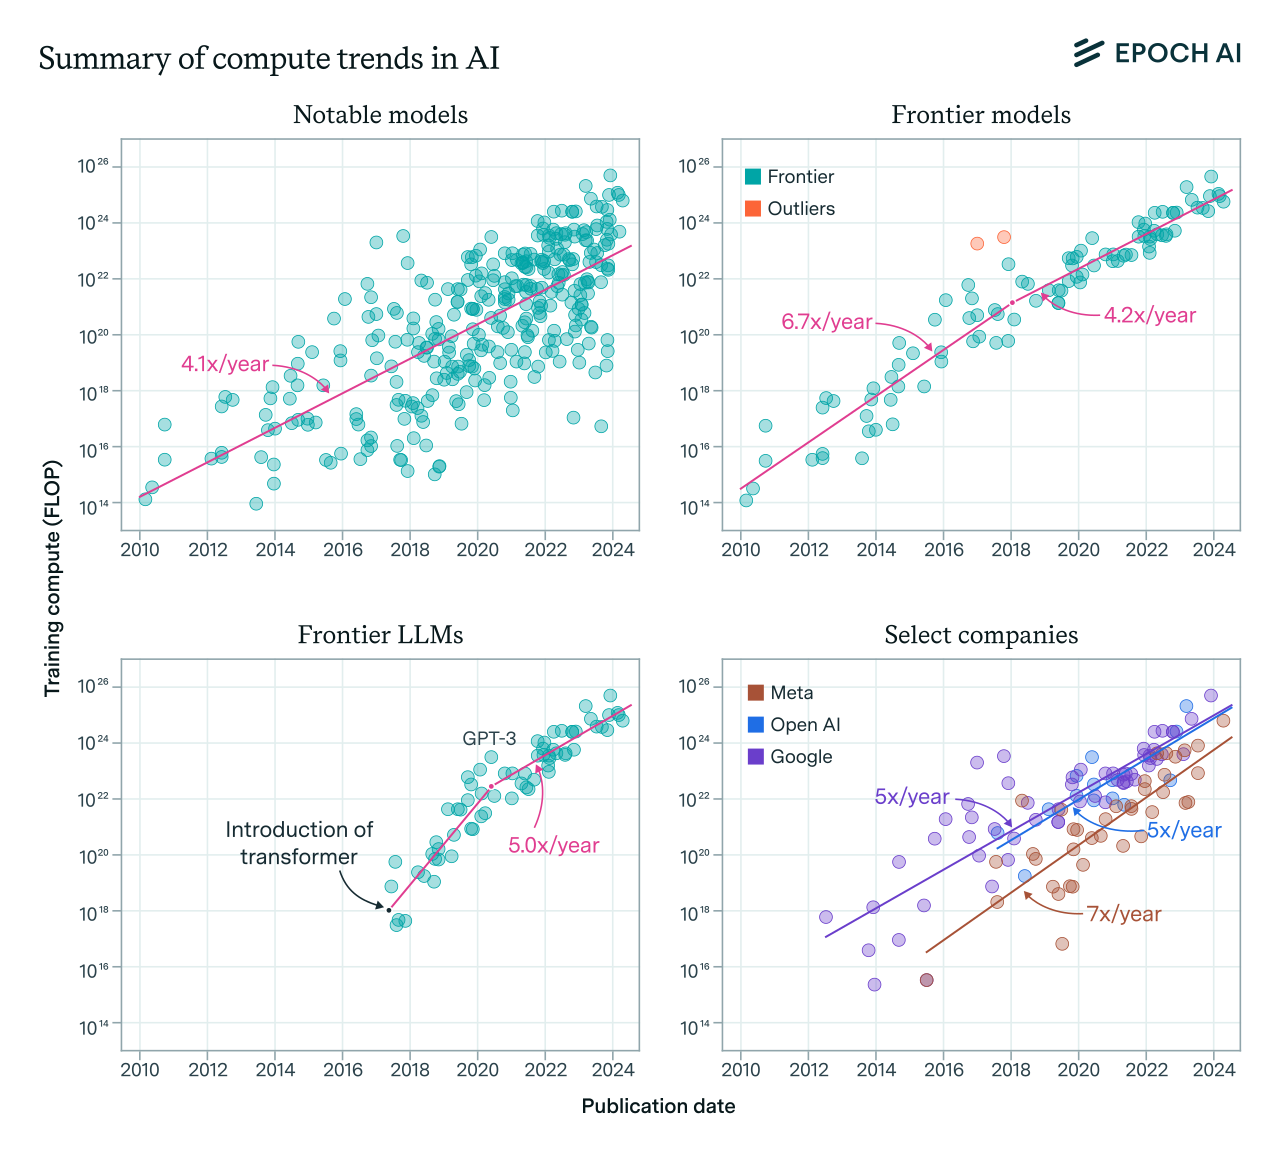
\includegraphics[width=\textwidth]{figures/LLM1.png}
        \caption{AI领域训练计算量的总体趋势}
        \label{fig:llm_compute_summary}
    \end{subfigure}
    \hfill
    \begin{subfigure}[b]{0.48\textwidth}
        \centering
        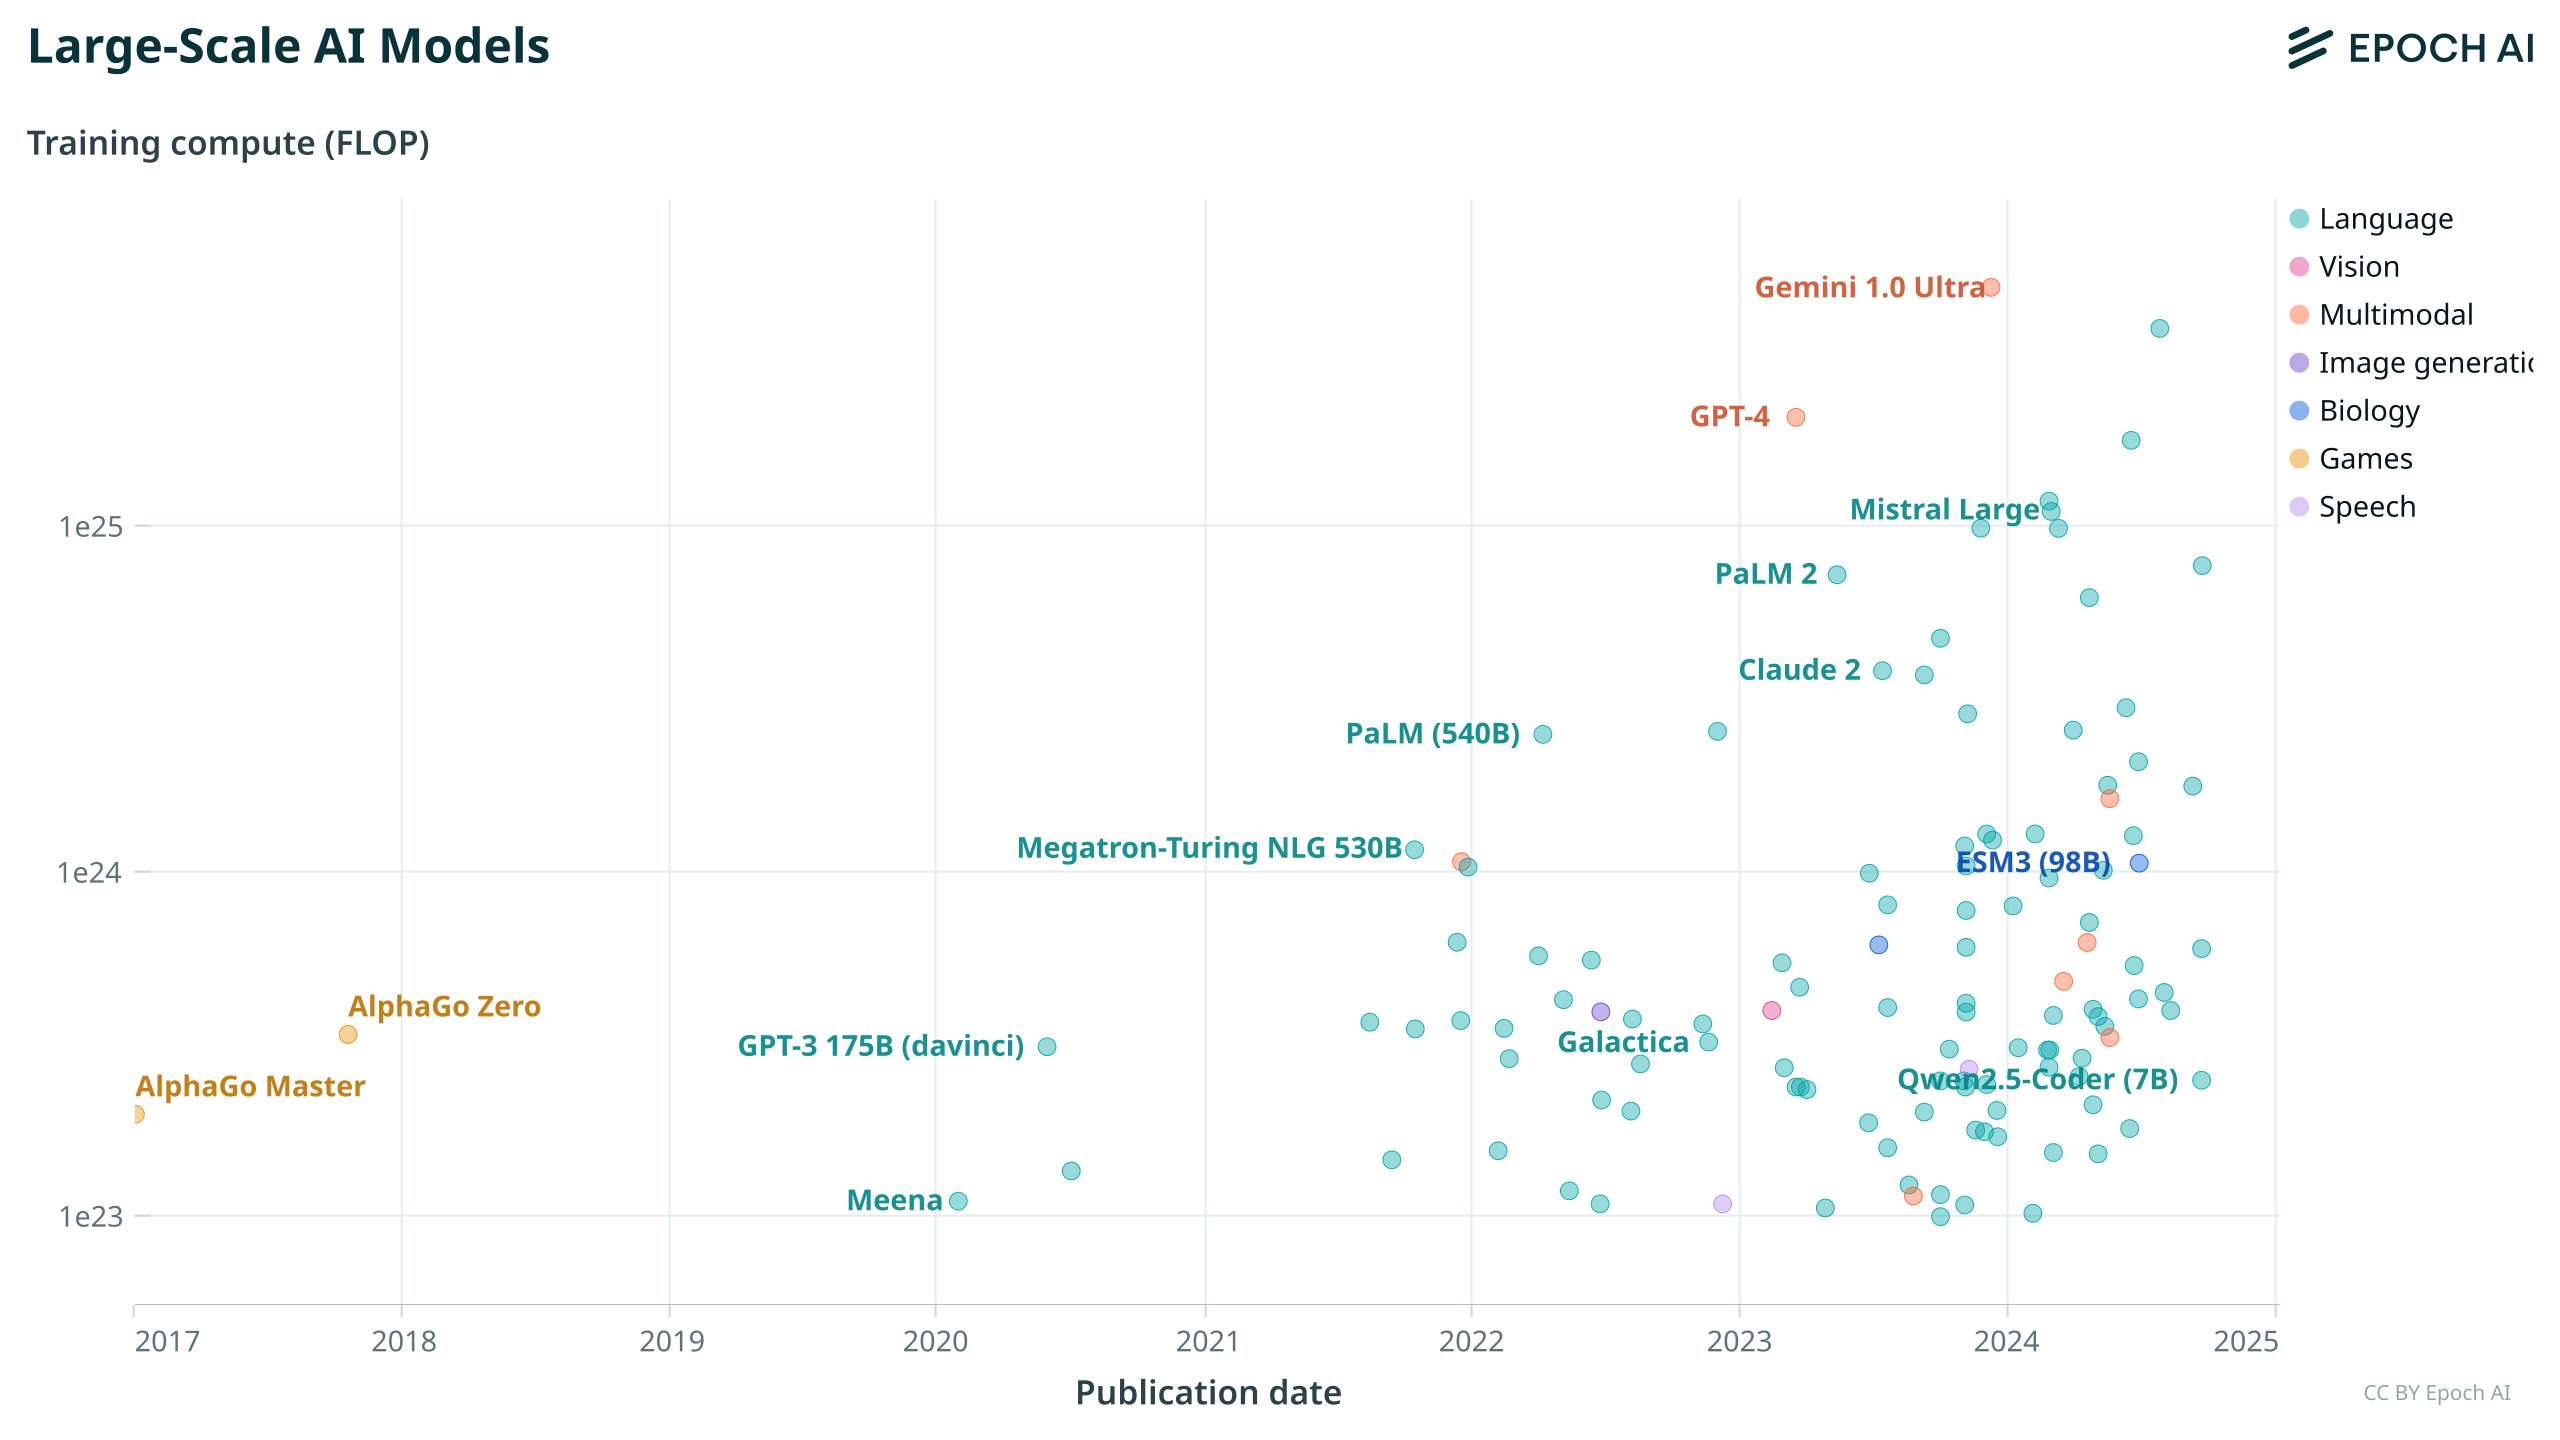
\includegraphics[width=\textwidth]{figures/LLM2.png}
        \caption{不同类型大型AI模型的计算量增长}
        \label{fig:llm_compute_by_type}
    \end{subfigure}
    \caption{AI模型训练计算量的指数级增长趋势}
    \label{fig:llm_compute_trends}
\end{figure}

这种指数级的计算投入直接转化为高昂的训练成本。如图 \ref{fig:llm_cost_perception}a 所示,从早期的Transformer模型到最新的Gemini Ultra,训练成本已从数千美元飙升至接近两亿美元。同时,模型的性能和行为也变得愈发复杂,使得如何评估和理解它们成为新的研究课题。图 \ref{fig:llm_cost_perception}b 则展示了人类对不同AI(包括早期的ELIZA和现代的LLMs)的识别原因分布,反映出随着模型能力的增强,其行为的“人性化”程度也在提高,对“图灵测试”提出了新的挑战。
\begin{figure}[H]
    \centering
    \begin{subfigure}[b]{0.48\textwidth}
        \centering
        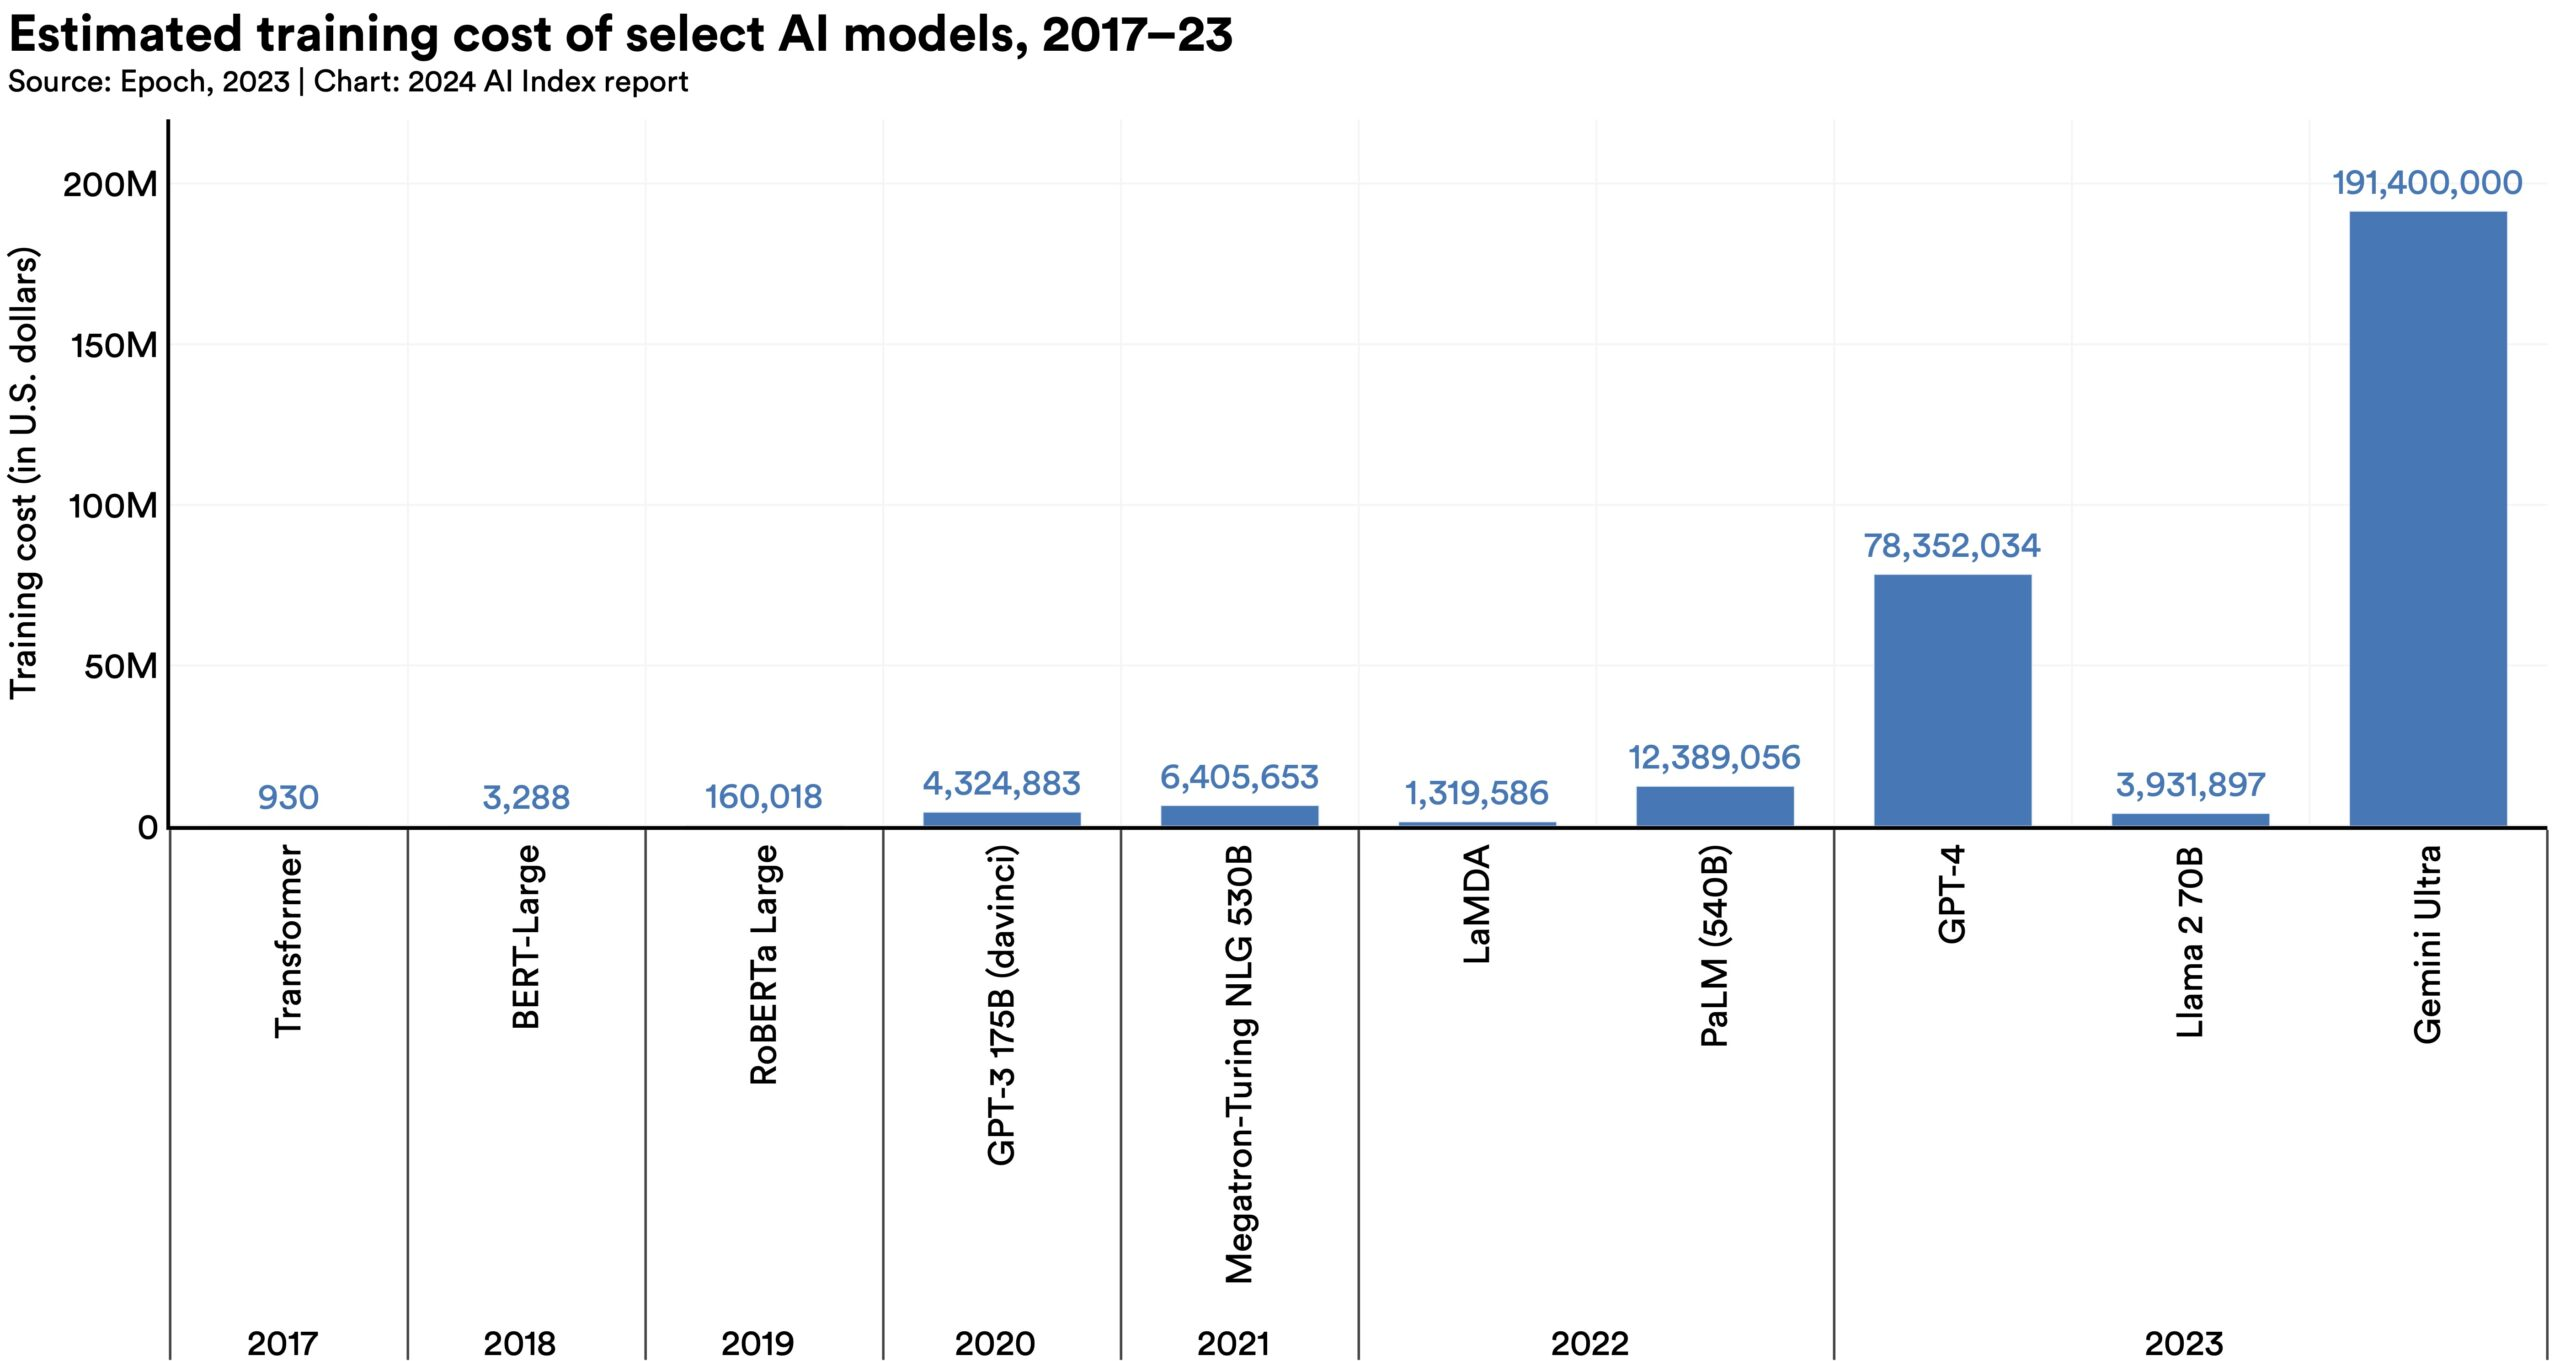
\includegraphics[width=\textwidth]{figures/LLM5.png}
        \caption{部分知名AI模型的预估训练成本}
        \label{fig:llm_training_cost}
    \end{subfigure}
    \hfill
    \begin{subfigure}[b]{0.48\textwidth}
        \centering
        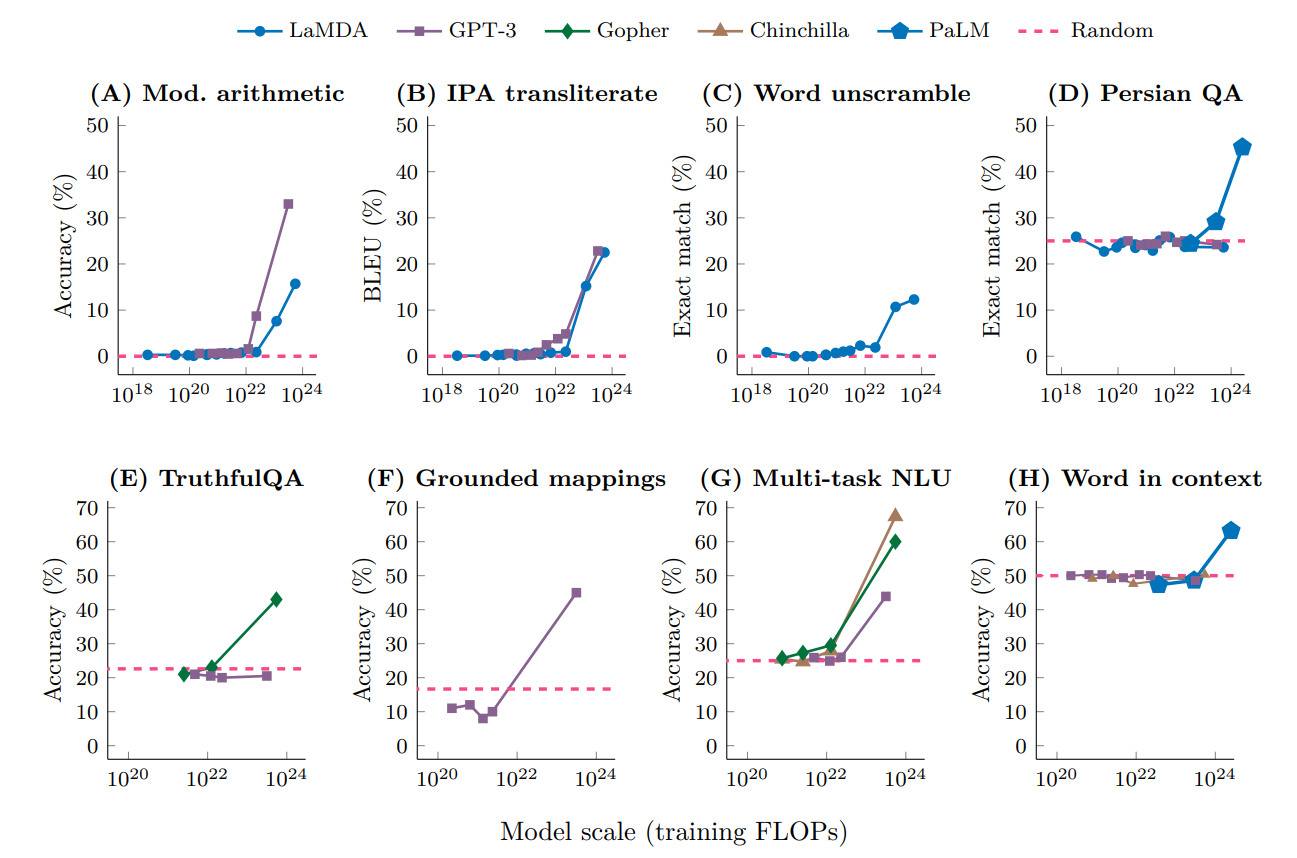
\includegraphics[width=\textwidth]{figures/LLM6.png}
        \caption{人类判断不同AI为“人工智能”的原因分布}
        \label{fig:llm_reason_class}
    \end{subfigure}
    \caption{大型AI模型的训练成本与人类感知分析}
    \label{fig:llm_cost_perception}
\end{figure}

\paragraph{3. 模型性能与置信度校准}
随着模型规模的扩大,其输出的准确性与自身的置信度(Confidence)之间的关系变得至关重要。一个“校准良好”的模型,其预测的置信度应该能真实反映其预测的正确率。图 \ref{fig:llm_confidence_calibration} 展示了不同LLMs在与人类的对比测试中的准确率与置信度的关系。理想情况下,准确率应随置信度的增加而提高。这些图表揭示了不同模型在“自我认知”能力上的差异,这是评估其可靠性和可信度的重要维度。
\begin{figure}[H]
    \centering
    \begin{subfigure}[b]{0.48\textwidth}
        \centering
        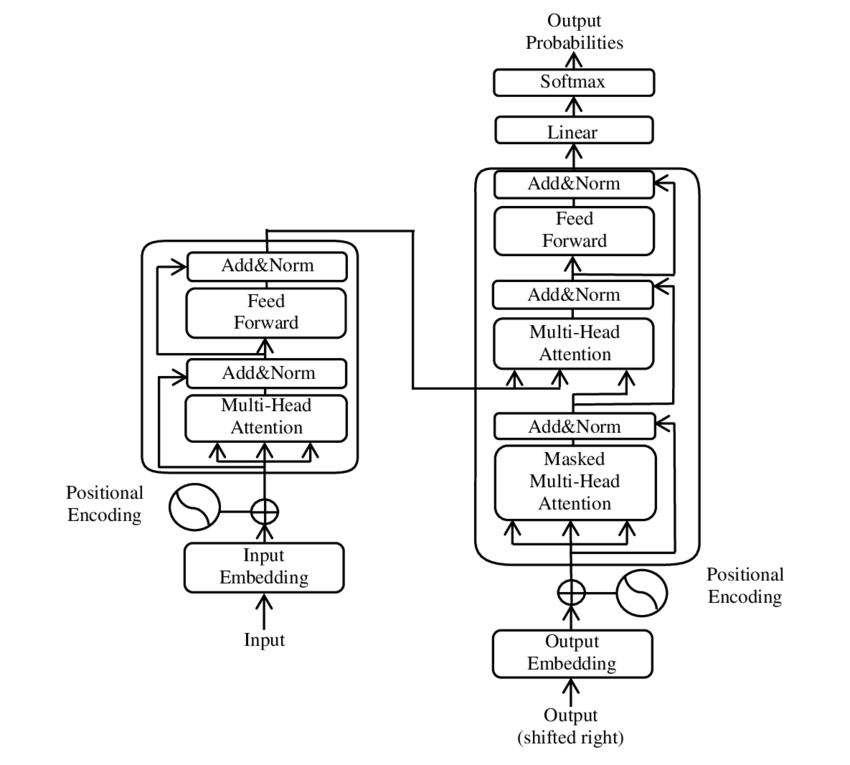
\includegraphics[width=\textwidth]{figures/LLM3.png}
        \caption{不同AI的准确率与置信度关系}
        \label{fig:llm_accuracy_confidence}
    \end{subfigure}
    \hfill
    \begin{subfigure}[b]{0.48\textwidth}
        \centering
        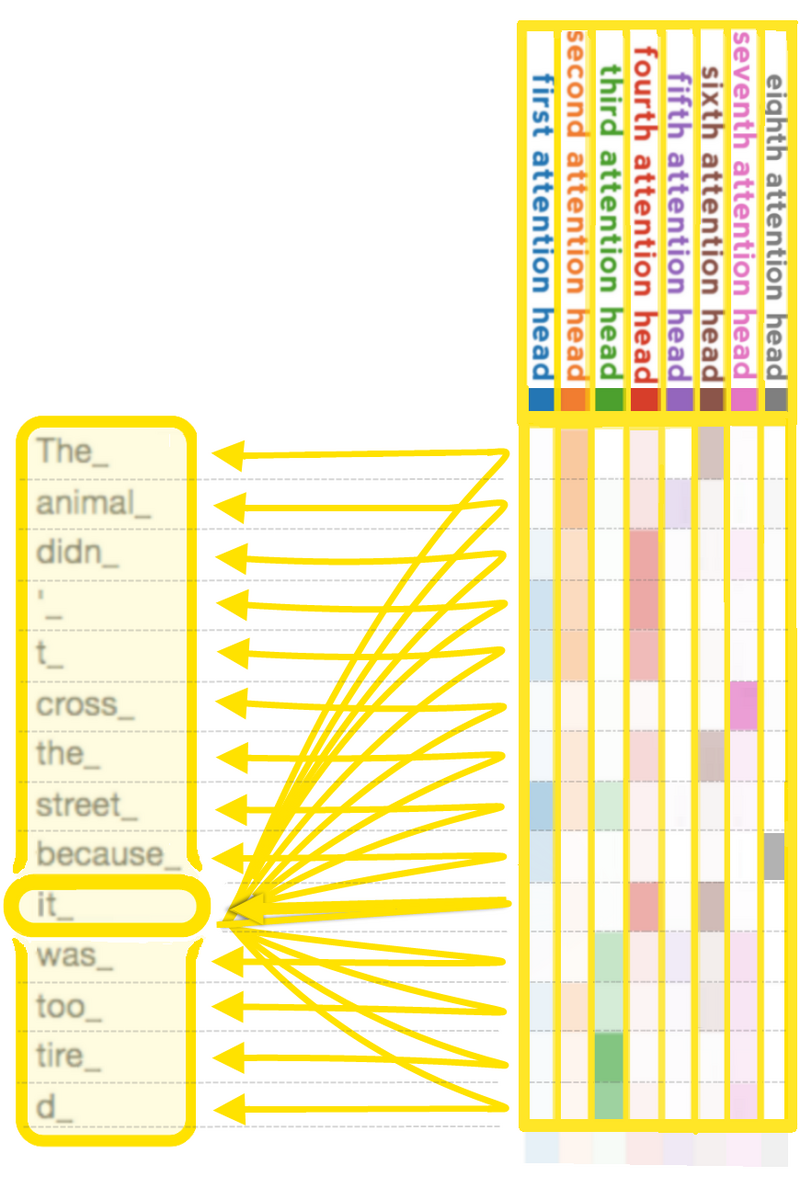
\includegraphics[width=\textwidth]{figures/LLM4.png}
        \caption{不同AI在对比测试中的胜率与置信度}
        \label{fig:llm_winrate_confidence}
    \end{subfigure}
    \caption{大型语言模型的置信度校准与性能评估}
    \label{fig:llm_confidence_calibration}
\end{figure}

\section{其他新兴技术}
\label{sec:emerging_tech}
除了上述主流技术外,一些新兴的技术方向也在不断拓展着人工智能的边界。
\begin{itemize}
    \item \textbf{联邦学习(Federated Learning):} 联邦学习是一种分布式的机器学习范式,它允许在多个持有本地数据的设备(如手机)上协同训练一个模型,而无需将原始数据集中上传到服务器。这在保护用户数据隐私和安全方面具有巨大优势,特别适用于金融、医疗等对数据安全要求极高的领域。
    \item \textbf{边缘AI(Edge AI):} 边缘AI指的是将AI 模型的训练和推理过程直接在数据产生的源头——即边缘设备(如智能摄像头、工业传感器和可穿戴设备)上执行。这可以显著降低延迟、减少对网络带宽的依赖,并增强数据的实时处理能力和隐私保护。
    \item \textbf{多模态AI(Multimodal AI):} 多模态AI旨在让模型能够同时理解和处理来自不同模态的信息,如文本、图像、语音和视频。通过融合多模态信息,模型可以获得对世界更全面、更深入的理解,从而在诸如视频内容理解、图文生成和情感计算等任务中表现出更强的能力。
\end{itemize}

\section{总结}
\label{sec:conclusion_chap2}
本章详细阐述了驱动现代人工智能发展的各项关键技术。从监督学习、无监督学习到强化学习这三大经典机器学习范式,为AI提供了基础的理论框架。深度学习的崛起,特别是CNN 在视觉领域的突破、RNN/LSTM对序列数据的处理能力,以及Transformer架构对自然语言处理的颠覆,共同构成了现代AI技术的核心支柱。在此基础上,生成式AI(如GANs 和扩散模型)赋予了机器前所未有的创造力,而大型语言模型的兴起则将AI的通用能力推向了新的高度。最后,联邦学习、边缘AI和多模态 AI等新兴技术,正从隐私保护、部署效率和信息融合等多个维度,进一步拓展着人工智能的未来版图。这些技术相互交织、共同演进,正在深刻地重塑着科技和社会的面貌。